\documentclass[oribibl]{llncs}

\usepackage{booktabs} % For formal tables

%%%%%%%%%%%%%%%%%%%%%%%%%%%%%%%%%%%%%%%%%%%%%%%%%%%%%%%%%%%%%%%%%%%%%%%%%%%%%%%%%
%%%%%%%%%%%%%%%%%%%%%%%%%%%%%%% customize begin %%%%%%%%%%%%%%%%%%%%%%%%%%%%%%%%
% \usepackage{appendix}
\usepackage{amsfonts}
\usepackage{enumerate,paralist}
\usepackage{mathtools}
\usepackage{amsmath}
\usepackage{stmaryrd}

\usepackage{tikz,pgffor}
\usetikzlibrary{arrows}
\usetikzlibrary{shapes}
\usetikzlibrary{calc}
\usetikzlibrary{automata}
\usetikzlibrary{positioning}

\tikzstyle{location} = [
    rectangle,
    rounded corners,
    draw=black,
    very thick,
    minimum height=2em,
    inner sep=0pt,
    text centered
]
\tikzstyle{tran}  = [
    draw,
    ->,
    >=stealth,
    rounded corners
]
\tikzstyle{nchoice}  = [
    draw,
    >=stealth,
    rounded corners
]
\tikzstyle{pchoice}  = [
    draw,
    ->,
    >=stealth,
    rounded corners,
    dashed
]
\tikzstyle{dec}   = [inner sep=0pt]
\tikzstyle{mode}  = [
    shape=circle,
    draw,
    inner sep=0pt,
    minimum size=5mm
]

%\theoremstyle{plain}
%\newtheorem{lemma}{Lemma}
%\newtheorem{claim}{Claim}
%\newtheorem{proposition}{Proposition}
%\newtheorem{definition}{Definition}
%\newtheorem{corollary}{Corollary}
%\newtheorem{theorem}{Theorem}
%\newtheorem{example}{Example}
%\newtheorem{remark}{Remark}
%\newtheorem{observation}{Observation}
%\newtheorem{assumption}{Assumption}

%% Notations

%%General Notations

\newcommand{\Rset}{\mathbb{R}}
\newcommand{\Nset}{\mathbb{N}}
\newcommand{\Zset}{\mathbb{Z}}
\newcommand{\ap}{\mbox{\sl AP}}
\newcommand{\opt}{\mbox{\sl opt}}

%%Clocks and Clock Constraints

\newcommand{\clocks}{\mathcal{X}}
\newcommand{\val}[1]{\mbox{\sl Val}\left(#1\right)}
\newcommand{\reset}[2]{{#1}{\left[#2:=0\right]}}
\newcommand{\add}[2]{{#1}{+}{#2}}
\newcommand{\zero}{\mathbf{0}}
\newcommand{\true}{\mathbf{true}}
\newcommand{\false}{\mathbf{false}}
\newcommand{\supp}[1]{{\mbox{\sl supp}}(#1)}
\newcommand{\dist}[1]{{\mathcal{D}}{\left(#1\right)}}
\newcommand{\sat}[1]{{\llbracket}{#1}{\rrbracket}}
\newcommand{\intp}[1]{{\lfloor}{#1}{\rfloor}}
\newcommand{\fracp}[1]{\mbox{\sl frac}(#1)}
\newcommand{\evclass}[1]{\left[#1\right]}

%%PTAs

\newcommand{\pta}{\mathcal{C}}
\newcommand{\locs}{L}
\newcommand{\loc}{\ell}
\newcommand{\acts}{\mbox{\sl Act}}
\newcommand{\inv}{\mbox{\sl inv}}
\newcommand{\enab}{\mbox{\sl enab}}
\newcommand{\penab}[2]{\mbox{\sl enab}\left(
    {#1},{#2}
\right ) }
\newcommand{\prob}{\mbox{\sl prob}}
\newcommand{\lbfunc}{\mathcal{L}}
\newcommand{\clcons}[1]{\mbox{\sl CC}\left(#1\right)}
\newcommand{\istate}{\left(\loc^*,\mathbf{0}\right)}

%% Semantics of PTAs

\newcommand{\states}{S}
\newcommand{\trans}{\rightarrow}
\newcommand{\tran}[3]{{#1}{\xrightarrow{#2}}{#3}}
\newcommand{\probk}{\mathbf{P}}

\newcommand{\fnpaths }[1]{\mbox{\sl Paths}^*_{#1}}
\newcommand{\infpaths}[1]{\mbox{\sl Paths}^\omega_{#1}}
\newcommand{\omgpaths}[2]{\mbox{\sl Reach}^{#2}_{#1}}
\newcommand{\initloc }[1]{\mbox{\sl init}\left(#1\right)}
\newcommand{\lastloc }[1]{\mbox{\sl last}\left(#1\right)}

\newcommand{\fnpath}{\rho}
\newcommand{\infpath}{\pi}

\newcommand{\length}[1]{\left| #1 \right|}

%% Notations for Probability Space

\newcommand{\probm}{\mathbb{P}}
\newcommand{\expv}{\mathbb{E}}
\newcommand{\cyl}{\mbox{\sl Cyl}}

%% Notations for DTAs

\newcommand{\dta}{\mathcal{A}}
\newcommand{\dtloc}{q}
\newcommand{\dtclocks}{\mathcal{Y}}
\newcommand{\cstates}{Q}
\newcommand{\alphabet}{\Sigma}
\newcommand{\rules}{\Delta}
\newcommand{\dtphi}[3]{\Phi_{#1,#2}^{#3}}
\newcommand{\dtx}[3]{\mathbf{X}_{#1,#2}^{#3}}
\newcommand{\dtq}[3]{\mathbf{q}_{#1,#2}^{#3}}
\newcommand{\trfunc}{\kappa}
\newcommand{\dtatr}[3]{{#1}{\xRightarrow{#2}}{#3}}
\newcommand{\regions}{\mathcal{G}}

\newcommand{\run}[3]{{#1}_{#2}\left(#3\right)}
\newcommand{\iconfig}{\left(\dtloc^*,\mathbf{0}\right)}

%%Product Constrution
\newcommand{\product}[2]{{#1}{\otimes}{#2}}
\newcommand{\pr}[2]{\mathfrak{p}_{#1}^{#2}}
\newcommand{\pfunc}{\mathcal{T}}
\newcommand{\sfunc}{\theta}
\newcommand{\acc}[2]{{\mbox{\sl AccPaths}}_{#1}^{#2}}
\newcommand{\extactions}{\mathcal{B}}
\newcommand{\exttuples}{\mathcal{T}}

%%Reward Structure
\newcommand{\rcum}{\mathbf{r}_{\locs}}
\newcommand{\rinst}{\mathbf{r}_{\acts}}
\newcommand{\ronestep}{\mathbf{r}}
\newcommand{\accum}[1]{\mbox{\sl Cum}_{#1}}
\newcommand{\rd}[2]{\mathsf{R}_{#1}^{#2}}

%%Rabin acceptance

% \newcommand{\infset}[1]{\mbox{\sl{inf  }} ( #1 )}
% \newcommand{\trace }[1]{\mbox{\sl{trace}} ( #1 )}
% \newcommand{\traj  }[1]{\mbox{\sl{traj }} ( #1 )}
\newcommand{\infset}[1]{\mbox{\sl inf}  ( #1 )}
\newcommand{\trace }[1]{\mbox{\sl trace}( #1 )}
\newcommand{\traj  }[1]{\mbox{\sl traj} ( #1 )}
\newcommand{\rabin}{\mathcal{F}}

%%Finite acceptance
\newcommand{\fstates}{F}

\newcommand{\Lang}[2] {
    \mbox{\sl AccPaths}
        _{#1}
        ^{#2}
}

\newcommand{\rabinp}[1]{\mbox{\sl RPaths}_{#1}}

\newcommand{\Accept}[1]{
    \mbox{\sl RabinPaths}
        _{#1}
        % ^{#2}
}

\newcommand{\LangCsAqF}{
    \Lang
        {\pta,\sigma}
        {\dta,\dtloc}
}

\newcommand{\AcceptCxAqsF}{
    \Accept
        {
            \product{\pta}{\dta_\dtloc},
            \sigma
        }
        % {\rabin}
}

\newcommand{\TLang}{
    \pfunc\left(
        \LangCsAqF
    \right)
}

\newcommand{\TAcc}{
%    \Accept
%        {
%            \product{\pta}{\dta_\dtloc},
%            \sfunc \left(
%                \sigma
%            \right)
%        }
    \rabinp{\sfunc\left(\sigma\right)}
        % {\rabin}
}
\newcommand{\accept}[2]{
    \mbox{\bf ACC} \left(
      {#1},
      {#2}
    \right)
}
\newcommand{\acccept}[3]{
    \mbox{\bf ACC} \left(
      {#1},
      {#2},
      {#3}
    \right)
}
\newcommand{\accccept}[4]{
    \mbox{\bf ACC} \left(
      {#1},
      {#2},
      {#3},
      {#4}
    \right)
}
%% Proudct
\newcommand{\Region}[1]{
  \mbox{Reg}[
    {#1}
  ]
}
\newcommand{\WAIT}[0]{\mbox{\sl WAIT}}
\newcommand{\WORK}[1]{\mbox{\sl WORK}_{#1}}
\newcommand{\DONE}[1]{\mbox{\sl DONE}_{#1}}
\newcommand{\request}[1]{\mbox{\sl Req}_{#1}}
\newcommand{\p}[1]{\mbox{\sl p}_{#1}}

\def\INIT{  \mbox{\sl INIT} }
\def\FAIL{  \mbox{\sl FAIL} }
\newcommand{\q}[1]{\mbox{\sl q}_{#1}}

\newcommand{\location}[5]{
    \node[location] (#1) at #2 {
        \begin{tabular}{c}
            \ensuremath{#3} \\
            \hline
            \ensuremath{#4} \\
            \ensuremath{#5}
        \end{tabular}
    }
}

\newcommand{\PairV}[2]{#1#2}
\newcommand{\PairS}[2]{({#1},{#2})}

%%For drawing grids

\newcounter{row}
\newcounter{col}

\newcommand\setrow[3]{
  \setcounter{col}{1}
  \foreach \n in {#1, #2, #3} {
    \edef\x{\value{col} - 0.5}
    \edef\y{3.5 - \value{row}}
    \node[anchor=center] at (\x, \y) {\n};
    \stepcounter{col}
  }
  \stepcounter{row}
}

% Undecidability
\newcommand{\nta}{\mathcal{A}}
\newcommand{\qinit}{q_{\mbox{\sl\scriptsize init} }}
\newcommand{\qstart}{q_{\mbox{\sl\scriptsize start}}}
\newcommand{\ntaap}[1]{b_{#1}}
\newcommand{\PCswLang}{
    \probm^{\pta,\sigma_w }\left(
    \Lang
        {\pta,\sigma_w}
        {\nta',\qinit,\rabin}
    \right)
}

\newcommand{\TRA}{TRA}
\newcommand{\tra}{\mathcal{A}}

% INF MDP
\newcommand{\clocksX}{\mathcal{X}}
\newcommand{\clocksY}{\mathcal{Y}}
\newcommand{\reg}{R}
\newcommand{\floor}[1]{\mbox{\sl floor} \left (
    {#1}
\right )}
\newcommand{\productmdp}[2]{{#1}{\ast}{#2}}
\newcommand{\mdploc}{s}
\newcommand{\project}[2]{
    {#1} \downarrow {#2}
}
\newcommand{\pair}[2]{
    \left (
        {#1}
        ,
        {#2}
    \right )
}
\newcommand{\clocksALL}{
    \clocksX \cup \left(
        \bigcup_{k=1}^{n} \clocksY_k
    \right )
}
%%%%%%%%%%%%%%%%%%%%%%%%%%%%%% customize end %%%%%%%%%%%%%%%%%%%%%%%%%%%%%%
%%%%%%%%%%%%%%%%%%%%%%%%%%%%%%%%%%%%%%%%%%%%%%%%%%%%%%%%%%%%%%%%%%%%%%%%%%%

% Copyright
% \setcopyright{none}
%\setcopyright{acmcopyright}
%\setcopyright{acmlicensed}
%%%%%% \setcopyright{rightsretained}
%\setcopyright{usgov}
%\setcopyright{usgovmixed}
%\setcopyright{cagov}
%\setcopyright{cagovmixed}


% DOI
% \acmDOI{10.475/123_4}

% ISBN
% \acmISBN{123-4567-24-567/08/06}

%Conference
%\acmConference[HSCC 2018]{ACM International Conference on Hybrid Systems: Computation and Control }{April 2018}{
%  Porto, Portugal
%}
% \acmConference{HSCC 2018}{April 2018}{
%   Porto, Portugal
% }
% \acmYear{1997}
% \copyrightyear{2017}

% \acmPrice{15.00}


\begin{document}
\title{Verifying Probabilistic Timed Automata Against \\Omega-Regular Dense-Time Properties}
% \subtitle{Verifying PTAs Against Timed-Automata Specifications}
% \titlenote{Produces the permission block, and
%   copyright information}
% \subtitlenote{The full version of the author's guide is available as
%   \texttt{acmart.pdf} document}

\author{
    Hongfei Fu\inst{1} 
    \and 
    Yi Li\inst{2} 
    \and 
    Jianlin Li\inst{3,4}
    % \and
    % Lijun Zhang\inst{4}
}
\institute{
    Shanghai Jiao Tong University, Shanghai, China
    % ,\\ \email{fuhf@cs.sjtu.edu.cn}
    \and
    Department of Informatics, School of Mathematical Sciences, Peking University, Beijing, China 
    % \\ \email{liyi\_math@pku.edu.cn}
    \and
    State Key Laboratory of Computer Science, Institute of Software, Chinese Academy of Sciences, Beijing, China
    \and
    College of Computer Science and Technology, Nanjing University of Aeronautics and Astronautics, Nanjing, China
    % \email{ljlin@nuaa.edu.cn}
    % State Key Laboratory of Computer Science, Institute of Software, Chinese Academy of Sciences, Beijing, China \\
    % \email{zhanglj@ios.ac.cn}
}

% \author{Hongfei Fu}
% % \authornote{Dr.~Trovato insisted his name be first.}
% % \orcid{1234-5678-9012}
% \affiliation{%
%   \institution{Shanghai Jiao Tong University}
%   % \streetaddress{P.O. Box 1212}
%   % \city{Shanghai}
%   % \state{China}
%   % \postcode{43017-6221}
% }
% \email{fuhf@ios.ac.cn}

% \author{Yi Li}
% % \authornote{The secretary disavows any knowledge of this author's actions.}
% \affiliation{%
%   \institution{Department of Informatics, School of Mathematical Sciences, Peking University}
%   % \streetaddress{P.O. Box 1212}
%   % \city{Beijing}
%   % \state{China}
%   % \postcode{43017-6221}
% }
% \email{liyi_math@pku.edu.cn}

% \author{Jianlin Li}
% \affiliation{%
%   \institution{College of Computer Science and Technology Nanjing University of Aeronautics and Astronautics}
%   % \streetaddress{P.O. Box 1212}
%   % \city{Beijing}
%   % \state{China}
%   % \postcode{43017-6221}
% }
% \email{ljlin@nuaa.edu.cn}

% \author{Lijun Zhang}
% \affiliation{%
%   \institution{State Key Laboratory of Computer Science, Institute of Software, Chinese Academy of Sciences}
%   % \streetaddress{P.O. Box 1212}
%   % \city{Beijing}
%   % \state{China}
%   % \postcode{43017-6221}
% }
% \email{zhanglj@ios.ac.cn}

% \author{Aparna Patel}
% \affiliation{%
%  \institution{Rajiv Gandhi University}
%  \streetaddress{Rono-Hills}
%  \city{Doimukh}
%  \state{Arunachal Pradesh}
%  \country{India}}
% \author{Huifen Chan}
% \affiliation{%
%   \institution{Tsinghua University}
%   \streetaddress{30 Shuangqing Rd}
%   \city{Haidian Qu}
%   \state{Beijing Shi}
%   \country{China}
% }

% The default list of authors is too long for headers}
% \renewcommand{\shortauthors}{B. Trovato et al.}

% \begin{comment}
% % \begin{abstract}
% % This paper provides a sample of a \LaTeX\ document which conforms,
% % somewhat loosely, to the formatting guidelines for
% % ACM SIG Proceedings.\footnote{This is an abstract footnote}
% % \end{abstract}

% %
% % The code below should be generated by the tool at
% % http://dl.acm.org/ccs.cfm
% % Please copy and paste the code instead of the example below.
% %
% \begin{CCSXML}
% <ccs2012>
%  <concept>
%   <concept_id>10010520.10010553.10010562</concept_id>
%   <concept_desc>Computer systems organization~Embedded systems</concept_desc>
%   <concept_significance>500</concept_significance>
%  </concept>
%  <concept>
%   <concept_id>10010520.10010575.10010755</concept_id>
%   <concept_desc>Computer systems organization~Redundancy</concept_desc>
%   <concept_significance>300</concept_significance>
%  </concept>
%  <concept>
%   <concept_id>10010520.10010553.10010554</concept_id>
%   <concept_desc>Computer systems organization~Robotics</concept_desc>
%   <concept_significance>100</concept_significance>
%  </concept>
%  <concept>
%   <concept_id>10003033.10003083.10003095</concept_id>
%   <concept_desc>Networks~Network reliability</concept_desc>
%   <concept_significance>100</concept_significance>
%  </concept>
% </ccs2012>
% \end{CCSXML}

% \ccsdesc[500]{Computer systems organization~Embedded systems}
% \ccsdesc[300]{Computer systems organization~Redundancy}
% \ccsdesc{Computer systems organization~Robotics}
% \ccsdesc[100]{Networks~Network reliability}


% \keywords{ACM proceedings, \LaTeX, text tagging}
% \end{comment}

\maketitle

\vspace{-2em}

\begin{abstract}
\label{sec:abstract}

%% 1. what is the problem 
Scientific applications that run on leadership computing facilities often face the challenge 
of being unable to fit leading science cases onto accelerator devices due to memory constraints 
(memory-bound applications).
%
% 2. what is your solution 
In this work, the authors studied one such US Department of Energy mission-critical condensed matter 
physics application, Dynamical Cluster Approximation (DCA++), and this paper discusses how device memory-bound challenges were successfully reduced  by proposing an effective 
``all-to-all'' communication method---a ring communication algorithm. 
%
This implementation takes advantage of acceleration on GPUs and remote direct memory access (RDMA) for fast data exchange between GPUs. 
%
\\Additionally, the ring algorithm was optimized with sub-ring communicators
and multi-threaded support to further reduce communication overhead and 
expose more concurrency, respectively.
%
% 3. What's the cherry-picked evaluation result you want to mention
The computation and communication were also analyzed 
by using the Autonomic Performance Environment for Exascale 
(APEX) profiling tool,  and this paper further discusses the 
performance trade-off for the ring algorithm implementation. 
%
The memory analysis on the ring algorithm shows that the allocation size for the authors' most 
memory-intensive data structure per GPU is now reduced to $1/p$ of the original size, where $p$ is the number of GPUs in the ring communicator.
%
The communication analysis suggests that 
the distributed Quantum Monte Carlo execution time grows linearly as sub-ring size increases, and the cost of messages passing through the network interface connector could be a limiting factor.


%
% \todoRed{Ronnie: Next sentence needs rewrite, too much information about Green's function that no one knows in the abstract; recommend generalizing.} \emph {However, DCA++ is currently facing memory-bound challenge as 
% a larger device array $G_t$ is limited by device memory size, where
% $G_t$ is a two-particle Green's function that allows condensed matter
% scientists to explore larger and more complex (higher fidelity)
% physics cases.}

\end{abstract}

\keywords{DCA++, Quantum Monte Carlo, GPU Remote Direct Memory Access, memory-bound issue, exascale machines}


\vspace{-1em}

\section{Introduction}  \label{sec:introduction}

\newcommand\inexpIntro[3]{#1?(#2,#3).}
\newcommand\rinexpIntro[3]{*#1?(#2,#3).}
\newcommand\outexpIntro[3]{#1!(#2,#3).}
\newcommand\outatomIntro[3]{#1!(#2,#3)}

We propose a fully automated method for proving termination of \(\pi\)-calculus processes.
Although there have been a lot of studies on termination analysis for the \(\pi\)-calculus
and related calculi~\cite{Deng06IC,Demangeon07,SangiorgiTermination,KobayashiHybrid,Yoshida04IC,DBLP:journals/jlp/DemangeonHS10,Venet98SAS}, most of them have been rather theoretical,
and there have been surprisingly little efforts in developing  fully automated termination
verification methods and tools based on them. To our knowledge,
Kobayashi's \typical{}~\cite{TyPiCal,KobayashiHybrid} is the only exception that
can prove termination of \(\pi\)-calculus processes (extended with natural numbers)
fully automatically, but its termination analysis is quite limited (see Section~\ref{sec:relatedwork}).

Our method is based on a reduction to termination analysis for sequential programs:
we translate a \(\pi\)-calculus process \(P\) to a sequential program \(S_P\), so that
if \(S_P\) is terminating, so is \(P\). The reduction allows us to use
powerful, mature methods and tools
for termination analysis of sequential programs~\cite{heizmann2016ultimate,freqterm,DBLP:conf/lics/PodelskiR04,Kuwahara2014Termination,DBLP:journals/cacm/CookPR11}.

The idea of the translation is to convert a chain of communications on replicated input
channels to a chain of recursive function calls of the target sequential program.
Let us consider the following Fibonacci process:
\begin{align*}
    & \rinexpIntro{\fib}{n}{r}
        \ifexp{n<2}{ \soutatom{r}{1} \\ &\quad}
                   { \nuexp{s_1} \nuexp{s_2} (\outatomIntro{\fib}{n-1}{s_1} \PAR \outatomIntro{\fib}{n-2}{s_2} \PAR \sinexp{s_1}{x}\sinexp{s_2}{y}\soutatom{r}{x+y}) \\}
    & \PAR \outatomIntro{\fib}{m}{r}
\end{align*}
Here, the process
$\rinexpIntro{\fib}{n}{r} \ldots$ is a function server that computes the \(n\)-th Fibonacci number
in parallel and returns the result to \(r\),
and $\outatom{\fib}{m}{r}$ sends a request for computing the \(m\)-th Fibonacci number;
those who are not familiar with the syntax of the \(\pi\)-calculus may wish to consult
Section~\ref{sec:targetlanguage} first.
To prove that the process above is terminating for any integer \(m\),
it suffices to show that there is no infinite chain of communications on $\fib$:
\[
    \fib(m,r) \to \fib(m_1,r_1) \to \fib(m_2,r_2) \to \cdots.
\]
We convert the process above to the following program:\footnote{The actual translation
  given later is a little more complex.}
\begin{verbatim}
 let rec fib(n) = if n<2 then () else (fib(n-1) [] fib(n-2)) in
 fib(m)
\end{verbatim}
Here, \texttt{[]} represents the non-deterministic choice.
Note that, although the calculation of Fibonacci numbers is not preserved,
for each chain of communications on \texttt{fib}, there is a corresponding
sequence of recursive calls:
\[
\mathtt{fib}(m) \to \mathtt{fib}(m_1) \to \mathtt{fib}(m_2) \to \cdots.
\]
Thus, the termination of the sequential program above implies the termination of
the original process.
As shown in the example above, (i) each communication on a replicated input channel
is converted to a function call, (ii) each communication on a non-replicated input
channel is just removed (or, in the actual translation, replaced by a call of
a trivial function defined by \(f(\seq{x})=(\,)\)), and (iii) parallel composition
is replaced by a non-deterministic choice.
We formalize the translation outlined above and prove its correctness.

The basic translation sketched above sometimes loses too much information.
For example, consider the following process:
\begin{align*}
    & \rinexpIntro{\pre}{n}{r} \soutatom{r}{n-1} \\
    & \PAR \rinexpIntro{f}{n}{r} \ifexp{n<0}{ \soutatom{r}{1} }
                                       { \nuexp{s} (\outatomIntro{\pre}{n}{s} \PAR \sinexp{s}{x}\outatomIntro{f}{x}{r}) } \\
    & \PAR \outatomIntro{f}{m}{r}
\end{align*}
The translation sketched above would yield:
\begin{verbatim}
  let pred(n) = n-1 in
  let rec f(n) = if n<0 then () else (pred(n) [] f(*)) in
  f(m)
\end{verbatim}
Here, \texttt{*} represents a non-deterministic integer: since we have removed
the input $\sinatom{s}{x}$, we do not have information about the value of \( x \).
As a result, the sequential program above is non-terminating, although the original
process is terminating.
To remedy this problem, we also refine the basic translation above by using a refinement
type system for the \(\pi\)-calculus. Using the refinement type system,
we can infer that the value of \(x\) in the original process is less than \(n\),
so that we can refine the definition of \texttt{f} to:
\begin{verbatim}
 let rec f(n) = ... else (pred(n) [] let x=* in assume(x<n);f(x))
\end{verbatim}
The target program is now terminating, from which
we can deduce that the original process is also terminating.
We have implemented an automated tool based on the refined translation above.

The contributions of this paper are summarized as follows.
\begin{itemize}
\item The formalization of the basic translation from the \(\pi\)-calculus
  (extended with integers) to sequential programs, and a proof of its correctness.
\item The formalization of a refined translation based on a refinement type system.
\item An implementation of the refined translation, including automated refinement type
  inference based on CHC solving, and experiments to evaluate the effectiveness of
  our method.
\end{itemize}

The rest of this paper is structured as follows.
Section~\ref{sec:targetlanguage} introduces the source and target languages
of our translation.
Section~\ref{sec:approach} 
formalizes the basic translation, and proves its correctness.
Section~\ref{sec:refinement} refines the basic translation by using a refinement type system.
Section~\ref{sec:implementation} reports an implementation and experiments.
Section~\ref{sec:relatedwork} discusses related work,
and Section~\ref{sec:conclusion} concludes the paper.

\section{Preliminaries}\label{chpt:preliminiaries}
In this chapter we will introduce some of the mathematical background and notation needed for this thesis. In particular, we will shortly introduce the differential geometric description of spacetime in Section \ref{sec:spacetime_geometry} and give an introduction to the notion of global hyperbolicity and its connection to Green- and normally-hyperbolic operators in Section \ref{sec:global_hyperbolicity}. In a bit more detail, we will introduce the notion of differential forms and give explicit definitions, also in terms of an index based notation, in Section \ref{sec:differential_forms}. For completeness, in Section \ref{sec:cat-theory}, we present basic definitions of category theory. The reader familiar with these topics can safely skip this chapter and refer to it when interested in the chosen conventions.
%
%
%
%
%%%%%%
%%SPACTIME GEOMETRY
%%%%%
%
%
%
\subsection{Spacetime geometry}\label{sec:spacetime_geometry}
In GR, the universe is mathematically described as a four dimensional \emph{spacetime}, consisting of a smooth, four dimensional manifold \gls{M} (assumed to be Hausdorff, connected, oriented, time-oriented and para-compact) and a Lorentzian metric $g$. We will assume the signature of the Lorentzian metric $g$ to be $(-,+,+,+)$. The Levi-Civita connection on $(\M,g)$ is as usual denoted by \gls{nabla}.
Throughout this thesis, we treat spacetime as fixed, implementing a gravitational background determined classically by Einstein's field equations. Hence, we neglect any back-reaction of the fields on the metric, both in the quantum and the classical case. In that sense, we treat the fields as \emph{test fields}.\par
For the basic mathematical theory regarding Lorentzian manifolds, we refer to the literature: An introduction to the topic with an emphasis on the physical application in GR is for example given in \cite{wald_GR} and \cite{carroll_spacetime-and-gr}.
Here, we will shortly recap the notion of a tangent space and tangent bundle and generalize to the notion of a vector bundle which we will use in the general description of normally hyperbolic operators and differential forms.
In the following, we generalize the setting to an arbitrary smooth manifold $\N$ of dimension $N$ with either Lorentzian or Riemannian metric $k$.\par
%
%
A \emph{tangent vector} $v_x$ at point $x \in \N$ is a linear map $v_x : C^\infty(\N , \IR) \to \IR$ that obeys the Leibniz rule, that is, for $f,g \in C^\infty (\N,\IR)$ it holds $v_x(fg) = f(x)v_x(g) + v_x(f)g(x)$.
We define the \emph{tangent space} \gls{TxN} of $\N$ at $x$ as the real $N$-dimensional vector space of all tangent vectors at point $x$.
The disjoint union of all tangent spaces is called the \emph{tangent bundle} \gls{TN} of $\N$ and is itself a manifold of dimension $2N$. A \emph{vector field} is a map $v: \N \to T\N$ such that $v(x) \in T_x\N$.
The respective dual spaces, that is the space of all linear functionals, the \emph{co-tangent space} and the \emph{co-tangent bundle}, are denoted by \gls{TsxN} and \gls{TsN} respectively.\par
%
For Lorentzian manifolds, we call a tangent vector $v$ at $x \in \N$ \emph{timelike} if $k_{\mu \nu} v^\mu v^\nu < 0$, \emph{spacelike} if $k_{\mu \nu} v^\mu v^\nu > 0$ and \emph{null} (or lightlike) if $k_{\mu \nu} v^\mu v^\nu = 0$. At every point $x \in \N$, we define the set of all \emph{causal}, that is, either timelike or null, tangent vectors in the tangent space at $x$. This set is called the \emph{light cone} at $x$ and it is split up into two distinct parts, one that we call the future light cone, and one that we call the past light cone at $x$. Since we assume the manifold to be time orientable, there exists a smooth vector field $t$ that is timelike at every $x \in \N$. Given this time orientation, we identify the future (past) light cone with the set of tangent vectors $v \in T_x\N$ such that $k_{\mu\nu} v^\mu t^\nu < 0$ (respectively $> 0$). Therefore, a tangent vector $v$ at $x$ is called \emph{future directed} (past directed) if it lies in the future (past) light cone at $x$.\\
Accordingly, a curve $\gamma : I \to \N$ is called timelike (spacelike, null, causal, future or past directed) if its tangent vector $\dot{\gamma}$ is timelike (spacelike, null, causal, future or past directed) at every $x \in \N$.  For every point $x \in \N$ we define the \emph{causal future/past} \gls{causalfuturepast} of $x$ as the set of all points $q \in \N$ that can be reached by a future directed causal curve originating in $x$. For any subset $S \in \N$ we define $J^\pm (S) = \bigcup_{x \in S} J^\pm(x)$ and $J(S) = J^+(S) \cup J^- (S)$. Finally, the future/past domain of dependence $\gls{futurepastdomainofdependence}$ of a set $S \subset \N$ is the set of all points $x \in \N$ such that every inextendible causal curve through $x$ intersects $S$. The \emph{domain of dependence} \gls{domainofdependence} of $S$ is the union of the future and past domain of dependence of the set $S$.
For more details on the causal structure of spacetime we refer to for example \cite[Chapter 8]{wald_GR}.\par
%
%
%
The notion of tangent bundles can be generalized to the notion of a vector bundle. Instead of ``attaching'' the vector spaces $T_x \N$ to every point $x$ of the manifold, we allow for the occurrence of arbitrary vector spaces, called the fibres of the vector bundle. A vector bundle then consists of the base manifold, in our case $\N$, the total space and a map $\pi$ from the total space to the base manifold, that can be locally trivialized. At each point of the base manifold, the pre-image of $\pi$ is the fibre of the vector bundle. To be precise we define, following \cite{rudolph_schmidt}:
\begin{definition}[Vector bundle]
	A smooth \emph{vector bundle} over $\N$ is a tuple $\gls{vectorbundle} = (E,\N, \pi)$, where $E$ is a smooth manifold and $\pi : E \to \N$ is a smooth surjective map satisfying:
	\begin{enumerate}
		\item For every $x \in \N$, $\pi^{-1}(x)$ is a vector space, called the fibre of the bundle at point $x$.
		\item There exists a finite dimensional vector space $F$, an open covering $\left\{ U_\alpha\right\}_\alpha$ of $\N$ and a family of diffeomorphisms $\chi_\alpha : \pi^{-1}(U_\alpha) \to U_\alpha \times F$ such that for all $\alpha$ it holds $\chi_\alpha \comp \text{pr}_1 =  \restr{\pi}{\pi^{-1}(U_\alpha)}$ and for every $x \in \N$ the map $\text{pr}_2 \comp \restr{\chi_\alpha}{\pi^{-1}(x)} : \pi^{-1}(x) \to F$ is linear.
	\end{enumerate}
\end{definition}
Here, the maps $\text{pr}_1$ and $\text{pr}_2$ denote the projection onto the first respectively second component of an element in $U_\alpha \times F$. The properties graphically mean that \emph{locally}, the vector bundle ``looks like" the product of the base manifold with the fibre. The tuples $(U_\alpha, \chi_\alpha)$ are called \emph{local trivializations} of the vector bundle. Like for vector spaces, we can define the sum and product of vector bundles, by using the according vector space definitions on the fibres of the bundle.\par
Let $\mathfrak{X}, \mathfrak{Y}$ be vector bundles over $\N$ with fibres $X_x$ and $Y_x$ at $x \in \N$. We denote by \gls{whitneysum} the \emph{Whitney sum} of the two vector bundles - the vector bundle over $\N$ whose fibres are given by the direct sum $X_x \oplus Y_x$. Similarly, one obtains the local trivializations of the Whitney sum from the trivializations of $\mathfrak{X}, \mathfrak{Y}$ and direct sums.\par
Accordingly, let $\mathfrak{X}, \mathfrak{Y}$ be vector bundles over $\N$ and $\widetilde{\N}$, with fibres $X_x$ and $Y_{\tilde{x}}$ at $x \in \N$, $\tilde{x} \in \widetilde{\N}$ respectively. We denote by \gls{outerproductbundle} the \emph{outer product} of the two vector bundles - the vector bundle over $\N \times \widetilde{\N}$ whose fibres are given by the tensor products $X_x \otimes Y_x$. Similarly, one obtains the local trivializations of the outer product from the trivializations of $\mathfrak{X}, \mathfrak{Y}$ and tensor products. \par
%
Finally, we generalize the notion of vector fields:
\begin{definition}[Sections of vector bundles]
Let $\mathfrak{X}=(E,\N,\pi)$ be a vector bundle with fibres $X_x=\pi^{-1}(x)$ at $x \in \N$. A \emph{smooth section} of the vector bundle is a smooth map $\gamma : \N \to E$ such that $\gamma(x) \in X_x$ for all $x \in \N$. The \emph{vector space of smooth sections} of $\mathfrak{X}$ is denoted by \gls{gammax}, the one with compactly supported sections is as usual denoted by \gls{gammaxzero}.
\end{definition}
In this language, a vector field $v$ is just a smooth section of the tangent bundle of a manifold, $v \in \Gamma(T\N)$. One may therefore identify the physical notion of fields with smooth sections of vector bundles. This point of view will be used to define the notion of differential forms in Section \ref{sec:differential_forms}.\par
In this thesis, we usually are interested in complex valued functions (or sections in general). Therefore, we view all occurring vector bundles as complex, in the sense that we take two distinct copies of the vector bundle, one representing the real, one the imaginary part of the bundle. A section of that complex vector bundle is just a pair of two sections of the real vector bundle under consideration. From now, if not specified explicitly, we will view all vector bundles, including the tangent bundle $T\N$, as complex vector bundles. Accordingly, smooth sections of those bundles will in general be complex valued.
%
%
%
%
%
%
%
%
%%%%%%%
%%PARTIAL DIFFERENTIAL OPERATORS AND GLOBAL HYPERBOLICITY
%%%%%%%
%
%
%
\subsection{Partial differential operators and global hyperbolicity}\label{sec:global_hyperbolicity}
When dealing with field theories, whether classical or quantum, one is, of course, interested in the dynamics of the fields. These are usually described by some partial differential equation, often of second order. In the following, we give a short introduction to the theory of certain partial differential operators acting on smooth sections of a vector bundle over the spacetime $(\M,g)$.\par
%
As we have seen, these smooth sections are generalizations of the notion of a field.  In the following, let $\mathfrak{X}$ denote a vector bundle over the manifold $\M$ and let $P: \Gamma(\mathfrak{X}) \to \Gamma(\mathfrak{X})$ be a partial differential operator acting on smooth sections of the bundle. As in the case of flat spacetime, we are interested in basic questions regarding the differential equation $Pf = j$, for example: Can we formulate a (globally) well posed initial value problem? Does the differential equation possess (unique) solutions? To answer these questions, we will now restrict to the case where $P$ is linear and of second order, as it is often the case in physical applications. One can show that for a certain class of such operators, namely normally hyperbolic partial differential operators of second order, we can rigorously treat these questions.\par
Choosing local coordinates $x=(x_\mu)$ on $\M$ and a local trivialization of $\mathfrak{X}$, a linear partial differential operator of second order is called \emph{normally hyperbolic} if it takes the form
\begin{align}
	P = - \sum_{\mu,\nu} g^{\mu \nu} \partial_\mu \partial_\nu + \sum_{\alpha} A_\alpha (x) \partial_\alpha + B(x) \formspace,
\end{align}
where $A_\alpha$ and $B$ are matrix-valued coefficients depending smoothly on the coordinate $x$ (see. \cite[Chapter 1.5]{baer_ginoux_pfaeffle}). One can also formulate a coordinate independent definition in terms of the principal symbol, which we will not present here (see for example \cite[Section 1.5]{baer_ginoux_pfaeffle} ). \par
%
Normally hyperbolic operators possess unique fundamental solutions (see for example the fundamental solutions to the wave operator as noted in Lemma \ref{lem:fundamental_solution_wave_operator}). These fundamental solutions fulfill certain physically important properties, such as a finite propagation speed smaller than the speed of light. Furthermore, specifying the initial data on some space-like hypersurface $X \in  \M$ specifies a unique solution on the domain of dependence $D(X)$ of $X$. Due to these properties, one often calls normally hyperbolic operators just \emph{wave operators}. But to state a \emph{globally} well posed initial value problem for a wave equation, we need to restrict the class of spacetimes $\M$ under consideration to those that possess space-like hypersurfaces $X$ whose domain of dependence is all of the spacetime, $D(X) = \M$. This leads to the notion of \emph{globally hyperbolic} spacetimes:
\begin{definition}[Global Hyperbolicity]
	A spacetime $\M$ is called \emph{globally hyperbolic} if there exists a Cauchy surface $\gls{sigma}$ in $\M$.
\end{definition}
\noindent Here, a Cauchy surface is a space-like hypersurface $\Sigma \subset \M$ such that every inextendible causal curve $\gamma$ intersects $\Sigma$ exactly once. One can show that Cauchy surfaces fulfill the desired property mentioned above, that is,  $D(\Sigma) = \M$. Furthermore, one can show that any globally hyperbolic spacetime $\M$ is foliated by a one-parameter family $\left\{ \Sigma_t \right\}_t$ of Cauchy surfaces (see for example \cite[Theorem 8.3.14]{wald_GR}). \par
In physical applications, one often finds the dynamics of a theory to be described by wave operators. Most prominently, the Klein-Gordon operator $(\square + m^2)$ acting on scalar fields, or its generalization, the wave operator acting on differential forms introduced in Section \ref{sec:differential_forms}, is normally hyperbolic. But there are also important physical field theories that are not described by wave operators, such as the Proca field treated in this thesis. It turns out that the Proca operator (see Definition \ref{def:proca_operator}) is a so called \emph{Green-hyperbolic} operator. These are again partial differential operators $P$ of second order acting on smooth sections of some vector bundle, such that $P$ (and its dual $P'$) posses fundamental solutions. Obviously, normally hyperbolic operators are Green-hyperbolic, but the opposite is not true. One can generalize some results obtained by studying normally hyperbolic operators to Green-hyperbolic operators. An introduction to this topic is given in \cite{baer_green-hyperbolic}, where it is also shown that the Proca operator is Green-hyperbolic but not normally hyperbolic.\par
For our application, the notion of Green-hyperbolicity is not of vast importance, but it is worth mentioning that there exists a more detailed mathematical background on the treatment of such operators.
A very detailed description of normally hyperbolic operators on Lorentzian manifolds, including proofs of the above statements regarding the initial value problem and the existence of fundamental solutions, is given in \cite{baer_ginoux_pfaeffle}, also with an overview of quantization. A shorter introduction to the topic is for example treated in \cite{baer-ginoux_classical-and-quantum-fields}, also with a description of quantization.
%
%
%
%
%
%
%%%
%
%
%
%%
%%%%%%%%%
%%%DIFFERENTIAL FORMS
%%%%%%%%
%
%
%
\subsection{Differential forms}\label{sec:differential_forms}
%
%
Differential forms provide an elegant, coordinate independent description of calculus on smooth manifolds. In particular, they generalize the notion of line- and volume-integrals that are known from analysis. Differential forms play a remarkable role in physics, as one can argue that they indeed describe fundamental physical entities. As an example, instead of viewing a classical force as a vector, one can think of it, more closely related to experiments, as a differential one-form that assigns a scalar to a tangent vector of a curve. This scalar is the (infinitesimal) work associated with the force along the curve. Also, differential forms allow for an elegant geometric description of field theories, for example the Maxwell and Proca field theories that we encounter in this thesis. In Maxwell's classical theory of electromagnetism, instead of viewing the electric and magnetic field (which are conceptually just forces) as the fundamental physical entities, one introduces the \emph{vector potential}, a one-form, consisting of the scalar electric potential and the vector potential associated with the magnet field. Experiments like the Aharonov-Bohm experiment allow for an interpretation of the vector potential as the fundamental physical object, rather than the associated electromagnetic field. \\
Even more fundamentally, the two main theories of physics, General Relativity and the Standard Model of particle physics, are field theories. They are deeply connected to a geometric interpretation and can be elegantly described using differential forms. \par
%
%
Despite of all this, differential forms are usually not part of the standard curriculum of physicists. We shall therefore introduce the basic aspects and definitions regarding differential forms that are used in this thesis. For a more detailed introduction we refer to the literature: For example \cite[Chapter 2 and 4]{rudolph_schmidt} or \cite[Appendix B]{wald_GR} provide introductions to the topic.\par
%
%
In the following, let $\N$ denote a smooth $N$-dimensional manifold, assumed to be Hausdorff, connected, oriented and para-compact, with either Lorentzian or Riemannian metric $k$ and Levi-Civita connection $\nabla$. For a Lorentzian manifold we use the sign convention $(-,+,\dots,+)$ of the metric $k$. The number of negative eigenvalues of $k$ is denoted by $s$, so $s=0$ for a Riemannian manifold and, in our convention, $s=1$ for a Lorentzian manifold.
Later, we will specify to a four dimensional (globally hyperbolic) spacetime consisting of a four dimensional manifold $\M$ with Lorentzian metric $g$ and Cauchy surface $\Sigma$ with induced Riemannian metric $h$.
%
We define:
\begin{definition}[Differential form]
	Let $p\in \{0,1,\dots,N\}$. A \emph{differential form} $\omega$ of degree $p$, or $p$-form for short, on the manifold $\N$ is an anti-symmetric tensor field of rank $(0,p)$. That is, at every point $x \in \N$, $\omega_x$ is an anti-symmetric multi-linear map
	\begin{align}
	\omega_x : \underbrace{T_x \N \times T_x \N \times \cdots \times T_x \N}_{p\text{-times}} \to \IR \formspace.
	\end{align}
	We denote the vector space\footnote{Naturally, addition and scalar multiplication are defined point-wise.} of $p$-forms on $\N$ by $\gls{omegap}$, the space with compactly supported ones by \gls{omegapz}.
\end{definition}
As an example, a zero-form $f \in \Omega^0(\N)$ is just a $C^\infty$-function from $\N$ to $\IR$, hence we can identify $\Omega^0(\N) = C^\infty (\N, \IR)$. A one-form $A \in \Omega^1(\N)$ is nothing more than a co-vector field and in a physical context usually denoted in local coordinates by $A_\mu$. Note, that alternatively one can directly define a $p$-form as a smooth section of the $p$-th exterior product of the co-tangent bundle and hence identify $\Omega^p(\N) = \Gamma \big( \largewedge^k T^*\N\big)$. As mentioned in Section \ref{sec:spacetime_geometry}, we view the tangent bundle as a complex bundle. Therefore, the sections of that bundle will be complex valued functionals. In that fashion, we will usually view the spaces $\Omega^p(\N)$ as complex valued differential forms.\par
%
Next we define the basic operations, besides addition and scalar multiplication, that one can perform on differential forms.
%
\begin{definition}[Exterior product]
	Let $A \in \Omega^p(\N)$ be a $p$-form and  $B\in \Omega^q(\N)$ a $q$-form on $\N$. \\
	The \emph{exterior product} $\gls{wedge}:\Omega^p(\N) \times \Omega^q(\N) \to \Omega^{p+q} (\N)$ is defined by
	\begin{align}
	(A \wedge B)_{\mu_1\dots\mu_p \nu_1\dots\nu_q} = \frac{(p+q)!}{p!q!}\, A_{[\mu_1 \dots \mu_p} B_{\nu_1\dots\nu_q]} \formspace,
	\end{align}
	where the anti-symmetrization of a tensor $T$ is given through
	\begin{align}
	T_{[\mu_1\dots\mu_p]} = \frac{1}{p!} \sum\limits_{\sigma\in S_N }\textrm{sgn}(\sigma) T_{\sigma(\mu_1)\dots\sigma(\mu_p)} \formspace.
	\end{align}
\end{definition}
Here, $S_N$ denotes the symmetric group\footnote{Usually the symmetric group is defined as the set of permutations of $\{1,2,\dots,N\}$ but we chose the index to run over $\{0,1,\dots,N-1\}$, identifying the time component with zero rather then one.} of degree $N$, consisting of permutations of the set $\{0,1,\dots,N-1\}$.
With this notion of multiplication, point-wise addition and scalar multiplication, the space $\gls{omega} \coloneqq \bigoplus_{p = 0}^\infty \Omega^p(\N) = \bigoplus_{p = 0}^N \Omega^p(\N)$ becomes an algebra, usually called the Grassmann- or \emph{exterior algebra} of differential forms on $\N$. We have used that obviously $\Omega^k(\N) =0$ for $k >N$ due to the anti-symmetrization.\par
Furthermore, we find a notion of how to \emph{pullback} differential forms on manifolds to another manifold, for example the pullback of a differential form on the spacetime $\M$ to differential forms on its Cauchy surface $\Sigma$. Given a $C^\infty$-map $\psi: \widetilde{\N} \to \N$, where $\N, \widetilde{\N}$ are manifolds, we can naturally define the pullback of a function $f \in \Omega^0(\N)$ to a function $(\psi^* f) \in \Omega^0(\widetilde{\N})$ by composing $f$ with $\psi$:
\begin{align}
\psi^* f \coloneqq f \comp \psi \formspace.
\end{align}
\newpage
With the pullback of functions defined, we can define how to \emph{push forward}, or carry along, vector fields on $\widetilde{\N}$ to vector fields on $\N$: Let $f\in \Omega^0(\N)$ and $\tilde{v} \in \Gamma(T\widetilde{\N})$ and $\tilde{x} \in \widetilde{\N}$. Then
\begin{align}
(\psi_* \tilde{v})_{\psi(\tilde{x})} (f) \coloneqq \tilde{v}_{\tilde{x}}(\psi^* f)
\end{align}
defines the vector field $(\psi_* v) \in \Gamma(T\N)$. With these basic operations at hand, we can generalize to define the pullback of differential forms:
\begin{definition}[Pullback]\label{def:pullback}
	Let $\N, \widetilde{\N}$ be manifolds of dimension $N,\widetilde{N}$ respectively, and let $\psi: \widetilde{\N} \to \N$ be a smooth map. Then, $\psi$ defines an algebra homomorphism $\psi^* : \Omega(\N) \to  \Omega(\widetilde{\N})$,
	called the \emph{pullback} of differential forms. For $\omega \in \Omega^p(\N)$, $\tilde{x} \in \widetilde{\N}$ and $\tilde{v}_i \in T_x \widetilde{\N}$, $i=1,2,\dots,p$, it is defined by
	\begin{align}
	\left( \psi^* \omega \right)_{\tilde{x}}  (\tilde{v}_1,\tilde{v}_2,\dots,\tilde{v}_p) \coloneqq \omega_{\psi(\tilde{x})} (\psi_* \tilde{v}_1, \dots , \psi_* \tilde{v}_p) \formspace.
	\end{align}
\end{definition}
%
%
%
%
On the exterior algebra we find a duality, provided by the Hodge operator:
\begin{definition}[Hodge dual]
	The hodge star operator $\gls{hodge}: \Omega^p(\N) \to \Omega^{N-p}(\N)$ is defined through
	\begin{align}
	B \wedge *A = \frac{1}{p!} B^{\mu_1\dots\mu_p}A_{\mu_1\dots\mu_p} \dvolk \formspace,
	\end{align}
	which yields the coordinate representation
	\begin{align}
	(*A)_{\mu_{p+1}\dots\mu_N} = \frac{\detk}{p!} \, \epsilon_{\mu_1\dots\mu_N} A^{\mu_1\dots\mu_p} \formspace.
	\end{align}
\end{definition}
Here, \gls{levicivita} denotes the fully antisymmetric tensor of rank $N$ (Levi-Civita symbol) satisfying $\epsilon_{12,\dots,N} =1$ and the \emph{volume element} \gls{dvolk} is defined by
\begin{align}
\left( \gls{dvolk} \right)_{\alpha_1\dots\alpha_N} = \detk \, \epsilon_{\alpha_1\dots\alpha_N} \formspace.
\end{align}
In a sense, the volume element describes how the curvature of the manifold deforms a unit volume.
The duality follows from the important property of the Hodge operator as stated in the following lemma:
\begin{lemma}
	Let $*$ denote the Hodge star operator on the exterior algebra $\Omega(\N) $. It holds that
	\begin{align}
	** = (-1)^{s+p(N-p)} \, \mathbbm{1} \formspace,
	\end{align}
	which is trivially equivalent to $*^{-1} = (-1)^{s+p(N-p)} \, *$.
\end{lemma}
\begin{proof}
	Let $A \in \Omega^p(\N)$ be a $p$-form on $\N$. Then:
	\begin{align}
	(*{*A})_{\mu_1 \dots \mu_p}
	&= \frac{\detk \, \detk}{p! \, (N-p)!} \; \epsilon_{\alpha_{p+1}\dots\alpha_N \mu_1 \dots \mu_p}\;\epsilon^{\alpha_{1}\dots\alpha_N}\;A_{\alpha_1\dots\alpha_p} \notag\\
	&= (-1)^{p(N-p)} \frac{\detk \, \detk}{p! \, (N-p)!} \; \epsilon_{\alpha_{p+1}\dots\alpha_N \mu_1 \dots \mu_p}\;\epsilon^{\alpha_{p+1}\dots\alpha_{N}\alpha_1\dots\alpha_p}\;A_{\alpha_1\dots\alpha_p}  \notag\\
	&= (-1)^{s+p(N-p)} \delta\indices{^{[\alpha_{1}}_{\mu_{1}}}\, \dots \, \delta\indices{^{\alpha_p ] }_{\mu_p}} \;A_{\alpha_1\dots\alpha_p} \notag\\
	&=  (-1)^{s+p(N-p)}\;A_{\mu_1\dots\mu_p} \formspace
	\end{align}
	We have used Lemma \ref{lem:epsilon_contraction} and, in the last step, that the anti-symmetrization is absorbed by contraction because $A$ is antisymmetric.
\end{proof}
%
%
%
%
%
Furthermore, we can equip the exterior algebra with a differentiable structure, introducing the notion of the exterior derivative.
\begin{definition}[Exterior derivative]
	The \emph{exterior derivative} $\gls{d}:\Omega^p(\N) \to \Omega^{p+1} (\N)$ is defined by the following properties:
	\begin{enumerate}
		\item $d$ is linear
		\item $d$ obeys a graded Leibniz rule: Let $A \in \Omega^p(\N)$ and  $B\in \Omega^q(\N)$, then
		\begin{align}
		d(A \wedge B) = dA \wedge B + (-1)^p \, A \wedge dB
		\end{align}
		\item $d$ is nilpotent, that is,  $d^2 = 0$.
	\end{enumerate}
	In local coordinates, this is equivalent to the representation
	\begin{align}
	(dA)_{\mu \alpha_1\dots\alpha_p} = (p+1)\, \nabla_{[\mu}A_{\alpha_1\dots\alpha_p]} \formspace.
	\end{align}
\end{definition}
An important property of the exterior derivative is that it commutes (or rather intertwines its action) with pullbacks (see \cite[Proposition 4.1.7]{rudolph_schmidt}).
A $p$-form $\omega \in \Omega^p(\N)$ is called \emph{exact} if there is a $(p-1)$-form $\alpha \in \Omega^{p-1}(\N)$ such that $\omega = d\alpha$. We call $\omega$ \emph{closed} if $d \omega =0$. Accordingly, the space of closed $p$-forms is denoted by \gls{omegapd}, the space of exact ones by \gls{domegap}. As usual, the ones with compact support are denoted by a subscript zero. Note, that every exact form is closed, using that $d$ is by definition nilpotent, but the reverse is in general not true. It does hold, however, on certain manifolds with trivial topology, such as Minkowski spacetime. This is expressed in the so called Poincar\'e-Lemma (see for example \cite[Chapter 4]{bott_tu}) based on the study of de Rham cohomology.\par
%
Moreover, $N$-forms can naturally be integrated. Using local coordinates and a partition of unity, we define the integral of $N$-forms via the well known integration on $\IR^N$:
\begin{definition}[Integration on manifolds]
	Let $\left\{U_\alpha, \psi_\alpha\right\}_\alpha$ be an atlas of the manifold $\N$ and $\left\{\chi_\alpha\right\}_\alpha$ a partition of unity subordinate to the locally finite open cover $\left\{U_\alpha\right\}_\alpha$. Let $x^\mu_{(\alpha)}$ be a coordinate basis of $\psi$ on $U_\alpha$. For any $N$-form $\omega \in \Omega^N_0(\M)$ we define the integral
	\begin{align}
	\int\limits_{\N} \omega &\coloneqq \sum_{\alpha} \int\limits_{\psi_\alpha (U_\alpha)} w(x_{(\alpha)}^0,\dots,x_{(\alpha)}^1)\; dx_{(\alpha)}^0 \cdots dx_{(\alpha)}^{N-1} \formspace,
	\end{align}
	where $w$ are the components of $\omega$ in the coordinates $x_{(\alpha)}^\mu$, that is $\omega = w dx_{(\alpha)}^0 \wedge \cdots \wedge dx_{(\alpha)}^{N-1}$.
	This definition is independent of the choice of the atlas and the partition of unity (see \cite[Proposition 3.3]{bott_tu}).
\end{definition}
With integration at our disposal, we present an important theorem regarding the integration of exact differential forms:
\begin{theorem}[Stoke's Theorem]\label{thm:stokes}
	Let $\N$ be an oriented manifold of dimension $N$ and let its boundary $\partial \N$ be endowed with the induced orientation. Let $\gls{inclusionmap} : \partial \N \hookrightarrow \N$ be the inclusion operator.
	Let $\omega \in \Omega^{N-1}_0(\N)$ be a compactly supported $(N-1)$-form on $\N$. Then it holds
	\begin{align}
	\int\limits_\N d\omega = \int\limits_{\partial \N} i^*\omega \formspace.
	\end{align}
\end{theorem}
\begin{proof}
	A proof is given in most of the introductory literature on differential geometry (see for example \cite[Chapter 17, Theorem 2.1]{lang}).
	Note that one can equivalently formulate Stoke's theorem on a \emph{compact} manifold but for {arbitrary} (that is, in general not compactly supported) $(N-1)$-forms on the manifold (see for example \cite[Theorem 4.2.14]{rudolph_schmidt}). This will be of importance in later calculations.
\end{proof}
%
Furthermore, we can define a bilinear map on $\Omega^p(\N)$ using the integration of $N$-forms:
\begin{definition}
	Let $A,B \in \Omega^p(\N)$ such that their supports have a compact intersection. Define the bilinear map $\gls{innerprod} : \Omega^p(\N) \times \Omega^p(\N) \to \IC$ by
	\begin{align}
	\langle A, B \rangle_\N \coloneqq  \int_{\N } A \wedge * B = \int_{\N } A_{\mu_1 \dots \mu_p}B^{\mu_1 \dots \mu_p}\,\dvolk \formspace.
	\end{align}
\end{definition}
Since by definition $A \wedge * B$ is a compactly supported $N$-form, this is well defined. We may sometimes refer to $\langle \cdot , \cdot \rangle_\N$ as an inner product for simplicity, even though it is not positive definite.
%
%
%
%
%
Using the exterior derivative, we define the interior or co-derivative:
\begin{definition}[Interior derivative]
	The \emph{interior derivative} $\gls{delta} : \Omega^p(\N) \to \Omega^{p-1}(\N)$ is defined by
	\begin{align}
	\delta \coloneqq (-1)^{s+1+N(p-1)}\, {*{d*}} \formspace.
	\end{align}
	From the defining properties of $d$ and $*$ it follows $\delta^2 =0$.
\end{definition}
Here, $s$ again denotes the number of negative eigenvalues of the metric $k$ of $\N$. In accordance with our nomenclature, we call a $p$-form $\omega$ co-exact if there exists a $\alpha \in \Omega^{p+1}(\N)$ such that $\omega = \delta \alpha$ and co-closed if $\delta \omega = 0$. Accordingly, the spaces of co-closed and co-exact $p$-forms are denoted by \gls{omegapdelta} and \gls{deltaomegap} respectively.\par
Using the exterior and interior derivative we define the partial differential operator:
\begin{definition}[D'Alembert Operator]
	The d'Alembert (or Laplace - de Rham) operator $\gls{dalembert}: \Omega^p(\N) \to \Omega^{p}(\N)$ is defined by
	\begin{align}
	\square \coloneqq \delta d +d \delta \formspace.
	\end{align}
\end{definition}
By definition of the exterior and interior derivative, it is easy to show that $\square$ commutes with both $d$ and $\delta$:
\begin{align}
\square d &= (\delta d + d \delta )d \notag \\
&= d \delta d \notag \\
&= d (\delta d + d \delta) \formspace,
\end{align}
and analogously for $\delta$.
The d'Alembert operator, and its generalization to $(\square + m^2)$ for some constant $m > 0$, are important examples for a normally hyperbolic differential operators (see Section \ref{sec:global_hyperbolicity}) and we may therefore sometimes just refer to them as \emph{wave operators}.\par
The sign convention in the definition of the exterior derivative is chosen such that on any Lorentzian or Riemannian manifold the interior derivative is formally adjoint to the exterior derivative, that is,  for $A \in \Omega^{p}(\N)$ and $B \in \Omega^{p+1}(\N)$ it holds that
\begin{align}
\langle dA , B \rangle_{\N} = \langle A , \delta B \rangle_\N \formspace,
\end{align}
which leads to a representation in local coordinates of the Manifold given by:
\begin{align}
(\delta A)_{\mu_2\dots\mu_p} = - \nabla^{\mu_1}A_{\mu_1\dots\mu_p} \formspace.
\end{align}
To see that this is consistent, let $A \in \Omega^{p-1}(\N)$ and $B \in \Omega^{p}(\N)$ such that their supports have compact intersection.
We obtain, using Stoke's Theorem \ref{thm:stokes}:
\begin{align}
0 &= \int \limits_{\partial \N} i^* (A \wedge *B) \notag\\
&= \int \limits_{\N} d(A \wedge *B)  \notag\\
&= \int \limits_{\N} dA \wedge *B + (-1)^{p-1} A \wedge d{*B} \notag\\
&= \int \limits_{\N} dA \wedge *B + (-1)^{p-1} A \wedge *{*^{-1}}\underbrace{d{*B}}_{\textrm{is a } (N-p+1) \textrm{ form.}} \notag\\
&= \int \limits_{\N} dA \wedge *B + (-1)^{p-1}(-1)^{s+(N-p+1)(N-N+p-1)} A \wedge *{*d{*B}} \notag\\
&= \int \limits_{\N} dA \wedge *B + (-1)^{p+(1-p)(p-1)} A \wedge *\delta B \formspace.
\end{align}
It can easily be proven by induction that $\big(p+(1-p)(p-1)\big)$ is odd for any $p \in \IN$, which yields the result
\begin{align}
\langle dA , B \rangle_{\N} = \langle A , \delta B \rangle_\N \formspace.
\end{align}
The definitions stated above thus fulfill the requirement of formal adjointness of the exterior and interior derivate on an arbitrary Lorentzian or Riemannian manifold $\N$.
In local coordinates we use a partial integration to obtain
\begin{align}
\langle dA , B \rangle_\N &= \int \limits_{\N} dA \wedge * B \notag\\
%&= \int \limits_{\N} \frac{1}{p!} (dA)^{\alpha_1\dots\alpha_p}\,B_{\alpha_1 \dots \alpha_p} \, \dvolk \notag\\
&= \int \limits_{\N}  \frac{p}{p!} \nabla^{[\alpha_1}A^{\alpha_2\dots\alpha_p]}\,B_{\alpha_1 \dots \alpha_p} \, \dvolk \notag\\
&= \int \limits_{\N}  \frac{1}{(p-1)!} \nabla^{\alpha_1}A^{\alpha_2\dots\alpha_p}\,B_{\alpha_1 \dots \alpha_p} \, \dvolk \notag\\
&= - \int \limits_{\N}  \frac{1}{(p-1)!} A^{\alpha_2\dots\alpha_p}\, \nabla^{\alpha_1}B_{\alpha_1 \dots \alpha_p} \, \dvolk \notag\\
&= \langle A, \delta B \rangle_\N \formspace,
\end{align}
which yields
\begin{align}
-\nabla^{\alpha_1}B_{\alpha_1 \dots \alpha p} = (\delta B)_{\alpha_2 \dots \alpha_p}\formspace.
\end{align}
On the four dimensional spacetime $(\M,g)$ the definitions of the Hodge star operator and the interior derivative simplify, such that
\begin{align}
*_{(\M)}*_{(\M)} &= (-1)^{p+1} \mathbbm{1} \\
\delta_{(\M)} &= *_{(\M)}{d_{(\M)}*_{(\M)}} \formspace ,
\end{align}
holds on the spacetime $(\M,g)$ and
\begin{align}
*_{(\Sigma)}*_{(\Sigma)} &= \mathbbm{1} \\
\delta_{(\Sigma)} &= (-1)^p *_{(\Sigma)}{d_{(\Sigma)}*_{(\Sigma)}}
\end{align}
holds on  $(\Sigma,h)$. In the following we will drop the subscript ${(\M)}$, since we will perform all the calculations on a four dimensional spacetime, except when explicitly noted (for example with a subscript $(\Sigma)$).
%
%
%
%
%
%
%
%
%%%%%%
%%CATEGORY THEORY
%%%%%%
\subsection{Category theory}\label{sec:cat-theory}
The description of Quantum Field Theory on Curved Spacetimes (QFTCS) in the framework of \name{Brunetti}, \name{Fredenhagen} and \name{Verch} \cite{Brunetti_Fredenhagen_Verch} is based on category theory. In this thesis, we will not go into detail on those categorical aspects, however we will need some basic definitions to formulate the theory rigorously, that is namely the notion of a category and that of covariant functors, since, in the used framework, the generally covariant QFTCS is a functor.\par
Here, we present definitions given in \cite[Appendix A.1]{baer_ginoux_pfaeffle} and refer to the appropriate literature for details. We define:
\begin{definition}[Category]
	A \emph{category} $\mathsf{Cat}$ consists of the following:
	\begin{enumerate}
		\item a class $\mathsf{Obj}_\mathsf{Cat}$ whose members are called \emph{objects},
		\item a set $\mathsf{Mor}_\mathsf{Cat}(A,B)$, for any two objects $A,B \in \mathsf{Obj}_\mathsf{Cat}$, whose elements are called \emph{morphisms},
		\item for any three objects $A,B,C \in \mathsf{Obj}_\mathsf{Cat}$ there is a map
		\begin{align}
\mathsf{Mor}_\mathsf{Cat}(B,C) \times \mathsf{Mor}_\mathsf{Cat}(A,B) &\to \mathsf{Mor}_\mathsf{Cat}(A,C) \notag\\
(\psi,\phi) &\mapsto \psi \comp \phi
		\end{align}
		called the composition of morphisms subject to the relations:\vspace{4mm}
		\begin{enumerate}[label=(\arabic*)]
			\item for non equal pairs $(A,B)$, $(A',B')$ of objects, the sets $\mathsf{Mor}_\mathsf{Cat}(A,B)$ and $\mathsf{Mor}_\mathsf{Cat}(A',B')$ are disjoint,
			\item for every object $A$ there exists a morphism $\text{id}_A \in \mathsf{Mor}_\mathsf{Cat}(A,A)$ such that it holds for all objects $B$, morphisms $\psi \in \mathsf{Mor}_\mathsf{Cat}(B,A)$ and $\phi \in \mathsf{Mor}_\mathsf{Cat}(A,B)$
			\begin{align}
				\text{id}_A \comp \psi &= \psi \quad \text{and}\\
				\phi \comp \text{id}_A &= \phi \quad,
			\end{align}
			\item the composition law is associative, that is for an objects $A,B,C,D$ and any morphisms $\psi \in \mathsf{Mor}_\mathsf{Cat}(A,B)$, $\phi \in \mathsf{Mor}_\mathsf{Cat}(B,C)$ and $\chi \in \mathsf{Mor}_\mathsf{Cat}(C,D)$ it holds
			\begin{align}
				(\chi \comp \phi) \comp \psi = \chi \comp (\phi \comp \psi) \formspace.
			\end{align}
		\end{enumerate}
	\end{enumerate}
\end{definition}
%
%
%
\begin{definition}[Functor]
	Let $\mathsf{Cat1}$ and $\mathsf{Cat2}$ be categories. A \emph{covariant functor} $\mathscr{A}: \mathsf{Cat1} \to \mathsf{Cat2}$ consists of the map $\mathscr{A} : \mathsf{Obj}_\mathsf{Cat1} \to \mathsf{Obj}_\mathsf{Cat2}$ and maps $\mathscr{A}: \mathsf{Mor}_\mathsf{Cat1}(A,B) \to \mathsf{Mor}_\mathsf{Cat2}\big(\mathscr{A}(A),\mathscr{A}(B)\big)$ for any two objects $A,B \in \mathsf{Obj}_\mathsf{Cat1}$ such that
	\begin{enumerate}
		\item {the composition is preserved, that is for all objects $A,B,C \in \mathsf{Obj}_\mathsf{Cat1}$ and for any morphisms $\psi \in \mathsf{Mor}_\mathsf{Cat1}(A,B)$ and $\phi \in \mathsf{Mor}_\mathsf{Cat1}(B,C)$ it holds
		\begin{align}
			\mathscr{A}(\phi \comp \psi) = \mathscr{A}(\phi) \comp \mathscr{A}(\psi) \formspace,
		\end{align}}
		\item{
			$\mathscr{A}$ maps identities to identities, that is for any object $A \in \mathsf{Obj}_\mathsf{Cat1}$ it holds
			\begin{align}
				\mathscr{A}(\text{id}_\mathsf{A}) = \text{id}_{\mathscr{A}(A)} \formspace.
			\end{align}
			}
	\end{enumerate}
\end{definition}
%
%
%
%
%
%
%
%
%
%
%
%
%%%%%%
%%SIGN CONVENTIONS
%%%%%%
%
%
\subsection{Sign conventions}\label{sec:sign_conventions}
At certain points throughout this chapter we have had a freedom of choice regarding the signs of some entities, in particular the sign of the signature of the Lorentzian metric $g$ and that of the interior derivative $\delta$. Though at this stage the choice can be made arbitrarily, we want to make it in a way that in the end allows us to make certain physical interpretations on some parameters. More precisely, we want to interpret the parameter $m$ of the Klein-Gordon equation\footnote{or its generalization on $p$-forms} $(\square + m^2) f = 0$ for a zero-form $f \in \Omega^0(\M)$ as a mass in the physical sense. With the chosen sign convention for $\delta$ we find, using ${\delta}f = 0$:
\begin{align}
	\square f
	&= (\delta d + d \delta) f \notag\\
	&= \delta d f \notag\\
	&= - \nabla^\mu \nabla_\mu f \formspace.
\end{align}
In the following heuristic (local) argument we see
\begin{align}
	\square + m^2
	&= -\nabla^\mu \nabla_\mu + m^2 \notag\\
	&\sim \partial_t^2 + \sum_i \partial_i^2 + m^2\notag\\
	&\sim -E^2 + \abs{\vector{p}}^2 + m^2
\end{align}
which yields the correct relativistic relation of energy, momentum and mass according to $E^2 = \abs{\vector{p}}^2 + m^2$.
A similar calculation holds for the Klein-Gordon operator generalized to act on one-forms. If we had found a ``wrong'' relation between energy, momentum and mass, we would have had to adapt the chosen signs. Usually one chooses the sign of the metric and the interior derivative such that they are in some sense mathematically convenient (although one might disagree with another one's choice). We have made the choice of the metric, such that the Cauchy surfaces become Riemannian rather that ``anti-Riemannian'' (with an all minus signature), which seems more natural to some. Also, a lot of the used references on spacetime geometry (in particular the book by \name{Wald} \cite{wald_GR}) use this sign convention, which makes the application of certain formulas easier. As mentioned, the sign of the interior derivative was chosen such that it is formally adjoint to the exterior derivative (with respect the specified inner product) on all Lorentzian and Riemannian manifolds. It seemed convenient for the actual calculations to fix the sign regardless of the signature of the metric of the underlying manifold. One could equivalently have fixed the opposite sign, yielding the two derivatives to be skew-adjoint, which is also done in the literature. However, in the end, one has one freedom left to make the energy-momentum-mass relation work: that is the sign in front of the mass in the Klein-Gordon equation and all other wave equations accordingly. Hence, one regularly also finds the Klein-Gordon equation to be defined with a flipped sign of the mass term. But for our case, we want the mass $m$ in any wave equation to appear with a positive sign.
%
%

%!TEX root = main.tex
\section{Problem Definition and Notations}
\label{sec:problem}







% In this section, we will first describe key concepts and notations used in this paper, and formally define our problem. Then we will use a case study to make our idea of story tree more concrete.

% \subsection{Problem Definition and Notations}
% \label{subsec:problem-define}

We first present some definitions of key concepts in the top-down hierarchy: \textit{topic} $\rightarrow$ \textit{story} $\rightarrow$ \textit{event} to be used in this paper.

\begin{definition}
  \textit{Event}: an event $\mathcal{E}$ is a set of one or several documents that contain highly similar information.
\end{definition}

\begin{definition}
  \textit{Story}: a story $\mathcal{S}$ is a tree of events that revolve around a group of specific persons and happen at certain places during specific times. A directed edge from event $\mathcal{E}_1$ to $\mathcal{E}_2$ indicates a temporal evolution or a logical connection from $\mathcal{E}_1$ to $\mathcal{E}_2$.
\end{definition}

\begin{definition}
  \textit{Topic}: a topic consists of a set of stories that are highly correlated or similar to each other.
  \vspace{-1mm}
\end{definition}


Each topic may contain multiple story trees, and each story tree consists of multiple logically connected events.
In our work, events (instead of news documents) are the smallest atomic units. Each event is also assumed to belong to a single story and contains partial information about that story.
For instance, considering the topic \textit{American presidential election}, \textit{2016 U.S. presidential election} is a story within this topic, and  \textit{Trump and Hilary's first television debate} is an event within this story.


We now introduce some notations and describe our problem formally. Given a news document stream $D = \{ \mathcal{D}_1, \mathcal{D}_2, \ldots, \mathcal{D}_t,\ldots \}$, where $\mathcal{D}_t$ is the set of news documents collected on time period $t$, our objective is to: a) cluster all news documents $D$ into a set of events $E = \{ \mathcal{E}_1, \ldots, \mathcal{E}_{|E|} \}$, and b) connect the extracted events to form a set of stories $S = \{ \mathcal{S}_1, ..., \mathcal{S}_{|S|} \}$. Each story $\mathcal{S} = (E, L)$ contains a set of events $E$ and a set of links $L$, where $L_{i,j} := <\mathcal{E}_i, \mathcal{E}_j>$ denotes a directed link from event $\mathcal{E}_i$ to $\mathcal{E}_j$, which indicates a temporal evolution or logical connection relationship.

%We now illustrate our problem with an example. (A example Fig) Fig... shows ...
Furthermore, we require the events and story trees to be extracted in an online or incremental manner. That is, we extract events from each $\mathcal D_t$ individually when the news corpus $\mathcal D_t$ arrives in time period $t$, and \emph{merge} the discovered events into the existing story trees that were found at time $t-1$. This is a unique strength of our scheme as compared to prior work, since we do not need to repeatedly process older documents and can deliver  a set of evolving yet logically consistent story trees to users.  

% \subsection{Case Study}
% \label{subsec:case-study}

\begin{figure}
\includegraphics[width=3.4in]{figure/StoryStructures}
\caption{Different structures to characterize a story.}
\vspace{-2mm}
\label{fig:storyStructures}
\vspace{-2mm}
\end{figure}

For example, Fig.~\ref{fig:CaseStudy} illustrates the story tree of ``2016 U.S. presidential election''. The story contains $20$ nodes, where each node indicates an event in 2016 U.S. election, and each link indicates a temporal evolution or a logical connection between two events. %For example, event $19$ says America votes to elect new president, and event $20$ says Donald Trump is elected president. 
The index number on each node represents the event sequence over the timeline. There are $6$ paths within this story tree, where the path $1 \rightarrow 20$ indicates the whole presidential election process, branch $3 \rightarrow 6$ is about Hilary's health conditions, branch $7 \rightarrow 13$ talks about television debates, $14 \rightarrow 18$ depicts the investigation into Hilary's ``mail door'', etc. As we can see, by modeling the evolutionary and logical structure of a story into a story tree, users can easily grasp the logic of news stories and learn the main information quickly. 


Let us represent each story by an empty root node $s$ from which the story is originated, and denote each event by an event node $e$. The events in a story can be organized in one of the following four structures shown in Fig. \ref{fig:storyStructures}: a) a flat structure that does not include dependencies between events; b) a timeline structure that organizes events by their timestamps; c) a graph structure that checks the connection between all pairs of events and maintains a subset of most strong connections; d) a tree structure, which represents a story's evolving structure by a tree.  

Compared with a tree structure, sorting events by timestamps omits the logical connection between events, while using directed acyclic graphs to model event dependencies without considering the evolving consistency of the whole story can leads to unnecessary connections between events.
Through extensive user experience studies in Sec.~\ref{sec:eval}, we show that tree structures are the most effective way to represent breaking news stories as compared to other structures, including the more complex graph structures. 

\vspace{-1.6em}
\section{The PTA-DTRA Problem}
\vspace{-1em}
In this section, we solve the {\sc PTA-DTRA} problem through a product construction.
Based on the product construction, we also settle the complexity of the problem.
Below we fix a well-formed PTA $\pta$ in the form (\ref{eq:pta}) and a DTRA $\dta$ in the form (\ref{eq:tra}).
W.l.o.g, we consider that $\clocks\cap\dtclocks=\emptyset$ and $\alphabet=2^{\ap}$.
%such that $\clocks_1\cap\clocks_2=\emptyset$.
%We also fix a reward structure $(\rcum,\rinst)$ for $\pta$.
%We let $\regions$ be the set of regions w.r.t $\sim_N$, where $N$ is the maximal integer appearing in the clock constraints of $\dta$.

\smallskip
\noindent {\bf The Main Idea.} The core part of the product construction is a PTA which preserves the probability of the set of infinite paths accepted by $\dta$.
The intuition is to let $\dta$ reads external actions of $\pta$ while $\pta$ evolves along the time axis.
The major difficulty is that when $\pta$ performs actions in $\acts$, there is a probabilistic choice between the target locations. Then $\dta$ needs to know the labelling of the target location and the rule (in $\rules$) used for the transition.
A naive solution is to integrate each single rule in $\rules$ into the enabling condition $\enab$ in $\pta$. However, this simple solution does not work since a single rule fixes the labelling of a location in $\pta$, while the probability distribution (given by $\prob$) can jump to locations with different labels.
We solve this difficulty by integrating into the enabling condition
%$\enab$
enough information on clock valuations under $\dta$ so that the rule used for the transition is clear.
%In detail, we introduce two versions of the product construction, each having a computational advantage against the other.

\smallskip
\noindent{\textbf{The Product Construction.}}
For each $\dtloc\in\cstates$, we let
\begin{align*}
\exttuples_{\dtloc}:=\{h:\alphabet\rightarrow\clcons{\dtclocks}\mid
\forall b\in\alphabet.\left(\dtloc, b, h(b), X, \dtloc')\in\rules\mbox{ for some }X, \dtloc'\right)\}\enskip.
\end{align*}
The totality of $\rules$ ensures that $\exttuples_{\dtloc}$ is non-empty.
Intuitively, every element of $\exttuples_{\dtloc}$ is a tuple of clock constraints $\{\phi_b\}_{b\in\alphabet}$, where each
clock constraint $\phi_b$ is chosen from the rules emitting from $\dtloc$ and $b$.
The \emph{product PTA} $\product{\pta}{\dta_q}$ (between $\pta$ and $\dta$ with initial mode $\dtloc$) is defined as
$
\left({\locs}_\otimes, \loc^*_\otimes, \clocks_\otimes, \acts_\otimes, \inv_\otimes, \enab_\otimes,  \prob_\otimes, \cstates, \lbfunc_\otimes\right)
$
where :
% $\locs_\otimes:=\locs\times \cstates$,
% $\loc^*_\otimes:=(\loc^*, q^\star)$ where $q^\star$ is the unique mode such that $\dtatr{(\dtloc,\zero)}{\lbfunc(\loc^*)}{(q^\star,\zero)}$,
%     %and ${\left[\zero\right]}_\sim$ is the region which contains the sole element $\zero$;
% $\clocks_\otimes:=\clocks\cup\dtclocks$,
% $\acts_\otimes:=\acts\times\bigcup_\dtloc\exttuples_\dtloc$, %$\acts_\otimes:=\acts\times\rules$;
% $\inv_\otimes(\loc,\dtloc):=\inv(\loc)$ for all $(\loc,\dtloc)\in \locs_\otimes$,
% $\enab_\otimes\left((\loc,\dtloc), (a,h)\right):=\enab(\loc,a)\wedge \bigwedge_{b\in\alphabet} h(b)$ for all $(\loc,\dtloc)\in \locs_\otimes$ and $h\in \exttuples_\dtloc$, and $\enab_\otimes\left((\loc,\dtloc), (a,h)\right):=\false$ otherwise,
% %$\enab_\otimes\left((\loc,\dtloc), (a,r)\right):=\enab(\loc,a)\wedge \phi'$ if $r=\left(\dtloc, b', \phi', Y, \dtloc'\right)$ for some $b', \phi', Y, \dtloc''$, and $\enab_\otimes\left((\loc,\dtloc), (a,r)\right):=\false$ otherwise;
% $
%     \lbfunc_\otimes \left(
%         \loc,\dtloc
%     \right)
%         := \left \{
%             \dtloc
%         \right \}
%     \mbox{ for all } \left (
%         \loc,\dtloc
%     \right )
%     \in \locs_\otimes
% $ 
% and 
% $\prob_\otimes$ is given by
% \begin{align*}
% &\prob_\otimes\left((\loc,\dtloc),(a,h)\right)(Y,(\loc',\dtloc')):=\\
% &~~\begin{cases}
% \prob\left(\loc,a\right)(Y\cap \clocks,\loc') & \mbox{if } (\dtloc,\lbfunc\left(\loc'\right), h(\lbfunc\left(\loc'\right)), Y\cap \dtclocks, \dtloc')\\
% & \mbox{\quad is a (unique) rule in }\rules\\%\mbox{ and }R'={R}{\left[Y\cap \clocks_2:=0\right]}  \\
% 0 & \mbox{otherwise}
% \end{cases}\enskip.
% \end{align*}

\begin{compactitem}
\item $\locs_\otimes:=\locs\times \cstates$;
\item $\loc^*_\otimes:=(\loc^*, q^\star)$ where $q^\star$ is the unique mode such that $\dtatr{(\dtloc,\zero)}{\lbfunc(\loc^*)}{(q^\star,\zero)}$;
    %and ${\left[\zero\right]}_\sim$ is the region which contains the sole element $\zero$;
\item $\clocks_\otimes:=\clocks\cup\dtclocks$;
\item $\acts_\otimes:=\acts\times\bigcup_\dtloc\exttuples_\dtloc$; %$\acts_\otimes:=\acts\times\rules$;
\item $\inv_\otimes(\loc,\dtloc):=\inv(\loc)$ for all $(\loc,\dtloc)\in \locs_\otimes$;
\item $\enab_\otimes\left((\loc,\dtloc), (a,h)\right):=\enab(\loc,a)\wedge \bigwedge_{b\in\alphabet} h(b)$ if $h\in \exttuples_\dtloc$,and $\enab_\otimes\left((\loc,\dtloc), (a,h)\right):=\false$ otherwise, for all $(\loc,\dtloc)\in \locs_\otimes$, $(a,h) \in  \acts_\otimes$.
%$\enab_\otimes\left((\loc,\dtloc), (a,r)\right):=\enab(\loc,a)\wedge \phi'$ if $r=\left(\dtloc, b', \phi', Y, \dtloc'\right)$ for some $b', \phi', Y, \dtloc''$, and $\enab_\otimes\left((\loc,\dtloc), (a,r)\right):=\false$ otherwise;
\item
$
    \lbfunc_\otimes \left(
        \loc,\dtloc
    \right)
        := \left \{
            \dtloc
        \right \}
    \mbox{ for all } \left (
        \loc,\dtloc
    \right )
    \in \locs_\otimes;
$
\item $\prob_\otimes$ is given by
\begin{align*}
&\prob_\otimes\left((\loc,\dtloc),(a,h)\right)(Y,(\loc',\dtloc')):=\\
&~~\begin{cases}
\prob\left(\loc,a\right)(Y\cap \clocks,\loc') & \mbox{if } (\dtloc,\lbfunc\left(\loc'\right), h(\lbfunc\left(\loc'\right)), Y\cap \dtclocks, \dtloc')\\
& \mbox{\quad is a (unique) rule in }\rules\\%\mbox{ and }R'={R}{\left[Y\cap \clocks_2:=0\right]}  \\
0 & \mbox{otherwise}
\end{cases}\enskip.
\end{align*}
for all $(\loc,\dtloc),(\loc',\dtloc')\in \locs_\otimes$, $(a,h) \in  \acts_\otimes$ , $Y \in \clocks_\otimes$
\end{compactitem}
Besides standard constructions (e.g., the Cartesian product between $\locs$ and $\cstates$), the product construction also has Cartesian product between $\acts$ and $\bigcup_\dtloc\exttuples_\dtloc$. For each extended action $(a,h)$, the enabling condition for this action is the conjunction between $\enab(\loc,a)$ and all clock constraints from $h$.
This is to ensure that when the action $(a,h)$ is taken, the clock valuation under $\dta$ satisfies every clock constraint in $h$.
Then in the definition for $\prob_\otimes$, upon the action $(a,h)$, the product PTA first perform probabilistic jump from $\pta$ with the target location $\loc'$, then chooses the unique rule $(\dtloc,\lbfunc\left(\loc'\right), h(\lbfunc\left(\loc'\right)), Y\cap \dtclocks, \dtloc')$ from the emitting mode $\dtloc$ and the label $\lbfunc\left(\loc'\right)$ for which the uniqueness comes from the determinism of $\rules$, then perform the discrete transition from $\dta$.
Finally, we label each $(\loc,\dtloc)$ by $\dtloc$ to meet the Rabin acceptance condition.\qed

It is easy to see that the PTA $\product{\pta}{\dta_q}$ is well-formed as $\pta$ is well-formed and $\dta$ does not introduce extra invariant conditions.
\begin{figure*}
    \centering
    \resizebox{1.0\textwidth}{!}{
        \def \hY { 6}
\def \hhY{ 5}
\def \aY { 4}
\def \aaY{ 3}
\def \abY{ 1}
\def \mY { 0}
\def \acY{-1}
\def \adY{-3}
\def \bY {-4}
\def \llY{-5}
\def \lY {-6}

\def \aX    {-10}
\def \aaX   { -8}
\def \adecX { -4}
\def \fX    {  0}
\def \bdecX {  4}
\def \bbX   {  8}
\def \bX    { 10}

\def \rX {16}

\begin{tikzpicture} [y =  1.2 cm]

\location{\PairV{a}{qa}}{(\aX,\mY)}
    {
        \PairS
            {\WORK{\alpha}}
            {\q{\alpha}}
    }
    { x\le 10 }
    { \{ \q{\alpha} \} };


\location{\PairV{b}{qb}}{(\bX,\mY)}
    {
        \PairS
            {\WORK{\beta}}
            {\q{\beta}}
    }
    { x\le 15 }
    { \{ \q{\beta} \} };


\location{\PairV{a}{f}}{(\fX,\aY)}
    {
        \PairS
            {\WORK{\alpha}}
            {\FAIL}
    }
    { x\le 10 }
    { \{ \FAIL \} };

\location{\PairV{b}{f}}{(\fX,\bY)}
    {
        \PairS
            {\WORK{\beta}}
            {\FAIL}
    }
    { x\le 15 }
    { \{ \FAIL \} };

% \node[dec] (qbdec) at (\tX,\bY) {$\bullet$};

%%%%%% h0
\node[dec] (aadec) at (\aX,\hY) {$\bullet$};
\draw[nchoice] (\PairV{a}{qa}) to node[auto,above,sloped] {
    $(\tau_\alpha,h_0),( y \le C_\alpha ) \land ( y \le W_\beta )$
} (aadec);
\draw[pchoice,bend right] (aadec) to node[auto,above,sloped] {
    $ \{ x \}, 0.1$
} (\PairV{a}{qa});
\draw[pchoice] (aadec) to node[auto,above] {
    $ \{ x, y \},0.9$
} (\bX,\hY) -- (\PairV{b}{qb});


%%%%%% h1
\node[dec] (abdec) at (\adecX,\adY) {$\bullet$};
\draw[nchoice] (\PairV{a}{qa}) to node[auto,above,sloped] {
    $(\tau_\alpha,h_1),( y \le C_\alpha ) \land ( W_\beta < y )$
} (abdec);
\draw[pchoice,bend left] (abdec) to node[auto,below,sloped] {
    $ \{ x \}, 0.1$
} (\PairV{a}{qa});
\draw[pchoice] (abdec) to node[auto,above] {
    $ \{ x \}, 0.9$
} (\PairV{b}{f});

%%%%%% h2
\node[dec] (acdec) at (\adecX,\aaY) {$\bullet$};
\draw[nchoice] (\PairV{a}{qa}) to node[auto,above,sloped] {
    $(\tau_\alpha,h_2),( C_\alpha < y ) \land ( y \le W_\beta )$
} (acdec);
\draw[pchoice] (acdec) to node[auto,above,sloped] {
    $ \{ x \}, 0.1$
} (\PairV{a}{f});
\draw[pchoice] (acdec) -- (\adecX,\hhY) to node[auto,above] {
    $ \{ x, y \}, 0.9$
} (\bbX,\hhY) -- (\PairV{b}{qb});

%%%%%% h3
\node[dec] (addec) at (\adecX,\mY) {$\bullet$};
\draw[nchoice] (\PairV{a}{qa}) to node[auto,above,sloped] {
    $(\tau_\alpha,h_3),( C_\alpha < y ) \land ( W_\beta < y )$
} (addec);
\draw[pchoice] (addec) to node[auto,above,sloped] {
    $ \{ x \}, 0.1$
} (\PairV{a}{f});
\draw[pchoice] (addec) to node[auto,above,sloped] {
    $ \{ x \}, 0.9$
} (\PairV{b}{f});

%%%%%%%%%%%%%%%%%%%%%%%%%%%%%%%%%%%%%%%%%%%%%%%%
%%%%%%%%%%%%%%%%%%%%%%%%%%%%%%%%%%%%%%%%%%%%%%%%
%%%%%%%%%%%%%%%%%%%%%%%%%%%%%%%%%%%%%%%%%%%%%%%%

%%%%%% h4
\node[dec] (badec) at (\bX,\lY) {$\bullet$};
\draw[nchoice] (\PairV{b}{qb}) to node[auto,above,sloped] {
    $(\tau_\beta,h_4),( y \le C_\beta ) \land ( y \le W_\alpha )  $
} (badec);
\draw[pchoice,bend right] (badec) to node[auto,below,sloped] {
    $ \{ x \}, 0.2$
} (\PairV{b}{qb});
\draw[pchoice] (badec) to node[auto,above,sloped] {
    $ \{ x, y \},0.8$
} (\aX,\lY) -- (\PairV{a}{qa});
% -- (\adecX,\bY)

%%%%%% h5
\node[dec] (bbdec) at (\bdecX,\aaY) {$\bullet$};
\draw[nchoice] (\PairV{b}{qb}) to node[auto,above,sloped] {
    $(\tau_\beta,h_5),( y \le C_\beta )  \land ( W_\alpha < y )$
} (bbdec);
\draw[pchoice,bend left] (bbdec) to node[auto,above,sloped] {
    $ \{ x \}, 0.2$
} (\PairV{b}{qb});
\draw[pchoice] (bbdec) to node[auto,above,sloped] {
    $ \{ x \}, 0.8$
} (\PairV{a}{f});

%%%%%% h6
\node[dec] (bcdec) at (\bdecX,\adY) {$\bullet$};
\draw[nchoice] (\PairV{b}{qb}) to node[auto,above,sloped] {
    $(\tau_\beta,h_6),( C_\beta < y ) \land ( y \le W_\alpha )$
} (bcdec);
\draw[pchoice] (bcdec) to node[auto,below,sloped] {
    $ \{ x \}, 0.2$
} (\PairV{b}{f});
\draw[pchoice] (bcdec) -- (\bdecX,\llY) to node[auto,above,sloped] {
    $ \{ x, y \}, 0.8$
} (\aaX,\llY) --(\PairV{a}{qa});

%%%%%% h7
\node[dec] (bddec) at (\bdecX,\mY) {$\bullet$};
\draw[nchoice] (\PairV{b}{qb}) to node[auto,above,sloped] {
    $(\tau_\beta,h_7),( C_\beta < y ) \land ( W_\alpha < y )$
} (bddec);
\draw[pchoice] (bddec) to node[auto,below,sloped] {
    $ \{ x \}, 0.2$
} (\PairV{b}{f});
\draw[pchoice] (bddec) to node[auto,above,sloped] {
    $ \{ x \}, 0.8$
} (\PairV{a}{f});

\end{tikzpicture}

        }
    \caption{The Product PTA for Our Running Example}
    \label{fig:product}
\end{figure*}
\begin{example}
The product PTA between the PTA in Example~\ref{ex:pta} and the DTRA in Example~\ref{ex:dta} is depicted in Figure~\ref{fig:product}.
In the figure, $\PairS{\WORK{\alpha}}{\q{\alpha}}, \PairS{\WORK{\beta}}{\q{\beta}}$ and
$\PairS{\WORK{\alpha}}{\FAIL}, \PairS{\WORK{\beta}}{\FAIL}$
are product locations. We omit the initial location and unreachable locations in the product construction.
From the construction of $\exttuples_{\dtloc}$'s, the functions $h_i$'s are as follows (we omit redundant labels such as $\emptyset$ and $\{\alpha,\beta\}$ which never appear in the PTA):
\begin{compactitem}
\item $h_0=\{\{ \alpha \} \mapsto y \le C_\alpha ,\{ \beta  \} \mapsto y \le W_\beta\}$;
\item $h_1=\{\{ \alpha \} \mapsto y \le C_\alpha ,\{ \beta  \} \mapsto W_\beta< y\}$;
\item $h_2=\{\{ \alpha \} \mapsto C_\alpha < y ,\{ \beta  \} \mapsto y \le W_\beta\}$;
\item $h_3=\{\{ \alpha \} \mapsto C_\alpha < y ,\{ \beta  \} \mapsto W_\beta< y\}$;
\item $h_4=\{\{ \beta \} \mapsto y \le C_\beta ,\{ \alpha  \} \mapsto y\le W_\alpha\}$;
\item $h_5=\{\{ \beta \} \mapsto y \le C_\beta ,\{ \alpha  \} \mapsto W_\alpha< y\}$;
\item $h_6=\{\{ \beta \} \mapsto C_\beta < y ,\{ \alpha  \} \mapsto y \le W_\alpha\}$;
\item $h_7=\{\{ \beta \} \mapsto C_\beta < y ,\{ \alpha  \} \mapsto W_\alpha< y\}$.
\end{compactitem}
The intuition is that the DTA accepts all infinite paths under the PTA such that the failing time for job $\gamma$ ($\gamma\in\{\alpha,\beta\}$) (the time within the consecutive $\gamma$'s) should be no greater than $C_\gamma$ and the waiting time for job $\gamma$ (the failing time plus the time spent on the last $\gamma$) should be no greater than $W_\gamma$.
%Here for the accepting mod  in DTA, we have
%\begin{align*}
%    &
%    \exttuples_{\dtloc_{\alpha}}
%        = \{
%            % \\
%            % &
%            h_0 = \left \{
%                \emptyset           \mapsto \true,
%                \{ \alpha \}        \mapsto ( y \le 500 ),
%                \{ \beta  \}        \mapsto ( y \le 200 ),
%                \{ \alpha, \beta \}  \mapsto \true
%            \right \},
%            \\
%            &
%            h_1 = \left \{
%                \emptyset           \mapsto \true,
%                \{ \alpha \}        \mapsto ( y \le 500 ),
%                \{ \beta  \}        \mapsto ( 200 < y ),
%                \{ \alpha, \beta \}  \mapsto \true
%            \right \},
%            \\
%            &
%            h_2 = \left \{
%                \emptyset           \mapsto \true,
%                \{ \alpha \}        \mapsto ( 500 < y  ),
%                \{ \beta  \}        \mapsto ( y \le 200 ),
%                \{ \alpha, \beta \}  \mapsto \true
%            \right \},
%            \\
%            &
%            h_3 = \left \{
%                \emptyset           \mapsto \true,
%                \{ \alpha \}        \mapsto ( 500 < y ),
%                \{ \beta  \}        \mapsto ( 200 < y ),
%                \{ \alpha, \beta \}  \mapsto \true
%            \right \}
%        \} .
%\end{align*}
%And a part of the product of Example~\ref{ex:pta} and Example~\ref{ex:dta} is depicted in Figure~\ref{fig:dta}.
%$
%    \PairS
%        {\WORK{\alpha}}
%        {\q{\alpha}},
%    \PairS
%        {\WORK{\beta}}
%        {\q{\beta}},
%    \PairS
%        {\WORK{\alpha}}
%        {\FAIL},
%    \mbox{ and }
%    \PairS
%        {\WORK{\beta}}
%        {\FAIL}
%$
%are locations.
\end{example}
% \vspace{-0.8em}

% \vspace{-0.8em}
%$\prob_\otimes$ satisfies that for any $\loc,\loc''\in\locs$, $\dtloc,\dtloc''\in\cstates$, $a\in\acts$, $r=\left(\dtloc, \lbfunc(\loc''), \phi', Y, \dtloc'\right)\in\rules$, $(X,\loc')\in 2^{\clocks_1}\times \locs$ and $Z\subseteq\clocks$, it holds that
%\[
%\prob_\otimes\left((\loc,\dtloc),(a,r)\right)(Z,(\loc'',\dtloc''))=\begin{cases}
%\prob\left(\loc,a\right)({Z}{\setminus}{Y},\loc'') & \mbox{if } \dtloc''=\dtloc' \\
%0 & \mbox{otherwise}
%\end{cases}\enskip.
%\]

Below we clarify the correspondence between $\pta,\dta$ and $\product{\pta}{\dta_\dtloc}$.
We first show the relationship between paths under $\pta$ and those under $\product{\pta}{\dta_\dtloc}$.
Informally, paths under $\product{\pta}{\dta_\dtloc}$ are just paths under $\pta$ extended with runs of $\dta$.

\smallskip\noindent
{\textbf{Transformation $\pfunc$ for Paths from $\pta$ into $\product{\pta}{\dta_\dtloc}$.}}
The transformation is defined as the function $\pfunc:\fnpaths{\pta}\cup\infpaths{\pta}\rightarrow \fnpaths{\product{\pta}{\dta_\dtloc}}\cup\infpaths{\product{\pta}{\dta_\dtloc}}$
which transform a finite or infinite path under $\pta$ into one under  $\product{\pta}{\dta_\dtloc}$.
For a finite path
$
%\[
\fnpath=(\loc_0,\nu_0)a_0\dots a_{n-1}(\loc_n,\nu_n)
%\]
$
under $\pta$ (note that $(\loc_0,\nu_0)=(\loc^*, \zero)$ by definition),
we define $\pfunc(\fnpath)$ to be the unique finite path
\begin{equation}\label{eq:trho}
\pfunc(\fnpath):=((\loc_0,\dtloc_0),\nu_0\cup\mu_0)a'_0\dots a'_{n-1}((\loc_n,\dtloc_n),\nu_n\cup\mu_n)
\end{equation}
under $\product{\pta}{\dta_\dtloc}$ such that the following conditions (\dag) hold:
\begin{compactitem}
\item $\dtatr{(\dtloc,\zero)}{\lbfunc(\loc^*)}{(q_0,\mu_0)}$ (note that $\mu_0=\zero$);
\item for all $0\le k< n$, if $a_k\in [0,\infty)$ then $a'_k=a_k$ and $\dtatr{(\dtloc_k,\mu_k)}{a_k}{\left(\dtloc_{k+1},\mu_{k+1}\right)}$;
\item for all $0\le k< n$, if $a_k\in\acts$ then $a'_k=(a_k,\xi_k)$ and $\dtatr{(\dtloc_k,\mu_k)}{\lbfunc(\loc_{k+1})}{\left(\dtloc_{k+1},\mu_{k+1}\right)}$ where $\xi_k$ is the unique function such that for each symbol $b\in\alphabet$, $\xi_k(b)$ is the unique clock constraint appearing in a rule emitting from $q_k$ and with symbol $b$ such that $\mu_k\models\xi_k(b)$.
\end{compactitem}
Likewise, for an infinite path $\infpath=(\loc_0,\nu_0)a_0(\loc_1,\nu_1)a_1\dots$
under $\pta$, we define $\pfunc(\infpath)$ to be the unique infinite path
\begin{equation}\label{eq:trinfpath}
\pfunc(\infpath):=((\loc_0,\dtloc_0),\nu_0\cup\mu_0)a'_0((\loc_1,\dtloc_1),\nu_1\cup\mu_1)a'_1\dots
\end{equation}
under $\product{\pta}{\dta_\dtloc}$ such that the three conditions in (\dag) hold for all $k\in\Nset_0$ instead of all $0\le k< n$. From the determinism and totality of $\dta$, it is straightforward to prove the following result.
%The following lemma shows that $\pfunc$ is a bijection and preserves zenoness.
\begin{lemma}\label{lemm:pfuncbij}
The function $\pfunc$ is a bijection. Moreover, for any infinite path $\infpath$ under $\pta$, $\infpath$ is non-zeno iff $\pfunc(\infpath)$ is non-zeno.
\end{lemma}
%\begin{proof}
%The first claim follows directly from the determinism and totality of DTAs.
%The second claim follows from the fact that $\pfunc$ preserves time elapses in the transformation.
%\end{proof}

%between $\fnpaths{\pta,\sigma}\cup\infpaths{\pta,\sigma}$ and $\fnpaths{\product{\pta}{\dta_q},\sfunc\left(\sigma\right)}\cup\infpaths{\product{\pta}{\dta_\dtloc},\sfunc\left(\sigma\right)}$.

Below we also show the correspondence on schedulers before and after the product construction.

\smallskip
\noindent{\textbf{Transformation $\sfunc$ for Schedulers from $\pta$ into $\product{\pta}{\dta_\dtloc}$.}}
We define the function $\sfunc$ from the set of schedulers under $\pta$ into the set of schedulers under $\product{\pta}{\dta_\dtloc}$ as follows: for any scheduler $\sigma$ for $\pta$, $\sfunc(\sigma)$ (for $\product{\pta}{\dta_\dtloc}$) is defined such that for any finite path $\fnpath$ under $\pta$ where $\fnpath=(\loc_0,\nu_0)a_0\dots a_{n-1}(\loc_n,\nu_n)$ and $\pfunc(\rho)$ given as in (\ref{eq:trho}),
\[
\sfunc(\sigma)(\pfunc(\fnpath)):=
\begin{cases}
\sigma(\fnpath) & \mbox{if }n\mbox{ is even} \\
(\sigma(\fnpath),\lambda(\rho)) & \mbox{if }n\mbox{ is odd}
\end{cases}
\]
where $\lambda(\rho)$ is
the unique function such that for each symbol $b\in\alphabet$, $\lambda(\rho)(b)$ is the clock constraint in the unique rule emitting from $q_n$ and with symbol $b$ such that $\mu_n\models\lambda(\rho)(b)$.
Note that the well-definedness of $\sfunc$ follows from Lemma~\ref{lemm:pfuncbij}.

From Lemma~\ref{lemm:pfuncbij}, the product construction, the determinism and totality of $\rules$, one can prove directly the following lemma.
%\vspace{-0.8em}
\begin{lemma}\label{lemm:sfuncbij}
The function $\sfunc$ is a bijection.
\end{lemma}
%\vspace{-0.8em}
Now we prove the relationship between infinite paths accepted by a DTRA before product construction and infinite paths satisfying certain Rabin condition.

We introduce more notations.
First, we lift the function $\pfunc$ to all subsets of paths in the standard fashion: for all subsets $A\subseteq \fnpaths{\pta}\cup\infpaths{\pta}$, $\pfunc(A):=\{\pfunc(\omega)\mid \omega\in A\}$.
Then for an infinite path $\infpath$ under $\product{\pta}{\dta_\dtloc}$ in the form
(\ref{eq:trinfpath}), we define
%%%%%
% \vspace{-0.8em}
%\begin{definition}[Traces]
%Let
%$ \pfunc(\infpath) =
%    ((\loc_0,\dtloc_0),\nu_0\cup\mu_0)
%    a'_0
%    ((\loc_1,\dtloc_1),\nu_1\cup\mu_1)
%    a'_1
%    \dots
%$
% and according to definition
% $Lab((\loc_i,\dtloc_i)�� = \left\{ \dtloc_i \right\}$.
% Instead of using $\{ q_0 \}, \{ q_1 \}, \dots $,
the \emph{trace} of $ \infpath  $ as an infinite word over $\cstates$ by
$\trace{  \infpath  } := \dtloc_0 \dtloc_1 \dots $ .
Finally, for any scheduler $\sigma$ for $\product{\pta}{\dta_\dtloc}$,
we define the set $\rabinp{\sigma}$ by
%\end{definition}
%%%%%
% \vspace{-0.8em}
% \begin{proposition}\label{prop:psfunc} $\pfunc\left(\acc{\pta,\sigma}{\dta,\dtloc,F}\right)=\omgpaths{\product{\pta}{\dta_\dtloc},\sfunc\left(\sigma\right)}{\locs\times F}$ for any scheduler $\sigma$, initial mode $q$ and $F\subseteq \cstates$. %or in Definition~\ref{def:infacc}.
% \end{proposition}
% \begin{proof}
% Directly from the product construction and Definition~\ref{def:fnacc}.\qed
% \end{proof}
%\noindent{\textbf{Verifying Limit Rabin Properties.}}
%Paths in $\product{\pta}{\dta_\dtloc}$ that $\pta$ is accepted by $\dta$ is
% д�ɶ�������ͨ�� PTA �ϻ��dz˻��Ϻ�
% $$
%     \AcceptCxAqsF = \left \{
%         \infpath \in \infpaths{\product{\pta}{\dta_\dtloc},\sigma} \mid
%         \infset{
%             \trace{
%                 \infpath
%             }
%         }
%         \mbox{ is Rabin accepting by } \rabin
%     \right\}
% $$
%\begin{small}
$$
    \rabinp{\sigma}:=\left \{
        \infpath \in \infpaths{\product{\pta}{\dta_\dtloc},\sigma} \mid
        \accept{
            \infset{
                \trace{
                    \infpath
                }
            }
        }   {
            \rabin
        }
    \right\}.
$$
%\end{small}
Intuitively, $\rabinp{\sigma}$ is the set of infinite paths under $\product{\pta}{\dta_\dtloc}$ that meet the Rabin condition $\rabin$ from $\dta$.
The following proposition clarifies the role of $\rabinp{\sigma}$.
%and $\AcceptCxAqsF$ is an limit LT Property \cite[Notation10.121]{DBLP:books/daglib/0020348}.
%
% \vspace{-0.8em}
\begin{proposition}\label{prop:psfunc}
For any scheduler $\sigma$ for $\pta$ and any initial mode $q$ for $\dta$, we have $\TLang = \TAcc.$
\end{proposition}
%\begin{proof}
%% This proof is trivial.
%By definition, the set $\LangCsAqF$ equals
%% $$
%%     \LangCsAqF = \left \{
%%         \infpath \in \infpaths{\pta,\sigma} \mid
%%         \infset{
%%             \traj{
%%                 \run{\dta}{\iconfig}{\lbfunc(\infpath)}
%%             }
%%         }
%%         \mbox{ is Rabin accepting by } \rabin
%%     \right\},
%% $$
%%\begin{small}
%$$
%    \left \{
%        \infpath \in \infpaths{\pta,\sigma} \mid
%        \accept{
%            \infset{
%                \traj{
%                    \xi_\pi%\run{\dta}{\iconfig}{\lbfunc(\infpath)}
%                }
%            }
%        }   {
%            \rabin
%        }
%    \right\}
%$$
%%\end{small}
%where $\xi_\pi$ is the unique run of $\dta$ on $\lbfunc(\pi)$ with initial configuration $(\dtloc^*,\zero)$ for which
%$\dtloc^*$ is the unique location such that $\tran{(q,\zero)}{\lbfunc(\loc^*)}{(\dtloc^*,\zero)}$.
%Let $\infpath = (\loc_0,\nu_0) a_0 (\loc_1,\nu_1) a_1 \dots $ be any infinite path.
%By the definition of $\pfunc$ we have
%$$
%    \pfunc( \infpath ) =
%        ((\loc_0,\dtloc_0),\nu_0\cup\mu_0)
%        a'_0
%        ((\loc_1,\dtloc_1),\nu_1\cup\mu_1)
%        a'_1
%        \dots
%$$
%in the form (\ref{eq:trinfpath}) with $\xi_\pi=\{(\dtloc_n,\mu_n,a_{n})\}_{n\in\Nset_0}$ being the unique run
%on $\lbfunc(\infpath)=a_0a_1\dots$ .
%% �Ҿ��ò���Ҫ����֤ T��pi) �� theta��sigma�� ���� д����
%%$$
%%    \run{\dta}{\iconfig}{\lbfunc(\infpath)}
%%        = \{(\dtloc_n,\mu_n,\lbfunc(\infpath)_{n})\}_{n\in\Nset_0}.
%%$$
%Then it is obvious that
%$$\trace{ \pfunc( \infpath ) }
%    = q_0 q_1 \dots
%    = \traj{
%        \run
%            {\dta}{\iconfig}
%            {\lbfunc(\infpath)}
%    }.
%$$
%It follows that
%$\infset {
%    \trace {
%        \pfunc( \infpath )
%    }
%}$
%is Rabin accepting by $\rabin$ iff
%$
%    \infset{
%        \traj {
%            \run
%                {\dta}{\iconfig}
%                {\lbfunc(\infpath)}
%        }
%    }
%$
%is Rabin accepting by $\rabin$.
%\end{proof}

Finally, we demonstrate the relationship between acceptance probabilities before product construction and Rabin(-accepting) probabilities after product construction.
We also clarify the probability of zenoness before and after the product construction.
The proof follows standard argument from measure theory.

% \vspace{-0.8em}
\begin{proposition}\label{thm:main}
For any scheduler $\sigma$ for $\pta$ and mode $q$, the followings hold:
\begin{compactitem}
\item
{\small $
    \pr
        {\dtloc}
        {\sigma}
        =
            \probm
                ^{\pta,\sigma}
                \left(
                % \acc{\pta,\sigma}{\dta,q,F}
                    \LangCsAqF
                \right)
        =
            \probm
                ^{\product{\pta}{\dta_\dtloc},\theta(\sigma)}
                \left(
                    % \omgpaths{\product{\pta}{\dta_\dtloc},\theta\left(\sigma\right)}{\locs\times F}
                    \TAcc
                \right)
    ;
$}
\item
%Moreover,
{\small$
    \probm
        ^{\pta,\sigma}
        \left( \{
                \infpath \mid \infpath \mbox{ is zeno}
            \}
        \right)
    =
    \probm
        ^{\product{\pta}{\dta_\dtloc},\theta(\sigma)}
        \left( \{
                \infpath' \mid \infpath' \mbox{ is zeno}
            \}
        \right).
$}
\end{compactitem}
\end{proposition}
%\vspace{-0.8em}
%\begin{proof}
%Define the probability measure $\probm'$ by: $\probm'(A)=\probm^{\product{\pta}{\dta_\dtloc},\sfunc\left(\sigma\right)}(\pfunc(A))$ for $A\in\mathcal{F}^{\pta,\sigma}$. We show that $\probm'=\probm^{\pta,\sigma}$. By \cite[Theorem 3.3]{PBMeasure}, it suffices to consider cylinder sets as they form a pi-system (cf. \cite[Page 43]{PBMeasure}).
%Let $\fnpath=(\loc_0,\nu_0)a_0\dots a_{n-1}(\loc_n,\nu_n)$ be any finite path under $\pta$.
%By definition, we have that
%\begin{align*}
%    \probm^{\pta,\sigma}(\cyl(\fnpath))
%        & =
%        \probm^{\product{\pta}{\dta_\dtloc}, \sfunc\left(\sigma\right)}(\cyl(\pfunc(\fnpath)))
%        \\
%        & =
%        \probm^{\product{\pta}{\dta_\dtloc},\sfunc\left(\sigma\right)}(\pfunc(\cyl(\fnpath)))
%        \\
%        & =
%        \probm'(\cyl(\fnpath))\enskip.
%\end{align*}
%The first equality comes from the fact that both versions of product construction preserves transition probabilities. The second equality is due to $\cyl(\pfunc(\fnpath))= \pfunc(\cyl(\fnpath))$.
%The final equality follows from the definition.
%Hence $\probm^{\pta,\sigma}=\probm'$.
%Then the first claim follows from Proposition~\ref{prop:psfunc} and the second claim follows from Lemma~\ref{lemm:pfuncbij}.
%\end{proof}
A side result from Proposition~\ref{thm:main} says that $\sfunc$ preserves time-divergence for schedulers before and after product construction.
From Proposition~\ref{thm:main} and Lemma~\ref{lemm:sfuncbij}, one immediately obtains the following result which transforms the {\sc PTA-DTRA} problem into Rabin(-accepting) probabilities under the product PTA.

% \vspace{-0.8em}
\begin{corollary}\label{crly:opt}
For any initial mode $q$,
% there exists an $\rabin_* \subseteq \locs_\otimes$
% s.t. $\rabin_*$ is a union of several maximal end
% components that satisfy $\rabin$.
% \begin{align*}
$
    \opt_\sigma\pr{\dtloc}{\sigma}
        =
            \opt_{\sigma'}
            \probm^{\product{\pta}{\dta_\dtloc},\sigma'}\left(
%                \Accept
%                    {\product{\pta}{\dta_\dtloc},\sigma'}
            \rabinp{\sigma'}
                    % {\rabin}
            \right)
        % \\
        % & =
        %     \opt_{\sigma''}
        %     \probm^{\product{\pta}{\dta_\dtloc},\sigma''}\left(
        %         \omgpaths
        %             {\product{\pta}{\dta_\dtloc},\sigma''}
        %             {\rabin_*}
        %     \right)
        % \\
        % & =
        %     \opt_{\sigma'''}
        %     \probm^{\product{\pta}{\dta_\dtloc},\sigma'''}\left(
        %         \omgpaths
        %             {\product{\pta}{\dta_\dtloc},\sigma'''}
        %             {\rabin_*}
        %     \right),
% \end{align*}
$
where $\opt$ refers to either $\inf$ (infimum) or $\sup$ (supremum),
$\sigma$ (resp. $\sigma'$) range over all time-divergent schedulers
for $\pta$ (resp. $\product{\pta}{\dta_\dtloc}$).
% where $\opt$ refers to either $\inf$ (infimum) or $\sup$ (supremum),
% $\sigma$ (resp. $\sigma'$) range over all time-divergent schedulers
% for $\pta$ (resp. $\product{\pta}{\dta_\dtloc}$) and $\sigma''$ (resp.
% $\sigma'''$) range over all time-divergent (resp. all time-divergent and
% time-convergent) schedulers for $\product{\pta}{\dta_\dtloc}$. $\rabin_*$ can be
% resolved by an MEC algorithm and $\opt_\sigma\pr{\dtloc,\rabin}{\sigma}$
% can be calculated by a reachability analysis.
\end{corollary}

\noindent{\bf Solving Rabin Probabilities.} We follow the approach in~\cite{DBLP:conf/qest/Sproston11}
to solve Rabin probabilities over PTAs. Below we briefly describe the approach.
The approach can be divided into two steps.
The first step is to ensure time-divergence.
This is achieved by (i) making a copy for every location in the PTA, (ii) enforcing a transition
from every location to its copy to happen after $1$ time-unit elapses, (iii)
enforcing a transition from every copy location back to the original one immediately with no time-delay,
and (iv) putting a special label \textit{tick} in every copy.
Then time-divergence is guaranteed by adding the label  \textit{tick} to the Rabin condition.
%We only deal with
%paths that satisfy $ \square \Diamond tick $ (i.e. \textit{tick} is satisfied
%infinitely many times).
The second step is to transform the problem into limit Rabin properties over MDPs~\cite[Theorem 10.127]{DBLP:books/daglib/0020348}.
This step constructs an MDP $\Region{\product{\pta}{\dta_\dtloc}}$ from the
PTA $ \product{\pta}{\dta_\dtloc} $ through a \emph{region-graph} construction
so that the problem is reduced to solving limit Rabin properties over $\Region{\product{\pta}{\dta_\dtloc}}$.
\emph{Regions} are finitely-many equivalence classes of clock valuations that serve as a finite abstraction which capture exactly reachability behaviours over timed transitions (cf.~\cite{DBLP:journals/tcs/AlurD94}).
Then standard methods based on \emph{maximal end components} (MECs) are applied to $\Region{\product{\pta}{\dta_\dtloc}}$.
In detail, the algorithm computes the reachability probability to MECs that satisfy the Rabin acceptance condition.
In order to guarantee time-divergence, the algorithm only picks up MECs with at least one location that has a \textit{tick} label.
Based on this approach, our result leads to an algorithm for solving the problem PTA-DTRA.

%let $F_*$ be the union of those MECs. Then, we turn to resolve the probability
%reachability to $F_*$.
%
%\begin{lemma}{Time Complexity of Verifying Limit Rabin Properties(
%    \cite[Theorem 10.127]{DBLP:books/daglib/0020348}
%)}\label{lemm:principle}
%Let $M$ be a finite MDP and $P$ be a limit LT propery specified by a Rabin condition:
%$$
%\bigvee_{1 \le i \le n} \left(
%    \Diamond \square \lnot H_i
%    \land
%    \square \Diamond K_i
%\right)
%$$
%Then: the values
%$
%\opt_\sigma \probm^{M,\sigma} \left(
%    s \models P
%\right)
%$
%can be computed in time \\
%$
%\mathcal{O} \left(
%    \mbox{poly} \left(
%        \mbox{size} \left(
%            M
%        \right)
%    \right)
%    \cdot
%    k
%\right)
%$
%where $\opt$ refers to either $\inf$ (infimum) or $\sup$ (supremum).
%\end{lemma}

Note that in $\product{\pta}{\dta_\dtloc}$,
although the size of $\acts_\otimes$
may be exponential due to possible exponential blow-up from $\exttuples_{\dtloc}$,
one easily sees that $ | \locs_\otimes | $ is $ |\locs| \cdot |\cstates| $ and
$ | \clocks_\otimes | = | \clocks | + | \dtclocks| $.
Hence, the size of $ \Region{\product{\pta}{\dta_\dtloc}} $ is still exponential in
the sizes of $\pta$ and $\dta$.
%$ |\locs| \cdot |\cstates| $,
%while the number of transitions is exponential,
% that the computation of $F_*$ can be done in polynomial time in the size of
% $ \Region{\product{\pta}{\dta_\dtloc}} $,
It follows that $\opt_\sigma\pr{\dtloc}{\sigma}$ can be calculated in exponential time
from the MEC-based algorithm illustrated in~\cite[Theorem 10.127]{DBLP:books/daglib/0020348}, as is demonstrated by
the following proposition.

\begin{proposition}\label{prop:exptime}
The problem {\sc PTA-DTRA} is in EXPTIME in the size of the input PTA and DTRA.
\end{proposition}

It is proved in \cite{LaroussinieS07} that the reachablity-probability problem for arbitrary PTAs is \emph{EXPTIME}-complete.
Since Rabin acceptance condition subsumes reachability, one obtains that the problem PTA-DTRA is EXPTIME-hard (cf. Appendix~\ref{app:hardness} for details).
Thus we obtain the main result of this section which settles the computational complexity of the problem PTA-DTRA.


\begin{theorem}
The PTA-DTRA problem is EXPTIME-complete.
\end{theorem}
%
%\vspace{-0.8em}
%
%The reward structure $(\rcum',\rinst')$ for $\pta$ is defined as follows:
%\begin{compactitem}
%\item $\rcum'(\loc,\dtloc):=\rcum(\loc)$ for any $(\loc,\dtloc)\in \locs_\otimes$;
%\item $\rinst'((\loc,\dtloc),(a,h)):=\rinst(\loc,a)$ for any $(\loc,\dtloc)\in \locs_\otimes$ and $(a,h)\in \acts_\otimes$.
%\end{compactitem}
\begin{remark}
The main novelty for our product construction is that by adopting extended actions (i.e. $\exttuples_{\dtloc}$) and integrating them into enabling condition and probabilistic transition function, the product PTA can know which rule to use from the DTA upon any symbol to be read. This solves the problem that probabilistic jumps can lead to different locations, causing the usage of different rules from the DTA. Moreover, our product construction ensures EXPTIME-completeness of the problem.
\end{remark}

\vspace{-1.8em}
\section{The PTA-TRA problem}
\vspace{-1em}
In this section, we study the PTA-TRA problem where the input timed automaton needs not to be deterministic.
In contrast to the deterministic case (which is shown to be decidable and EXPTIME-complete in the previous section), 
we show that the problem is undecidable.

\smallskip
\noindent{\bf The Main Idea.} The main idea for the undecidability result is to reduce the universality problem of timed automata to the PTA-TRA problem. The universality problem over timed automata is well-known to be undecidable, as follows.

%
%\begin{lemma}\label{lemm:expressive}
%A timed language is accepted by some timed B\"uchi automaton iff it is accepted by some timed Rabin automaton.
%\end{lemma}
%\begin{proof}
%    The construction is similar to \cite[Theorem 3.20.]{DBLP:conf/tapsoft/Vaandrager97}
%\end{proof}
%
\begin{lemma}{(\cite[Theorem 5.2]{DBLP:journals/tcs/AlurD94})}\label{lemm:undecidability}
Given a timed automaton over an alphabet $\alphabet$ and an initial mode, the problem of deciding whether it accepts all time-divergent timed words w.r.t B\"{u}chi acceptance condition over $\alphabet$ is undecidable.
\end{lemma}
%
Although Lemma \ref{lemm:undecidability} is on  B\"{u}chi acceptance condition, it holds also for Rabin acceptance condition since Rabin acceptance condition extends  B\"{u}chi acceptance condition.
Actually the two acceptance conditions are equivalent over timed automata (cf.~\cite[Theorem 3.20]{DBLP:journals/tcs/AlurD94}). We also remark that Lemma \ref{lemm:undecidability} was originally for multiple initial modes, which can be mimicked by a single initial mode through aggregating all rules emitting from some initial mode as rules emitting from one initial mode. 

Now we prove the undecidability result as follows.
The proof idea is that we construct a PTA that can generate every time-divergent timed words with probability $1$ by some time-divergent scheduler.
Then the TRA accepts all time-divergent timed words iff the minimal probability that the PTA observes the TRA equals $1$.
%
\begin{theorem}\label{thm:traundecidability}
Given a PTA $\pta$ and a TRA $\dta$, the problem to decide whether the minimal probability
that $\pta$ \emph{observes} $\dta$ (under a given initial mode) is equal to $1$ is undecidable.
\end{theorem}
%
\begin{proof}[Proof Sketch]
% We reach our goal by reducing the NTA universality problem to this problem.
Let $\dta=(\cstates,\alphabet,\dtclocks,\rules,\rabin)$ be any TRA where the alphabet $\alphabet = \{\ntaap{1}, \ntaap{2}, \cdots, \ntaap{k}\}$ and the initial mode is $\qstart$.
W.l.o.g, we consider that $\alphabet\subseteq 2^{\ap}$ for some finite set $\ap$.
This assumption is not restrictive since what $\ntaap{i}$'s concretely are is irrelevant, while the only thing that matters is that $\alphabet$ has $k$ different symbols.
We first construct the TRA $\dta' = (\cstates', \alphabet', \dtclocks, \rules',\rabin)$ where
$\cstates'   = \cstates  \cup \{ \qinit \}$ for which $\qinit$ is a fresh mode,
$\alphabet'  = \alphabet \cup \{ \ntaap{0} \}$ for which $\ntaap{0}$ is a fresh symbol and 
$\rules'     = \rules    \cup \{ \langle
            \qinit,
            \ntaap{0},
            \true,
            \dtclocks,
            \qstart
        \rangle
    \}$.
% \begin{compactitem}
% \item $\cstates'   = \cstates  \cup \{ \qinit \}$ for which $\qinit$ is a fresh mode;
% \item $\alphabet'  = \alphabet \cup \{ \ntaap{0} \}$ for which $\ntaap{0}$ is a fresh symbol;
% \item $\rules'     = \rules    \cup \{ \langle
%             \qinit,
%             \ntaap{0},
%             \true,
%             \dtclocks,
%             \qstart
%         \rangle
%     \}$.
% \end{compactitem}
Then we construct the PTA :
% $
% \pta'=\left(\locs, \loc^*, \clocks, \acts, \inv, \enab,  \prob, \ap, \lbfunc\right)
% $
% where
% $\locs :=  \alphabet'$,
% $\loc^* :=  \ntaap{0} $, 
% $\clocks :=  \emptyset $, 
% $\acts := \alphabet $,
% $\inv(\ntaap{i})            :=  \true
%                                 \text{ for }
%                                 \ntaap{i} \in \locs$,
% $\enab(\ntaap{i},\ntaap{j}) :=  \true
%                                 \text{ for }
%                                 \ntaap{i} \in \locs
%                                 \text{ and }
%                                 \ntaap{j} \in \acts$,
% $\prob(\ntaap{i},\ntaap{j})$ is the Dirac distribution at $(\emptyset,\ntaap{j})$ (i.e., $\prob(\ntaap{i},\ntaap{j})(\emptyset,\ntaap{j})=1$ and $\prob(\ntaap{i},\ntaap{j})(X,b)=0$ whenever $(X,b)\ne(\emptyset,\ntaap{j})$) \text{ for } $\ntaap{i} \in \locs$ \text{ and } $\ntaap{j} \in \acts$,
% $\lbfunc(\ntaap{i})         :=  \ntaap{i}
%                                 \text{ for } \ntaap{i} \in \locs$.
\begin{compactitem}
    \item $\locs      :=  \alphabet'$, $\loc^*     :=  \ntaap{0} $, $\clocks    :=  \emptyset $ and $\acts      :=  \alphabet $;
    \item $\inv(\ntaap{i})              :=  \true
                                            \text{ for }
                                            \ntaap{i} \in \locs$;
    \item $\enab(\ntaap{i},\ntaap{j})   :=  \true
                                            \text{ for }
                                            \ntaap{i} \in \locs
                                            \text{ and }
                                            \ntaap{j} \in \acts$;
    \item $\prob(\ntaap{i},\ntaap{j})$ is the Dirac distribution at $(\emptyset,\ntaap{j})$ (i.e., $\prob(\ntaap{i},\ntaap{j})(\emptyset,\ntaap{j})=1$ and $\prob(\ntaap{i},\ntaap{j})(X,b)=0$ whenever $(X,b)\ne(\emptyset,\ntaap{j})$),
                                            \text{ for }
                                            $\ntaap{i} \in \locs$
                                            \text{ and }
                                            $\ntaap{j} \in \acts$;
    \item $\lbfunc(\ntaap{i})           :=  \ntaap{i}
                                            \text{ for } \ntaap{i} \in \locs$.
\end{compactitem}
Note that we allow no clocks in the construction since clocks are irrelevant for our result.
Since we omit clocks, we also treat states (of $\pta'$) as single locations.
One can prove that $\tra$ accepts all time-divergent timed words over $\Sigma$ with initial mode $\qstart$ iff
the minimal probability that $\pta'$ observes $\dta'$ with initial mode $\qinit$ equals $1$.
%Moreover, the minimal probability is either $0$ or $1$.
For details see Appendix~\ref{app:ptatraundecidability}. \qed
\end{proof}

\begin{remark}
Theorem~\ref{thm:traundecidability} shows that the problem to qualitatively decide the minimal probability is undecidable.
On the other hand, the decidability of the problem to decide maximum acceptance probabilities is left open.
\end{remark}

\vspace{-2em}
\section{Case Studies}\label{sect:casestudies}
\vspace{-0.8em}
In this section, we investigate two case studies which are simplified from real-world problems.
The first case is to complete a sequence of tasks, each having a failure probability and a processing time.
The second case is robot navigation in which a robot is given the command to reach certain destination in an area.
\vspace{-0.8em}
\subsection{Task Completion}
\vspace{-0.8em}
The {\sc Task-Completion} problem is to evaluate how well a sequence of tasks is finished.
In our setting, a task is always processed within a time frame. The exact processing time is nondeterministic.
After the processing, the task may fail to complete w.r.t certain probability.
Tasks are executed in the order where they appear in the sequence and need to be reprocessed if they fail to complete.
Example~\ref{ex:taskcompletion} illustrates a simple setting where there are only two tasks.
\vspace{-0.8em}
\begin{example}\label{ex:taskcompletion}
Consider the PTA depicted in Figure~\ref{fig:taskcompletion}.
In the figure, $\loc_i$'s ($1\le i\le 3$) are locations and $x$ is the only clock.
Below each location first comes (vertically) its invariant condition and then the set of labels assigned to the location. For example, $\inv(\loc_0)=x\le 2$ and $\lbfunc(\loc_0)=\{\alpha\}$.
The two dot points together with corresponding arrows refer to two actions and their enabling conditions and probability transition functions.
For example, the first dot at the right of $\loc_0$ refers to an action whose name is irrelevant, the enabling condition for this action (from $\loc_0$) is $1\le x\wedge x\le 2$ (cf. the dashed arrow emitting from $\loc_0$),
and the probability distribution for this action is to reset $x$ and go to $\loc_1$ with probability $0.9$ and
to reset $x$ and go to $\loc_0$ with probability $0.1$.
The PTA models a sequential completion of two tasks, where the atomic propositions $\alpha,\beta$ are used to distinguish adjacent tasks in sequential order. For the first task (indicated by the location $\loc_0$, the PTA can complete it with probability $0.9$, and the processing time is always between $1$ and $2$ time units. For the second task (indicated by the location $\loc_1$), the PTA completes it with probability $0.8$, and the completion time is always between $2$ and $3$ time units. The location $\loc_2$ signifies that all the tasks are completed.
We omit enabling conditions and probability distributions emitting from $\loc_2$ as they are irrelevant (e.g., they can encode a self-loop at $\loc_2$).
The invariant conditions $x\le 2$ and $x\le 3$ are introduced in order to prevent schedulers from repeatedly choosing time elapse. \qed
\end{example}
\vspace{-0.8em}

\begin{figure}
\vspace{-0.5em}
\centering
\resizebox{.5\textwidth}{!}{
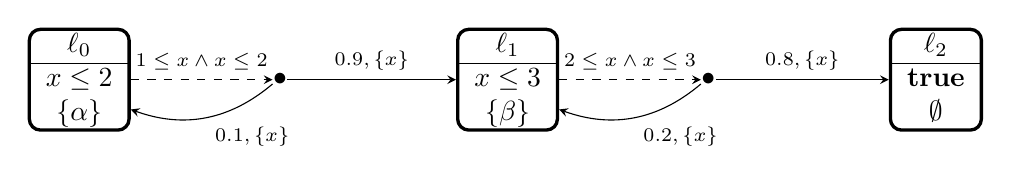
\begin{tikzpicture}[x = 1.7cm]
\node[location] (task1)         at (0,0)
{
\begin{tabular}{c}
$\loc_0$\\
\hline
$x\le 2$ \\
$\{\alpha\}$
\end{tabular}
};

\node[dec] (dec1)                    at (1.5,0)  {$\bullet$};

\node[location] (task2)         at (3.2,0)
{
\begin{tabular}{c}
$\loc_1$\\
\hline
$x\le 3$ \\
$\{\beta\}$
\end{tabular}
};

\node[dec] (dec2)                    at (4.7,0)  {$\bullet$};

\node[location] (finished)         at (6.4,0)
{
\begin{tabular}{c}
$\loc_2$\\
\hline
$\true$ \\
$\emptyset$
\end{tabular}
};

\draw[tran,dashed]    (task1)    to node[auto, font=\scriptsize] {$1\le x\wedge x\le 2$}    (dec1);
\draw[tran,bend left] (dec1)     to node[auto, font=\scriptsize] {$0.1,\{x\}$}     (task1);
\draw[tran]           (dec1)     to node[auto, font=\scriptsize] {$0.9, \{x\}$}    (task2);
\draw[tran,dashed]    (task2)    to node[auto, font=\scriptsize] {$2\le x\wedge x\le 3$}     (dec2);
\draw[tran,bend left] (dec2)     to node[auto, font=\scriptsize] {$0.2,\{x\}$}     (task2);
\draw[tran]           (dec2)     to node[auto, font=\scriptsize] {$0.8, \{x\}$}    (finished);
\end{tikzpicture}
}
\caption{A Task-Completion Example}
\label{fig:taskcompletion}
\vspace{-1em}
\end{figure}

A simple specification for {\sc Task-Completion} problem is that all tasks should be finished within a given amount of time with probability at least some given number.
We consider DTA-specifications which can express also the maximal completion time over individual tasks.
Example~\ref{ex:taskcompletiondta} explains this idea.

\begin{example}\label{ex:taskcompletiondta}
Consider the DTA depicted in Figure~\ref{fig:dtataskcompletion} which works as a specification for the PTA in Example~\ref{ex:taskcompletion}.
$q_i$'s ($1\le i\le 4$) are modes with $q_3$ being the final mode, $y,z$ are clocks and arrows between modes are rules.
For example, there are two rules emitting from $q_1$, one is $(q_1, \{\beta\}, y\le 3, \{y\}, q_2)$ and the other is
$(q_1, \{\alpha\}, \true,\emptyset, q_1)$.
$q_0$ is the initial mode to read the label of the initial location of a PTA in the product construction, and
$q_3$ is the final mode.
Note that this DTA does not satisfy the totality condition. However, this can be remedied by adding rules leading to a deadlock mode without changing the acceptance behaviour of the DTA.
In the product construction with the PTA in Example~\ref{ex:taskcompletion}, $y$ records completion time of individual tasks and $z$ records completion time of both tasks.
The specification then says that the PTA should complete the first task in $3$ time units (by $y\le 3$), the second task in $4$ time units (by $y\le 4$), and all the tasks in $6$ time units (by $z\le 6$).\qed
\end{example}

\begin{figure}
\centering
\resizebox{.5\textwidth}{!}{
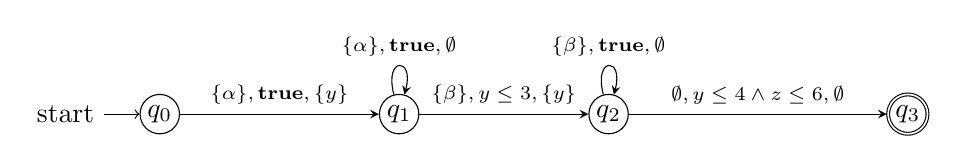
\begin{tikzpicture}[x = 3.8cm]
\node[mode,initial] (q0)         at (0.5,0)  {$\dtloc_0$};
\node[mode] (q1)         at (1.3,0)  {$\dtloc_1$};
\node[mode] (q2)         at (2,0)  {$\dtloc_2$};
\node[mode,accepting] (q3)         at (3,0)  {$\dtloc_3$};

\draw[tran] (q0)       to node[auto, font=\scriptsize] {$\{\alpha\}, \true, \{y\}$}      (q1);
\draw[tran, loop above] (q1)       to node[auto, font=\scriptsize] {$\{\alpha\}, \true, \emptyset$}  (q1);
\draw[tran] (q1)       to node[auto, font=\scriptsize] {$\{\beta\}, y\le 3,  \{y\}$} (q2);
\draw[tran, loop above] (q2)       to node[auto, font=\scriptsize] {$\{\beta\}, \true, \emptyset$}  (q2);
\draw[tran] (q2)       to node[auto, font=\scriptsize] {$\emptyset, y\le 4\wedge z\le 6,  \emptyset$} (q3);

\end{tikzpicture}
}
\caption{A DTA Specification for Example~\ref{ex:taskcompletion}}
\label{fig:dtataskcompletion}
\end{figure}
% \vspace{-0.8em}
\subsection{Robot Navigation}
% \vspace{-0.8em}
This case study is motivated from~\cite{DBLP:conf/tacas/BarbotCHKM11}.
In this case study, a robot is given the task to reach a destination in an unknown area.
Since the area is unknown,
the strategy the robot takes is to traverse the area randomly until the destination is reached.
Example~\ref{ex:robotnavigation} illustrates a simple setting on a $3$-by-$2$ grid.



\begin{example}\label{ex:robotnavigation}
Consider the robot-navigation problem depicted in Figure~\ref{fig:robotnavigation}.
On each tile, the time taken by a robot to leave the tile is always between $2$ and $3$ time-units.
The tile filled with black is an obstacle which cannot be entered.
The task for a robot is to start from the left-down corner of the $3$-by-$2$ grid, and move uniform-randomly to adjacent tiles excluding the obstacle until the upright corner is reached.
We assume that the robot does not always succeed to leave a tile, and the probability to successfully leave a tile is $0.9$.
The PTA modelling this problem is depicted in Figure~\ref{fig:ptarobotnavigation},
for which $x$ is the clock to measure the dwell-time on each tile, $\alpha,\beta$ are atomic propositions that distinguish adjacent tiles, and the way that the PTA is depicted is the same as for Example~\ref{ex:taskcompletion} and Figure~\ref{fig:taskcompletion}.
Each location $\loc_{i,j}$ corresponds to the situation that the robot stands in the tile $(i,j)$ (viewed as a coordinate in a two-dimensional plane) of the original grid.
The location $\loc_{2,1}$ is labelled $\emptyset$ to signify the destination.
Same as in Example~\ref{ex:taskcompletion}, we elaborate invariant conditions to disallow schedulers from repeatedly choosing time elapses. \qed
\end{example}

\begin{figure}
\begin{minipage}{0.3\textwidth}
\centering
~~\\
~\\
~\\
\scalebox{0.8}[0.8]{
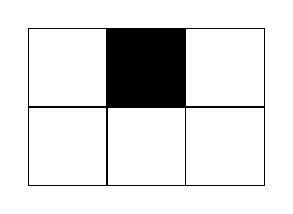
\begin{tikzpicture}[x = 1cm]
\begin{scope}
    \draw (0, 1) grid (3, 3);

    \setcounter{row}{1}
    \setrow{}{}{}
    \setrow{}{}{}
%    \node[anchor=center] at (1.5, -0.5) {Robot Navigation};
\end{scope}

\fill[black] (1,2) rectangle (2,3);

\end{tikzpicture}
}
\caption{A Robot Navigation}
\label{fig:robotnavigation}
\end{minipage}
\begin{minipage}{0.6\textwidth}
\centering
\scalebox{0.5}[0.5]{
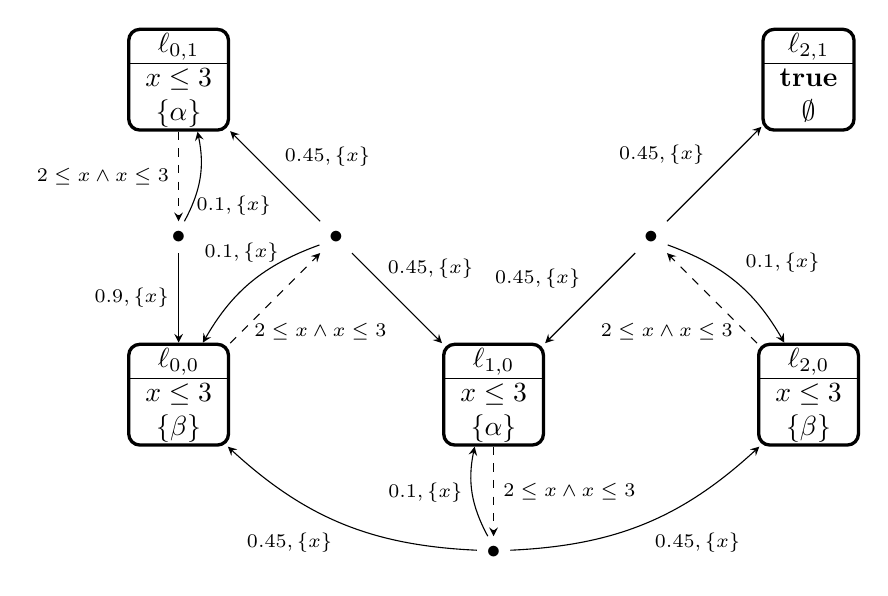
\begin{tikzpicture}[x=2cm, y=2cm]

\node[location] (q00)         at (0,0)
{
\begin{tabular}{c}
$\loc_{0,0}$\\
\hline
$x\le 3$ \\
$\{\beta\}$
\end{tabular}
};

\node           (dec00)       at (1, 1) {$\bullet$};

\node[location] (q01)         at (0,2)
{
\begin{tabular}{c}
$\loc_{0,1}$\\
\hline
$x\le 3$ \\
$\{\alpha\}$
\end{tabular}
};

\node           (dec01)       at (0, 1) {$\bullet$};

\node[location] (q10)         at (2,0)
{
\begin{tabular}{c}
$\loc_{1,0}$\\
\hline
$x\le 3$ \\
$\{\alpha\}$
\end{tabular}
};

\node (dec10) at (2,-1) {$\bullet$};

\node[location] (q20)         at (4,0)
{
\begin{tabular}{c}
$\loc_{2,0}$\\
\hline
$x\le 3$ \\
$\{\beta\}$
\end{tabular}
};

\node (dec20)  at (3,1) {$\bullet$};

\node[location] (q21)         at (4,2)
{
\begin{tabular}{c}
$\loc_{2,1}$\\
\hline
$\true$ \\
$\emptyset$
\end{tabular}
};

\node (sp1) at (0.9,0.4)  {{\scriptsize $2\le x\wedge x\le 3$}};
\node (sp2) at (3.1,0.4)  {{\scriptsize $2\le x\wedge x\le 3$}};
\node (dec00q00) at (0.4,0.9)  {{\scriptsize $0.1, \{x\}$}};
\node (dec01q01) at (0.35, 1.2)  {{\scriptsize $0.1, \{x\}$}};
\node (dec00q10) at (1.6, 0.8) {{\scriptsize $0.45, \{x\}$}};

%\node (dec21)  at (4,1) {$\bullet$};

\draw[tran]               (dec00)       to node[above right, font=\scriptsize]  {$0.45, \{x\}$}     (q01);
\draw[tran]               (dec00)       to      (q10);
\draw[tran,bend right=20] (dec00)       to      (q00);

\draw[tran]               (dec01)       to node[left, font=\scriptsize]  {$0.9, \{x\}$}               (q00);
\draw[tran,bend right=20] (dec01)       to                (q01);

\draw[tran,bend left=20]   (dec10)       to node[below left, font=\scriptsize]  {$0.45, \{x\}$}             (q00);
\draw[tran,bend right=20]  (dec10)       to node[below right, font=\scriptsize]  {$0.45, \{x\}$}             (q20);
\draw[tran,bend left=20]   (dec10)       to node[left, font=\scriptsize]  {$0.1, \{x\}$}           (q10);

\draw[tran]  (dec20)       to node[above left, font=\scriptsize]  {$0.45, \{x\}$}     (q10);
\draw[tran]  (dec20)       to node[auto, font=\scriptsize]  {$0.45, \{x\}$}     (q21);
\draw[tran, bend left=20]  (dec20)       to node[auto, font=\scriptsize]  {$0.1, \{x\}$}     (q20);

\draw[tran, dashed]  (q00)  to   (dec00);
\draw[tran, dashed]  (q01)  to node[left, font=\scriptsize]  {$2\le x\wedge x\le 3$}  (dec01);
\draw[tran, dashed]  (q10)  to node[auto, font=\scriptsize]  {$2\le x\wedge x\le 3$}  (dec10);
%\draw[tran, dashed]  (q21)  to node[auto, font=\scriptsize]  {$1\le x\wedge x\le 2$}  (dec21);
\draw[tran, dashed]  (q20)  to   (dec20);

\end{tikzpicture}
}
\caption{The PTA for Example~\ref{ex:robotnavigation}}
\label{fig:ptarobotnavigation}
\end{minipage}
\end{figure}



\begin{figure}
\centering
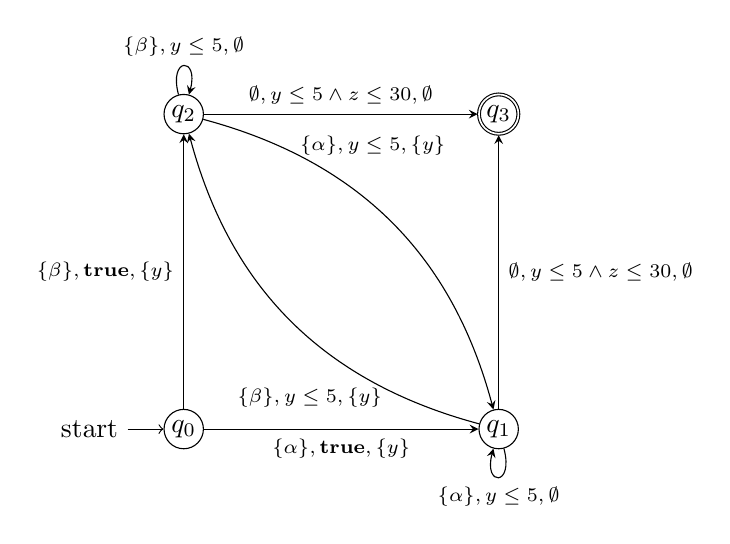
\begin{tikzpicture}[x = 4cm, y=4cm]

\node[mode,initial] (q0)         at (0,0)  {$\dtloc_0$};
\node[mode] (q1)         at (1,0)  {$\dtloc_1$};
\node[mode] (q2)         at (0,1)  {$\dtloc_2$};
\node[mode,accepting] (q3)         at (1,1)  {$\dtloc_3$};

\node (sp1) at (0.4, 0.1)  {{\scriptsize $\{\beta\}, y\le 5, \{y\}$}};
\node (sp2) at (0.6, 0.9) {{\scriptsize $\{\alpha\}, y\le 5, \{y\}$}};

\draw[tran] (q0)       to node[below, font=\scriptsize] {$\{\alpha\}, \true, \{y\}$}      (q1);
\draw[tran] (q0)       to node[left, font=\scriptsize] {$\{\beta\}, \true, \{y\}$}      (q2);
\draw[tran, loop below] (q1)      to node[auto, font=\scriptsize] {$\{\alpha\}, y\le 5, \emptyset$}  (q1);
\draw[tran, bend left]  (q1)      to    (q2);
\draw[tran, loop above] (q2)      to node[auto, font=\scriptsize] {$\{\beta\}, y\le 5, \emptyset$}   (q2);
\draw[tran, bend left]  (q2)       to    (q1);
\draw[tran] (q1)       to node[right, font=\scriptsize] {$\emptyset, y\le 5\wedge z\le 30,  \emptyset$} (q3);
\draw[tran] (q2)       to node[above, font=\scriptsize] {$\emptyset, y\le 5\wedge z\le 30,  \emptyset$} (q3);

\end{tikzpicture}
\caption{A DTA Specification for Example~\ref{ex:robotnavigation}}
\label{fig:dtarobotnavigation}
\end{figure}

Similar to the previous case study, we consider the specification that stress timing constraints on both dwell-time in individual tiles and total time to reach the destination for the robot.
\vspace{-0.5em}
\begin{example}
The DTA depicted in Figure~\ref{fig:dtarobotnavigation} specifies a property for the robot navigation described in Example~\ref{ex:robotnavigation}.
The way to render this DTA is the same as for Example~\ref{ex:taskcompletiondta}.
$q_0$ is the initial mode which reads the label of the initial tile where the robot lies and $q_3$ is the final mode.
The clock $y$ measures dwell-time on an individual tile, and the clock $z$ measures the total time to destination.
The property says that the robot should (i) never dwell on an individual tile more than $5$ time units (cf. the clock constraint $y\le 5$ and atomic propositions $\alpha,\beta$ that distinguishes adjacent tiles), and (ii) reach the upright corner within 30 time units (cf. the clock constraint $z\le 30$).\qed
\end{example}
\vspace{-0.8em}

\section{Experiments}\label{sec:experiments}
We validate our approach using multiple datasets containing real-life data from the fields of criminal risk assessment, credit, lending, and college admissions. In each of the datasets we select a binary feature and treat it as the protected attribute (e.g., race or gender), which is the feature we require our trained classifier to behave fairly upon. Our proposed method performs well on all of these datasets, succeeding in removing unfairness almost entirely, at a very modest price in terms of accuracy.


\begin{table*}[h]
\centering
\resizebox{\textwidth}{!}{
\def\arraystretch{1.2}

\begin{tabular}{c c c | c | c | c || c | c | c || c | c | c |}

\cline{4-12}
&&&
\multicolumn{9}{ c| }{\textbf{COMPAS Dataset}}
\\ \cline{4-12}
&&&
\multicolumn{3}{ c|| }{\textbf{FPR Considerations}}&
\multicolumn{3}{ c|| }{\textbf{FNR Considerations}}&
\multicolumn{3}{ c| }{\textbf{Both Considerations}}
\\ \cline{4-12}
&&&
 $\mathbf{Acc.}$ &  $\mathbf{D_{FPR}}$ &  $\mathbf{D_{FNR}}$ &  $\mathbf{Acc.}$ &  $\mathbf{D_{FPR}}$ &  $\mathbf{D_{FNR}}$ &  $\mathbf{Acc.}$ &  $\mathbf{D_{FPR}}$ &  $\mathbf{D_{FNR}}$
\\  \cline{4-12}
\vspace*{-0.5ex}
\\ \cline{1-2} \cline{4-12}
\multicolumn{1}{ |c  }{} &
\multicolumn{1}{ c|  }{  \textbf{Our Method (AVD Penalizers)}}  &&
$\mathbf{0.660}$    &  $\mathbf{0.01}$  &  $0.04$ &
$\mathbf{0.653}$    &  $0.02$   &  $\mathbf{0.04}$ &
$\mathbf{0.654}$    &  $\mathbf{0.02}$  &  $\mathbf{0.04}$
\\ \cline{1-2} \cline{4-12}
\multicolumn{1}{ |c  }{} &
\multicolumn{1}{ c|  }{  \textbf{Our Method (SD Penalizers)}}  &&
$\mathbf{0.664}$    &  $\mathbf{0.02}$  &  $0.09$ &
$\mathbf{0.661}$    &  $0.05$   &  $\mathbf{0.03}$ &
$\mathbf{0.661}$    &  $\mathbf{0.02}$  &  $\mathbf{0.03}$
\\ \cline{1-2} \cline{4-12}
\multicolumn{1}{ |c  }{} &
\multicolumn{1}{ c|  }{  Zafar et al.~(\citeyear{disparatemistreatment})}  &&
$0.660$    &   $0.06$    &   $0.14$  &
$0.662$    &   $0.03$    &   $0.10$  &
$0.661$    &   $0.03$    &   $0.11$
\\ \cline{1-2} \cline{4-12}
\multicolumn{1}{ |c  }{} &
\multicolumn{1}{ c|  }{  Zafar et al. Baseline~(\citeyear{disparatemistreatment})}  &&
$0.643$    &   $0.03$    &   $0.11$  &
$0.660$    &   $0.00$    &   $0.07$  &
$0.660$    &   $0.01$    &   $0.09$
\\ \cline{1-2} \cline{4-12}
\multicolumn{1}{ |c  }{} &
\multicolumn{1}{ c|  }{  Hardt et al.~(\citeyear{hardt})}  &&
$0.659$    &  $0.02$    &   $0.08$  &
$0.653$    &  $0.06$   &    $0.01$  &
$0.645$    &  $0.01$   &    $0.01$
\\ \cline{1-2} \cline{4-12}
\multicolumn{1}{ |c  }{} &
\multicolumn{1}{ c|  }{  \textbf{Vanilla Regularized Logistic Regression}}  &&
$\mathbf{0.672}$    &   $\mathbf{0.20}$    &   $\mathbf{0.30}$  &
$\mathbf{0.672}$    &   $\mathbf{0.20}$    &   $\mathbf{0.30}$  &
$\mathbf{0.672}$    &   $\mathbf{0.20}$    &   $\mathbf{0.30}$
\\ \cline{1-2} \cline{4-12}
\end{tabular}
}
\vspace{3mm}
\caption{Performance comparison on the COMPAS dataset. For the approaches in bold -- Accuracy, FPR difference and FNR difference are evaluated on the test set, averaging over five runs and using a 70-30 training/test split. The performance of the remaining three approaches is stated as reported in Zafar et al.~(\citeyear{disparatemistreatment}).} \label{table:comparison_results}
\end{table*}



\begin{figure*}[b]
  \includegraphics[scale=0.6]{compas0-400.png}
  \caption{COMPAS Dataset. Accuracy, FPR difference ($\mathbf{D_{FPR}}$), and FNR difference ($\mathbf{D_{FNR}}$) (all evaluated on the test set) of the learned classifier, as a function of the weight $c=c_1 = c_2 \geq 0$ placed on the fairness penalizer terms. On the left we use the Absolute Value Difference (AVD) penalizer, and the Squared Difference (SD) penalizer on the right, both as presented in Section~\ref{regularization}. ``Relaxed FPR/FNR Diff.'' plots the value of the relevant penalization term.} %In this particular run, parameters chosen for the absolute value relaxation were: $c=80, q_c=60$, and for the squared relaxation: $c=220, q_c=30$.}
  \label{fig:compas}
\end{figure*}


\subsection{Implementation}
\textbf{Our method} 
%We instantiate our method in the following way: Given dataset $Q$, we split it randomly into a training set $S$ (which we will use for learning) and a test set $T$ (which we will only use for reporting performance). 
For the purpose of comparison with  Zafar et al.~(\citeyear{disparatemistreatment}) and Hardt et al.~\cite{hardt} on the COMPAS data, we use a parameter $c$ to induce three possible combinations of weights on the FPR and FNR penalization terms: $c = c_1$ and $c_2 = 0$; $c_1 = 0$ and $c = c_2$; and $c = c_1 = c_2$. For the other three datasets, we consider only $c = c_1 = c_2$.\footnote{The reason for varying the values of $c$ in the training phase is since we shifted to a proxy problem, in which we rely on the distance from the decision boundary rather the actual classifications. 
%Our hope is that there is no need for a worst-case cross validation between all of the combinations of $c_1, c_2, c_3$, and that the training scheme we propose is sufficient. 
It is possible, of course, that even better results are attainable using our scheme with other combinations of $c_1, c_2$, and $q$.} To explore the accuracy/fairness trade-off curve for the relaxed optimization problem~(\ref{eq:2}), we train for different values of $c$, starting at $c=0$ (which is just standard logistic regression), and growing gradually.



Given a dataset $Q$ and fixing a $d_1, d_2 \in \{0, 1\}$ of interest, we use the following training scheme:
\begin{enumerate}
\item Split $Q$ at random into training set $S$ and test set $T$.
\item For each $c$, perform cross-validation on $S$ to select the corresponding best value $q_c$ for the regularization parameter.
\item For each $(c,q_c)$, let $\theta_c = \argmin\limits_{\theta} \text{Proxy}(\theta;S,c,c,q_c)$.
\item Select $\theta^* \in \argmin\limits_{\theta_c} \text{Objective}(\theta_c;S,d_1,d_2)$.
\item Evaluate performance using $\theta^*$ on test set $T$.
\end{enumerate}
We report the average of five such runs, each with a fresh training-test split.




%We instantiate our method by solving the relaxed optimization problem~(\ref{eq:2}), in place of the original, non-convex problem~(\ref{eq:1}).  
%We test our approach with three different combinations of weights on the penalization terms:
%\katrina{What are the $d$, and how are they related to the $c$s?}
%\begin{enumerate}
%\item FPR considerations only: $d_1 = 1, d_2 = 0$.
%\item FNR considerations only: $d_1 = 0, d_2 = 1$.
%\item Both FPR, FNR considerations, assigned similar significance: $d_1 = 1, d_2 = 1$.
%\end{enumerate}
%One could, of course, pick any other combination of the FPR and FNR penalty weights.

%\katrina{I don't understand how the below is distinct from the list above}
%Learning is done by training the parameters of a logistic regressor to solve~\ref{eq:2}, while picking the value of $c_1, %c_2$ as the following:
%\begin{enumerate}
%\item FPR considerations only: $c_1 = c \geq 0$, $c_2 = 0$.
%\item FNR considerations only: $c_1 = 0$, $c_2 = c \geq 0$.
%\item Both FPR, FNR considerations, assigned similar significance: $c_1 = c_2 = c \geq 0$
%\end{enumerate}



% We then cross-validate to pick the best $c_3$ (the weight on the standard $\ell_2$-regularization term) given $c$.\footnote{The reason for varying the values of $c$ in the training phase is since we shifted to a proxy problem, in which we rely on the distance from the decision boundary rather the actual classifications. 
%Our hope is that there is no need for a worst-case cross validation between all of the combinations of $c_1, c_2, c_3$, and that the training scheme we propose is sufficient. 
%It is possible, of course, that even better results are attainable using our scheme with other combinations of $c_1, c_2, c_3$.} For each such combination, we report results as the averages of multiple \katrina{how many?} different runs, each time splitting data randomly into training and test sets.
%\yahav{We need to shorten this description.}

We solve the relaxed convex optimization problem using the CVXPY solver. Due to stability issues with large training sets, we use a train/test split of 30-70 on the larger datasets, rather than 70-30 as on the COMPAS dataset\footnote{The code implementing our method can be found at https://github.com/jjgold012/lab-project-fairness}.

%
%
%We then report the results (as evaluated on the test set) attained by a regressor $\theta \in \mathbb{R}^d$ that minimizes (on the training set $S$) a weighted combination of the $0$-$1$ loss and the differences in FPR and FNR across populations:
%\begin{equation*}
%\begin{aligned}
%&\underset{\theta}{\text{argmin}}
%& & L_{S}^{0\text{-}1}(\theta) \\
%&&& + d_1|FPR_{A=0}(\theta;S)-FPR_{A=1}(\theta;S)| \\
%&&& + d_2|FNR_{A=0}(\theta;S)-FNR_{A=1}(\theta;S)|
%\end{aligned}
%\end{equation*}
%
%\katrina{What is $d_1$ vs. $c_1$ etc.?}



%For classification, we decided use a standard cut-off threshold of $c=0.5$. There are of course, further possible interactions between the FPR, FNR considerations, and picking a certain cut-off level. These are not straightforward, since  these interactions are data-specific. 



%allows for flexibility in picking the values of $c_1, c_2$, which reflect the significance we wish to place on the objectives of achieving accuracy, equal FPR, and equal FNR. As for $c_3$, we will want to find the value of it that achieves the best results, for any combined objective of accuracy and fairness defined by a specific selection of $c_1,c_2$. Therefore, given a specific selection of $c_1, c_2$, we apply cross-validation to select the value of $c_3$. 




We briefly describe the other algorithmic approaches to which we compare:\\
\textbf{Zafar et al.}~(\citeyear{disparatemistreatment}) performs optimization by considering a proxy for the bias: the covariance between the samples' sensitive attributes and the signed distance between the feature vectors of misclassified users and the classifier decision boundary.\\
\textbf{Zafar et al. Baseline}~(\citeyear{disparatemistreatment}) tries to enforce equal FP/FN rates on the different groups by introducing different penalties for misclassified data points with different sensitive attribute values during the training phase.\\
\textbf{Hardt et al.}~(\citeyear{hardt}) performs post-processing on a standard trained (unfair) logistic regressor, picking different decision thresholds for different groups, and possibly adding randomization.


\subsection{Experimental Results}

In what follows, we use the following notation, given a trained classifier $\hat{Y}$:
\begin{align*}
\mathbf{D_{FPR}}&=\left|FPR_{A=0}(\hat{Y})-FPR_{A=1}(\hat{Y})\right| \\ 
\mathbf{D_{FNR}}&=\left|FNR_{A=0}(\hat{Y})-FNR_{A=1}(\hat{Y})\right|
\end{align*}
The values $FPR_{A=0}(\hat{Y})$, $FPR_{A=1}(\hat{Y})$, $FNR_{A=0}(\hat{Y})$, $FNR_{A=1}(\hat{Y})$ are reported as evaluated on the test set.

\paragraph{The COMPAS Dataset\footnote{https://github.com/propublica/compas-analysis}} The Correctional Offender Management Profiling for Alternative Sanctions (COMPAS) records from Broward County, Florida 2013-2014, made available online by ProPublica, are perhaps the best-studied data in the context of fairness.  The goal in this scenario is to successfully predict recidivism within two years, based on features such as age, gender, race, number of prior offenses, and charge degree. The dataset contains 5,278 samples. The protected attribute in this scenario is race, where $A$ indicates black or white. We filtered the dataset using the same features as Zafar et al.~(\citeyear{disparatemistreatment}), to allow for comparison.

%\begin{table}[h]
%\centering
%\begin{tabularx}{\columnwidth}{c|c|c|c}
%\hline
%  &  Recid. ($y = 1$)        & No Recid.  ($y = 0$)       & Total \\ \hline
%Black &  $ 1661   $ & $ 1514 $ &  $ 3175 $ \\ \hline
%White &  $ 822   $  & $1281  $ &  $ 2103 $ \\ \hline
%Total &  $ 2483  $  & $2795 $ &  $ 5278 $ \\\hline
%\end{tabularx}
%\caption{Statistics of the ProPublica COMPAS data.} \label{table:compas-stats}
%\label{tab:stats}
%\end{table}
%\vspace{-1em}

%\begin{table}[h]
%\centering
%\begin{tabularx}{\columnwidth}{c|c}
%\hline
%Feature  &  Description \\ \hline
%Age Category &  $<25$, between $25$ and $45$, $>45$ \\
%Gender &  Male or Female \\
%Race &  White or Black \\
%Priors Count &  0--37 \\
%Charge Degree &  Misconduct or Felony \\
%\hline
%2-year-recid. & Whether or not the  \\
%(target feature)  & defendant recidivated within two years
%\end{tabularx}
%\caption{Description of features used from ProPublica COMPAS data.} \label{table:compas-features}
%\label{tab:features}
%\end{table}




\begin{table*}[t]
\centering
\caption{A description of the datasets used, along with parameters of the training procedure used for each.}
\label{table:datasets_description}
\begin{adjustbox}{max width=\textwidth}
\begin{tabular}{|l|l|l|l|l|l|l|l|}
\hline
\textbf{Dataset} & \textbf{No. Samples} & \textbf{No. Features} & \textbf{Train/Test Split} & \textbf{No. Repetitions} & \textbf{No. Folds in CV} & \textbf{Protected Feature} & \textbf{Target Variable} \\ \hline
COMPAS           & 5,278                     & 5                          & 70-30                     & 5                        & 5                                 & Race                       & 2-Year-Recidivism        \\ \hline
Adult            & 30,162                    & 10                         & 30-70                     & 5                        & 5                                 & Gender                     & Income Over/Under 50K    \\ \hline
Default          & 30,000                    & 23                         & 30-70                     & 5                        & 3                                 & Gender                     & Defaulting On Payments   \\ \hline
Admissions       & 20,839                    & 17                         & 30-70                     & 5                        & 3                                 & Race                       & Passing Bar Exam         \\ \hline
\end{tabular}
\end{adjustbox}
\end{table*}


\begin{table*}[t]
\centering
\resizebox{\textwidth}{!}{
\def\arraystretch{1.2}

\begin{tabular}{c c c | c | c | c || c | c | c || c | c | c |}

\cline{4-12}
&&&
\multicolumn{3}{ c|| }{\textbf{Adult Dataset}}&
\multicolumn{3}{ c|| }{\textbf{Default Dataset}}&
\multicolumn{3}{ c| }{\textbf{Admissions Dataset}}
\\ \cline{4-12}
%&&&
%\multicolumn{3}{ c|| }{\textbf{Both Considerations}}&
%\multicolumn{3}{ c|| }{\textbf{Both Considerations}}&
%\multicolumn{3}{ c| }{\textbf{Both Considerations}}
%\\ \cline{4-12}
&&&
 $\mathbf{Acc.}$ &  $\mathbf{D_{FPR}}$ &  $\mathbf{D_{FNR}}$ &  $\mathbf{Acc.}$ &  $\mathbf{D_{FPR}}$ &  $\mathbf{D_{FNR}}$ &  $\mathbf{Acc.}$ &  $\mathbf{D_{FPR}}$ &  $\mathbf{D_{FNR}}$
\\  \cline{4-12}
\vspace*{-0.5ex}
\\ \cline{1-2} \cline{4-12}
\multicolumn{1}{ |c  }{} &
\multicolumn{1}{ c|  }{  \textbf{Our Method (AVD Penalizers)}}  &&
$\mathbf{0.776}$    &  $\mathbf{0.00}$  &  $\mathbf{0.04}$ &
$\mathbf{0.807}$    &  $\mathbf{0.00}$   &  $\mathbf{0.01}$ &
$\mathbf{0.950}$    &  $\mathbf{0.01}$  &  $\mathbf{0.00}$
\\ \cline{1-2} \cline{4-12}
\multicolumn{1}{ |c  }{} &
\multicolumn{1}{ c|  }{  \textbf{Our Method (SD Penalizers)}}  &&
$\mathbf{0.783}$    &  $\mathbf{0.00}$  &  $\mathbf{0.09}$ &
$\mathbf{0.806}$    &  $\mathbf{0.01}$   &  $\mathbf{0.02}$ &
$\mathbf{0.950}$    &  $\mathbf{0.00}$  &  $\mathbf{0.00}$
\\ \cline{1-2} \cline{4-12}
\multicolumn{1}{ |c  }{} &
\multicolumn{1}{ c|  }{  \textbf{Vanilla Regularized Logistic Regression}}  &&
$\mathbf{0.800}$    &   $\mathbf{0.08}$    &   $\mathbf{0.39}$  &
$\mathbf{0.807}$    &   $\mathbf{0.01}$    &   $\mathbf{0.05}$  &
$\mathbf{0.951}$    &   $\mathbf{0.16}$    &   $\mathbf{0.02}$
\\ \cline{1-2} \cline{4-12}
\end{tabular}
}
\vspace{3mm}
\caption{Performance on the Adult, Loan Default, and Admissions datasets, penalizing for both FPR and FNR difference. Accuracy, FPR difference and FNR difference are evaluated on the test set, averaging over five runs and using a 30-70 training/test split.} \label{table:comparison_results_rest}
\end{table*}


In Table~\ref{table:comparison_results}, we compare the performance of our approach with that of three other techniques from the literature. Each method was trained based on logistic regression.  As a basis for comparison, we also present the performance of vanilla logistic regression, absent fairness considerations, with the regularization parameter selected via cross-validation.\footnote{Zafar et al.~(\citeyear{disparatemistreatment}) do not incorporate regularization in any of the approaches they report.}
%Results are reported as the averages of 5 different runs \katrina{Is that still correct?}, each time splitting data evenly and randomly into training and test sets. 
Results for Zafar et al., Zafar et al. baseline, and Hardt et al. appear here as reported in Zafar et al.~(\citeyear{disparatemistreatment}).\footnote{Our method selects the classifier based on the training set only and reports its performance over the test set. Results for the three other approaches, reported by Zafar et al.~(\citeyear{disparatemistreatment}), are based on tuning parameters after seeing the trade-off curve over the test set, and reporting according to the best selection of these parameters.}
%\katrina{Perhaps here is the right place for a footnote about the discrepancy with the Zafar baseline}

We find that the vanilla logistic regressor (absent fairness considerations) results in significant unfairness, as $\mathbf{D_{FPR}}=0.20$, and $\mathbf{D_{FNR}}=0.30$. The overall accuracy of this classifier measured on the test set was $0.672$.\footnote{Zafar et al.~(\citeyear{disparatemistreatment}) report a slightly different baseline of: Accuracy = 0.668, $\mathbf{D_{FPR}}=0.18$, $\mathbf{D_{FNR}}=0.30$.} Our SD penalization approach empirically achieves approximately the same accuracy as the Zafar et al.~(\citeyear{disparatemistreatment}) approach, with significantly better fairness. It is difficult to compare fairness-accuracy tradeoffs with the Hardt et al.~(\citeyear{hardt}) approach, since their accuracy is significantly lower than ours. A more direct comparison is possible by noting that our learned classifier can be post-processed to improve its fairness at a direct cost to accuracy. Hence, we can achieve accuracy of $0.659$ with $\mathbf{D_{FPR}} = \mathbf{D_{FNR}} = 0.01$, which compares very favorably with the Hardt et al. accuracy rate of 0.645 given the same FPR and FNR rates.\footnote{For completeness, we note that using a 50-50 training-test split (again not using the test set for parameter selection), our method (SD, both considerations) produces a classifier that provides: Accuracy = 0.659, $\mathbf{D_{FPR}} = 0.01, \mathbf{D_{FNR}} = 0.05$. This classifier can be post-processed to achieve rates of: Accuracy = 0.655, $\mathbf{D_{FPR}} = \mathbf{D_{FNR}} = 0.01$.}

Figure \ref{fig:compas} illustrates the accuracy/fairness trade-offs achievable using our scheme. Increasing the weight $c$ on the proxy fairness penalizers results in reducing their magnitude. The figure also illustrates how our relaxed penalizers succeed in tracking the real FPR and FNR differences. 
%
%
%\katrina{Must rewrite the following paragraph}
%We observe that our method succeeds in eliminating unfairness almost completely on the COMPAS dataset, while retaining most of the accuracy, when compared to the vanilla logistic regression. We achieve very low difference rates when penalizing for achieving each of the FPR and FNR criteria individually, and also for both. We achieve preferable results comparing to Zafar et al. and Zafar et al. baseline in all 3 scenarios, and also comparing to Hardt et al. in the settings of false positive/false negative considerations only. In the setting of both considerations - The Hardt et al. method removes a larger portion of the unfairness, however it results in major accuracy loss as it achieves accuracy rate of 0.645 in comparison to our method which results in accuracy of 0.665, retaining most of the original accuracy rate while removing most of the unfairness.




%The Hardt et al.~\cite{hardt} approach as reported removes a smaller portion of the bias in the different scenarios, however for FP/FN constraints alone, it provides higher accuracy rates. The Zafar et al.~(\citeyear{disparatemistreatment}) approach as reported retains significant bias (in most cases), but in some cases  achieves slightly superior accuracy rates to the methods above. 

%These performance comparisons are incomplete in the sense that each of the compared techniques has the potential to trade off between accuracy and fairness, using some degree of parameter tuning; what we report here is only one point on the achievable trade-off frontier for each algorithm. The ``correct'' trade-off, and, in particular, the best manner in which to weigh unfairness in the FPR against unfairness in the FNR, are matters of opinion. We have chosen to report our method's performance under parameters designed to very aggressively mitigate unfairness, at some cost to the accuracy.

%It would certainly be desirable to evaluate these and other approaches to fair learning on other datasets and on different tasks, particularly on larger datasets, which might afford both greater accuracy and better bias-reduction. The present empirical evaluations, however, suggest that our regularization-based approach provides a new tool worthy of consideration---we succeed in almost entirely eliminating bias on the hold-out set, at a modest price in terms of accuracy.

%Due to the fact that our true objective includes the original non-convex penalization terms, our approach does not carry any formal guarantees. However, the ease of implementation, generality, and empirical results are encouraging. Figure~\ref{fig:test1} illustrates the rate of convergence to a fair, accurate classifier on this dataset.
%In terms of computation costs, given that at each iteration we must calculate the gradient according to the FPR and FNR regularizers, we are required to predict the labels for the entire training set at each step. 
%However, this does not pose a computational burden, as it is already required by the (classic) gradient descent algorithm in our logistic regressor fitting scheme. Furthermore, when given a sufficiently large dataset (one or two orders of magnitude larger than the one currently available for the COMPAS scores data), this could be relaxed to sampling only a mini-batch of samples from the training data set at each iteration (much as is done in stochastic gradient descent).






\subsection{Additional Datasets}


Table~\ref{table:datasets_description} provides summary statistics on each of the datasets on which we tested our approach. We also briefly describe the datasets below. 


{\bf The Adult Dataset}\footnote{http://archive.ics.uci.edu/ml/datasets/Adult} is based on 1994 US Census data. The task we consider is to predict whether the income of each individual is over or under 50K dollars per year, based on features such as occupation, marital status, and education. The protected attribute selected in this task is gender. 

{\bf The Loan Default Dataset}\footnote{{\scriptsize https://archive.ics.uci.edu/ml/datasets/default+of+credit+card+clients}}
contains data regrading Taiwanese credit card users. The task we consider is to predict whether an individual will default on payments, based on features such as history of past payments, age, and the amount of given credit. The protected attribute is gender.

{\bf The Admissions Dataset}\footnote{http://www2.law.ucla.edu/sander/Systemic/Data.htm}
contains records of law school students who went on to take the bar exam. The task we consider is to predict whether a student will pass the exam based on features such as LSAT score, undergraduate GPA, and family income. The protected attribute is set to race.

Table~\ref{table:comparison_results_rest} describes the performance of our approach on these datasets, and Figures~\ref{fig:adult},~\ref{fig:default}, and~\ref{fig:lawschool} illustrate the fairness-accuracy trade-offs we achieve in each context. Overall, we see that unfairness is nearly eliminated while accuracy remains quite high. The dataset on which accuracy suffers most under our approach is the Adult dataset, which is also the dataset on which the vanilla regression is the most unfair.


\begin{figure*}[]
  \includegraphics[scale=0.6]{adult0-800.png}
  \caption{Adult Dataset. Fairness-Accuracy tradeoffs, as in Figure~\ref{fig:compas}.}
  \label{fig:adult}  
\end{figure*}



\begin{figure*}[]
  \includegraphics[scale=0.6]{default0-50.png}
  \caption{Loan Default Dataset. Fairness-Accuracy tradeoffs, as in Figure~\ref{fig:compas}.}
  \label{fig:default}
\end{figure*}



\begin{figure*}[]
  \includegraphics[scale=0.6]{admissions0-400.png}
  \caption{Admissions Dataset. Fairness-Accuracy tradeoffs, as in Figure~\ref{fig:compas}.}
  \label{fig:lawschool}
\end{figure*}



% \newcommand{\idx}[1]{\mbox{\sl index}
    \left (
        {#1}
    \right )
}

% \newcommand{\succe}[2]{
%     \mbox{\sl succ} \left(
%         {#1},
%         {#2}
%     \right)
% }
\newcommand{\successor}{
    \mbox{\sl succ} 
}
\vspace{-0.8em}
\section{Infinite-State-MDP Construction}
\vspace{-0.8em}

% Now we present the finite acceptance of nodeterministic timed automata for PTAs.
% \vspace{-0.8em}
% \begin{definition}[Finite Acceptance Criterion]
% Let $F\subseteq\cstates$ be a set of \emph{final} modes.
% An infinite word $w$ is \emph{finitely accepted} by $\dta$ w.r.t the \emph{initial configuration} $(\dtloc,\nu)$ and $F$ if $\run{\dta}{\dtloc,\nu}{w}=\{(\dtloc_n,\nu_n,a_n)\}_{n\in\Nset_0}$ satisfies that $\dtloc_n\in F$ for
% some $n\in\Nset_0$.
% \end{definition}

% \begin{definition}[Path Acceptance]
% An infinite path $\infpath$ under $\pta$ is \emph{finitely accepted} by $\tra$ w.r.t 
% initial configuration $(\dtloc,\nu)$, if the infinite word $\lbfunc(\infpath)$ is finitely
% accepted by $\tra$ w.r.t 
% $
% \left(\trfunc\left((\dtloc,\nu), \lbfunc(\initloc{\infpath})\right),\zero\right)
% $.
% \end{definition}
% 
% \begin{definition}[floor Operator]
% For a region $\reg$ with clocks $\clocks$, $\floor{\reg} : \clocks \rightarrow \Nset$ 
% is defined as $ \floor{\reg}(x) = t $ where $t$ is the unique integer s.t. 
% $\reg \models t \le x < t+1$
% \end{definition}
% 
Below we fix a well-formed PTA $\pta$ taking the form (\ref{eq:pta}) and a TFA $\dta$ taking the form (\ref{eq:tfa}) with the difference that the set of clocks for $\pta$ (resp. for $\nta$) is denoted by $\clocksX$ (resp. $\clocksY$).
W.l.o.g., we assume that $\clocksX \cap \clocksY = \emptyset$ and $\alphabet=2^{\ap}$.

Let PTA be $\pta$ with the set $\clocksX$ and the TFA be $\nta$ with the set $\clocksY$.

The transformation to MDP is as follows.

Let $\clocksY$ be a fixed finite set of clocks. We use integer Subscript denote a set of 
new clocks. Formally
$
    \clocksY_k = \left \{
        \left (
            t,y
        \right ) \in \Nset \times \clocksY
        \mid
        t = k
    \right \}
$ for $ k > 0 $.
For convenience, we use $ \clocksY_0 $ denote $ \clocksX $.

And $\reg^{\clocksY_k}$ is a region for $\clocksY_k$.
\begin{definition}[Product Construction (Infinite-State-MDP)]
The \emph{product MDP} $\productmdp{\pta}{\dta_q}$ between $\pta$ and $\dta$ with initial mode $\dtloc$ is defined as the PTA

\newcommand{\clocksN}{
    \clocksX \cup \left(
        \bigcup_{k=1}^{n} \clocksY_k
    \right )
}

The transformation to MDP is follows. A state in $\productmdp{\pta}{\dta_q}$ 
is of the form 

\begin{equation}\label{eq:state0}
    \left (
        \loc
        ,
        \left (
            \dtloc_1,
            \cdots,
            \dtloc_n
        \right )
        ,
        \clocksALL
        ,
        \reg
    \right )
\end{equation}

where $n$ is an unbounded natural number, $\loc$ (w.r.t $\dtloc_i$) is a location in $\pta$ 
(w.r.t a mod in $\nta$) and $\reg$ is a region with clock names being $\clocksALL$.
The intuition is that 
$
\pair
    {\loc}
    {\project{\reg}{\clocksX}}
$ 
reflects the region for $\pta$,
$ 
\left (
    \pair
        {\dtloc_1}
        {\project{\reg}{\clocksY_1}}
    \cdots,
    \pair
        {\dtloc_n}
        {\project{\reg}{\clocksY_n}}
\right )
$
reflects a power set for $\nta$. An
\end{definition}
% 
% \begin{definition}[Consistency]
% A clock valuation $\nu$ is consistent with a state $\mdploc$ in the form of ~(\ref{eq:state0}), 
% denoted by $ \nu \in  \mdploc$
% iff $\nu \in \clocksN$, $ \nu \downarrow \clocksY_i \in \reg^{\clocksY_i} $ and 
% $\fracp{\nu(x)} < \fracp{\nu(y)}$ iff $x \subseteq y$ for all $x,y \in \clocksN$.
% \end{definition}
% 
\begin{definition}[Rename function]
Let $\clocksX$ and $\clocksY$ be two sets of clocks, $\nu$ is a clock valuation on $\clocksX$ and
$ f:\clocksX \leftrightarrow \clocksY $ is a rename function then $ \nu[f]=\nu \circ f^{-1} $.
% 
\end{definition}
\begin{lemma}
Let $\reg$ is a region with clock names $\clocksX$ and $X \subseteq \clocksX$,
$
    \project
        {\reg}
        {X}
$
is a region with clock names $X$.
\end{lemma}
\begin{definition}[Time successor]
A state
\begin{align*}
    \mdploc'
    =
    \left (
        \loc
        ,
        \left (
            \dtloc_1,
            \cdots,
            \dtloc_n
        \right )
        ,
        \clocksALL
        ,
        \reg'
    \right )
\end{align*}
is a time successor of $\mdploc$ in the form of ~(\ref{eq:state0}) where either 
\begin{compactitem}
    \item 
        $\mdploc = \mdploc'$ if 
        $
            \forall \nu \in \reg, t \in \Rset_{>0} : \nu + t \in \reg'
        $ or
    \item 
        $\reg'$ is another unique region if there exist a $ \nu \in \reg $ s.t.
        \begin{align*}
            \exists t \in \Rset_{\ge0} : (
                \nu + t \in \reg' 
                \land
                \forall t' \in [0,t] : \\ \left (
                    \left (
                        \nu + t' \in \reg \cup \reg'
                    \right )
                    \land
                    \nu + t' \models \inv(l)
                \right )
            )
        \end{align*}
\end{compactitem}
$ \successor $ is a binary relation, 
$
    \successor (
        \mdploc,
        \mdploc'
    )
$ iff $ \mdploc' $ 
is time successor of $ \mdploc $.
$ \successor $  can be seen as a function since every location has a unique time successor
and $ \successor^t(\mdploc) $ is the $t$ step time successor of $\mdploc$. 
\end{definition}

\begin{definition}[Transition relation]
$
    \acts_{\productmdp{\pta}{\dta_q}}
    =
    \acts \cup \Nset
$.
\end{definition}

\begin{definition}[Transition relation]

The \emph{transition relation} $\trans$ is the smallest relation such that the following two inference rules are satisfied : \\
(Delay)
$
    \begin{array}{cc}
        % \mdploc' \mbox{ is the time successor of } \mdploc \\
        \successor^{t} (
            \mdploc,
            \mdploc'
        )
        &
        t \in \Nset \\
        \hline
        \tran
            {\mdploc}
            {t}
            {\mu_{\mdploc'}}
        &
    \end{array}
$
\\
(Jump)
$
    \begin{array}{ccc}
        \nu \in \reg
        &
        % \tran
        %     {
        %         \pair
        %             {\loc}
        %             {\project{\nu}{\clocksX}}
        %     }
        %     {a}
        %     {\mu}
        \mu = \prob ( \loc, a)
        &
        \project{\nu}{\clocksX} \models \penab{\loc}{a}
        \\
        \hline
        &
        \tran
            {\mdploc}
            {a}
            {\mu^*}
        &
    \end{array}
$
\\
where, let 
\\
$$
\mdploc' =  \left (
    \loc'
    ,
    \left (
        \dtloc_{1_0}
        \cdots,
        % \dtloc_{1_{k_1}}
        % \cdots,
        \dtloc_{i_0}
        \cdots,
        \dtloc_{i_{k_i}}
        % \dtloc_{n_0}
        \cdots,
        \dtloc_{n_{k_n}}
        % \cdots,
    \right )
    ,
    \clocksX \cup \left(
        \bigcup_{i=1}^{n'} \bigcup_{j=0}^{k_i} \clocksY_{i_j}
    \right )
    ,
    \reg'
\right )
$$

\begin{align*}
    \mu^* \left (
       \mdploc'
    \right )
    = 
    \begin{cases}
        \mu(X,\loc')
        &
        \dag
        \\
        0
        & 
        \mbox{  otherwise }
    \end{cases}
\end{align*} 

${}^\dag$ The none zero case hold
$
    \mbox{ if } (
        \project
            {\reg'}
            {\clocksX}) 
        = 
        \evclass{
            \project
                {\nu}
                {\clocksX}
            [X := 0 ]
        }_\sim 
$, there exists
$
    \left (
        \dtloc_i,
        \lbfunc\left(\loc'\right),
        \phi,
        Y_{i_j},
        \dtloc_{i_j}
    \right) \in \rules
$ 
such that \\
$
    \project
        {\reg'}
        {\clocksY_{i_j}}
    = 
        \evclass{ \left (
                \project
                    {\nu} 
                    {\clocksY_{i}}
            \right) 
            [ Y_{i_j} := 0 ] 
            [ y \mapsto <i_j,y> ]
        }_\sim 
$ 
and 
$    
    \project
        {\reg}
        {\clocksY_{i}}
    \subseteq \sat{\phi}
$,
{\color{red} $ k_i $ is the number of successors of $ \dtloc_i $}. 

\end{definition}

\begin{definition}[Final states]
A state $\mdploc$ in the form of ~(\ref{eq:state0}) is a final state iff there exist 
$ 1 \le k \le n $ such that $\dtloc_k$ is a final state in TFA balabala.
\end{definition}
$
    \tran
        {\mdploc}
        {a}
        {\mdploc'}
$
holds iff there exist a transition
$
    \tran
        {\mdploc}
        {a}
        {\mu}
$
such that
$ \mdploc' \in \supp{\mu}$ .

Now we the Transformation for product MDP as
$
\pfunc :
% \cup
    \fnpaths{\pta}
    \cup
    \infpaths{\pta}
    \cup
\rightarrow 
% \cup
    \fnpaths{\product{\pta}{\dta_\dtloc}}
    \cup
    \infpaths{\productmdp{\pta}{\dta_q}}
$

For a finite path
\[
\fnpath=(\loc_0,\nu_0)a_0\dots a_{m-1}(\loc_m,\nu_m)
\]
under $\pta$ (note that $(\loc_0,\nu_0)=(\loc^*, \zero)$ by definition),
we define $\pfunc(\fnpath)$ to be the unique finite path
\begin{equation}
    \pfunc(\fnpath)
        :=
        \mdploc_0
        a'_0
        \dots 
        a'_{m-1}
        \mdploc_{m}
\end{equation}
where $\mdploc_i$ is in the form of 
\begin{equation}
    \left (
        \loc'_i
        ,
        \left (
            \dtloc_{i,1},
            \cdots,
            \dtloc_{i,n_i}
        \right )
        ,
        \clocksX \cup \left(
            \bigcup_{k=1}^{n_i} \clocksY_{i,k}
        \right )
        ,
        \reg_i
    \right )
\end{equation}
under $\productmdp{\pta}{\dta_\dtloc}$ such that (\dag)
\begin{compactitem}
\item   {\color{red}$ n_0 $ is the number of successors of $ \dtloc $.}
        $\dtatr
            {(\dtloc,\zero)}
            {\lbfunc(\loc^*)}
            {(q_i,\mu_i)}
        $ and
        % $\trfunc\left((\dtloc,\zero), \lbfunc(\loc^*)\right)=(q_i,\mu_i)$ } and 
        $ \mu_i \in \project{\reg_0}{\clocksY_{0,i}} $ 
        for all $ 0 \le i \le n_0 $, and
\item   for all $0\le k < m$, $\loc_k = \loc'_k$.
\item   for all $0\le k < m$, if $a_k\in [0,\infty)$, there exist an integer $a'_k=t$ 
        such that $\successor^t(s_{k},s_{k+1})$, $ \nu_{k} \in \project{\reg_{k}}{\clocksX} $ and 
        $ \nu_{k+1} \in \project{\reg_{k+1}}{\clocksX} $. If $t$ is not unique, let $t$ be the minimal one.
\item   for all $0\le k < m$, if $a_k\in\acts$ then $a'_{k}=a_k$ and 
$
    \tran
        {\mdploc_{k}}
        {a'_{k}}
        {\mdploc_{k+1}}
$.
\end{compactitem}
Likewise, we can define transformation for infinite paths.

We also show the relationship on schedulers before and after product construction.

\noindent{\textbf{Transformation $\sfunc$ From Schedulers under $\pta$ into Schedulers under $\productmdp{\pta}{\dta_q}$.}}
$ \sfunc(\sigma) $ follows $ \pfunc(\fnpath) $ and $ a'_k $.
We define the function $\sfunc$ from the set of schedulers under $\pta$ into the set of schedulers under $\productmdp{\pta}{\dta_\dtloc}$ as follows: for any scheduler $\sigma$ for $\pta$, $\sfunc(\sigma)$ (for $\productmdp{\pta}{\dta_\dtloc}$) is defined such that for any finite path $\fnpath$ under $\pta$ where $\fnpath=(\loc_0,\nu_0)a_0\dots a_{n-1}(\loc_n,\nu_n)$ and $\pfunc(\rho)$ is given as in (\ref{eq:trho}),
\[
\sfunc(\sigma)(\pfunc(\fnpath)):=
    \begin{cases}
    t               & \mbox{if } \sigma(\fnpath) \in \Rset_{\ge0} \\
    \sigma(\fnpath) & \mbox{if } \sigma(\fnpath) \in \acts
    \end{cases}
\]
where $t$ is minimal integer such that $\successor^t(s_{n},{\color{red}s'_{n}})$, $ \nu_{n} \in R_{n} $ and 
$ \nu_{n} +  \sigma(\fnpath) \in {\color{red} R'_{n}} $.

\begin{definition}[Minimal delay]
Let $\mdploc$ be a location in $\productmdp{\pta}{\dta_q}$,  $\nu$ be a clock valuation in $\pta$ such that $\nu \in \project{\reg}{\clocksX}$ and $t \in \Nset$. $d(\nu,\mdploc,t)$ 
is defined as the minimal real number $a \in \Rset_{\ge0}$ such that
$ \nu +  a {\color{red}\in}  \successor^t(\mdploc) $.

\end{definition}
\begin{lemma}
The function $\sfunc$ is a surjection.
\end{lemma}
\begin{proof}
For any scheduler $\sigma'$ under $\productmdp{\pta}{\dta_q}$, we construct a
scheduler $\sigma$ under $\pta$ such that $\sigma' = \sfunc( \sigma )$ .
% by an induction on the length of paths.
Let $\fnpath=(\loc_0,\nu_0)a_0\dots a_{m-1}(\loc_m,\nu_m)$ and 
$
    \pfunc(\fnpath)
        =
        \mdploc_0
        a'_0
        \dots 
        a'_{m-1}
        \mdploc_{m}
$

\[
\sigma(\fnpath):=
    \begin{cases}
    d(\nu_m,\mdploc_m,\sigma'(\pfunc(\fnpath)))
                    &   \mbox{if } \sigma'(\pfunc(\fnpath)) \in \Nset \\ 
    \sigma'(\pfunc(\fnpath))
                    &   \mbox{if } \sigma'(\pfunc(\fnpath)) \in \acts
    \end{cases}
\]
% (1) $m=0$. $\sigma(\fnpath)=a$ such that $\nu_0 \in \reg_0$, 
% $\nu_0 + a \in \successor^{\sigma'(\pfunc(\fnpath))}(\reg_0)$

% (2) 


\end{proof}

\begin{lemma}
For any schedulers $\sigma$, the function 
$
    \project{\pfunc}{\infpaths{\pta,\sigma}} 
    : 
    \infpaths{\pta,\sigma} 
    \rightarrow
    \infpaths{\productmdp{\pta}{\dta_q}, \sfunc(\sigma)}
$ 
is a bijection.
{\color{red} Requiring alternating between $\Nset$ and $\acts$}
\end{lemma}

\begin{theorem}
For any scheduler $\sigma$ and initial mode $q$,
\[
    \pr
        {\dtloc}
        {\sigma}
        =
            \probm
                ^{\pta,\sigma}
                \left(
                % \acc{\pta,\sigma}{\dta,q,F}
                    \LangCsAqF
                \right)
        =
            \probm
                ^{\productmdp{\pta}{\dta_\dtloc},\theta(\sigma)}
                \left(
                    \omgpaths{\productmdp{\pta}{\dta_\dtloc},\theta\left(\sigma\right)}{F}
                \right) 
    ~. 
\]
% Moreover, 
% $
%     \probm
%         ^{\pta,\sigma}
%         \left( \{
%                 \infpath \mid \infpath \mbox{ is zeno}
%             \}
%         \right)
%     =
%     \probm
%         ^{\product{\pta}{\dta_\dtloc},\theta(\sigma)}
%         \left( \{  
%                 \infpath' \mid \infpath' \mbox{ is zeno}
%             \}
%         \right)
% $
% \enskip.
\end{theorem}


\begin{comment}
\begin{figure}
\includegraphics[width=\linewidth]{figs/beyond_tss_lesion.pdf}
\caption[]{End-to-End runtime lesion study of the entire MNIST dataset and the FMA featurized music dataset. Each of DROP's contributions provides a runtime improvement.}
\label{fig:beyond_lesion}
\end{figure}
\end{comment}



\section{Conclusion}
\label{sec:conclusion}

Advanced data analytics techniques must scale to rising data volumes. 
DR techniques offer a powerful toolkit when processing these datasets, with PCA frequently outperforming popular techniques in exchange for high computational cost. 
In response, we propose DROP, a new dimensionality reduction optimizer. 
DROP combines progressive sampling, progress estimation, and online aggregation to identify high quality low dimensional bases via PCA without processing the entire dataset by balancing the runtime of downstream tasks and achieved dimensionality. 
Thus, DROP provides a first step in bridging the gap between quality and efficiency in end-to-end DR for downstream \red{analytics}. 

%We revisit canonical operators for time series dimensionality reduction and the measurement study of~\cite{keogh-study}, and show that PCA is more effective than popular alternatives in the data mining literature often by a margin of over $2\times$ on average on gold-standard time series benchmark data sets with respect to output data dimension. More surprisingly, we empirically demonstrate that a small number of samples are sufficient to accurately characterize directions of maximum variance and obtain a high-quality low-dimensional transformation.



%!TEX root = ms.tex
\section{Acknowledgments}
\label{sect:ack}

Research was sponsored in part by the U.S. Army Research Lab. under Cooperative Agreement No. W911NF-09-2-0053 (NSCTA), National Science Foundation IIS-1320617, IIS 16-18481, and NSF IIS 17-04532, and grant 1U54GM114838 awarded by NIGMS through funds provided by the trans-NIH Big Data to Knowledge (BD2K) initiative (www.bd2k.nih.gov). The views and conclusions contained in this document are those of the author(s) and should not be interpreted as representing the official policies of the U.S. Army Research Laboratory or the U.S. Government. The U.S. Government is authorized to reproduce and distribute reprints for Government purposes notwithstanding any copyright notation hereon.
\vspace{-1.2em}
% \bibliographystyle{ACM-Reference-Format}
\bibliographystyle{splncs}
\bibliography{pta-dta}

\clearpage
\appendix

% \begin{appendices}
\onecolumn


% \tableofcontents{}

% \newpage

\section*{Supplementary Material}
\addcontentsline{toc}{section}{Supplementary Material}


Throughout this discussion, 
we will make frequently use 
of the following standard results
concerning the exponential concentration 
of random variables:

\begin{lemma}[Hoeffding's inequality for independent RVs~\citep{hoeffding1994probability}] Let $Z_1, Z_2, \ldots, Z_n$ be independent bounded random variables with $Z_i \in [a,b]$ for all $i$, then 
    \begin{align*}
        \prob\left( \frac{1}{n} \sum_{i=1}^n (Z_i - \Expo{Z_i}) \ge t \right) \le \exp{\left( -\frac{2nt^2}{(b-a)^2} \right) }
    \end{align*} 
    and 
    \begin{align*}
        \prob\left( \frac{1}{n} \sum_{i=1}^n (Z_i - \Expo{Z_i}) \le -t \right) \le \exp{\left( -\frac{2nt^2}{(b-a)^2} \right) }
    \end{align*} 
    for all $t \ge 0$. 
\end{lemma}

\begin{lemma}[Hoeffding's inequality for sampling with replacement~\citep{hoeffding1994probability}] \label{lem:hoeffding_sampling} Let $\calZ = (Z_1, Z_2, \ldots, Z_N)$ be a finite population of $N$ points with $Z_i \in [a.b]$ for all $i$. Let $X_1, X_2, \ldots X_n$ be a random sample drawn without replacement from $\calZ$. Then for all $t \ge 0$, we have 
    \begin{align*}
        \prob\left( \frac{1}{n} \sum_{i=1}^n (X_i - \mu ) \ge t \right) \le \exp{\left( -\frac{2nt^2}{(b-a)^2} \right) }
    \end{align*} 
    and 
    \begin{align*}
        \prob\left( \frac{1}{n} \sum_{i=1}^n (X_i - \mu ) \le -t \right) \le \exp{\left( -\frac{2nt^2}{(b-a)^2} \right) } \,,
    \end{align*} 
    where $\mu = \frac{1}{N} \sum_{i=1}^{N} Z_i$. 
\end{lemma}

We now discuss one condition that generalizes the exponential concentration to dependent random variables.
\begin{condition}[Bounded difference inequality] \label{cond:BDC} Let $\calZ$ be some set and $\phi: \calZ^n \to \Real$. We say that $\phi$ satisfies the bounded difference assumption if 
there exists $c_1, c_2, \ldots c_n \ge 0$ s.t. for all $i$, we have 
\begin{align*}
    \sup_{Z_1,Z_2, \ldots,Z_n, Z_i^\prime \in \calZ^{n+1} } \abs{\phi (Z_1, \ldots, Z_i, \ldots, Z_n ) - \phi (Z_1, \ldots, Z_i^\prime, \ldots, Z_n ) } \le c_i \,.
\end{align*} 
\end{condition}

\begin{lemma}[McDiarmid’s inequality~\citep{mcdiarmid1989}] \label{lem:McDiarmid} Let $Z_1, Z_2, \ldots, Z_n$ be independent random variables on set $\calZ$ and $\phi : \calZ^n \to \Real$ satisfy bounded difference inequality (\codref{cond:BDC}). Then for all $t>0$, we have 
    \begin{align*}
        \prob\left( \phi(Z_1, Z_2, \ldots, Z_n) - \Expo{\phi(Z_1, Z_2, \ldots, Z_n)} \ge t \right) \le \exp{\left( -\frac{2t^2}{\sum_{i=1}^n c_i^2} \right) } 
    \end{align*} 
    and 
    \begin{align*}
        \prob\left( \phi(Z_1, Z_2, \ldots, Z_n) - \Expo{\phi(Z_1, Z_2, \ldots, Z_n)} \le -t \right) \le \exp{\left( -\frac{2t^2}{\sum_{i=1}^n c_i^2} \right) } \,.
    \end{align*} 
\end{lemma}


\section{Proofs from \secref{sec:ERM_training}}\label{app:proof_erm}

\textbf{Additional notation {} {}} Let $m_1$ be the number of mislabeled points ($\wt S_M$) and $m_2$ be the number of correctly labeled points ($\wt S_C$). Note $m_1 + m_2 = m$. 


\subsection{Proof of \thmref{thm:error_ERM}}


\begin{proof}[Proof of \lemref{lem:fit_mislabeled}] 
    The main idea of our proof is to regard 
    the clean portion of the data 
    ($S \cup \wt S_C$) as fixed.   
    Then, there exists an (unknown) classifier $f^*$ 
    that minimizes the expected risk
    calculated on the (fixed) clean data
    and (random draws of) the mislabeled data $\wt S_M$. 
    % 
    % 
    Formally, 
    \begin{align}
    f^* \defeq \argmin_{f \in \calF} \error_{\widecheck {\calD}} (f) \,, \label{eq:modified_ERM}
    \end{align}
    where $$\widecheck \calD = \frac{n}{m+n} \calS + \frac{m_2}{m+n} \wt \calS_C  + \frac{m_1}{m+n}\calDm \,.$$ 
    Note here that $\widecheck \calD$ is a combination 
    of the \emph{empirical distribution} 
    over correctly labeled data $S \cup \wt S_C$
    and the (population) distribution 
    over mislabeled data $\calDm$.
    Recall that 
    \begin{align}
    \wh f \defeq \argmin_{f \in \calF} \error_{\calS \cup \wt S} (f) \,. \label{eq:orig_ERM}
    \end{align}
    % 
    % 
    Since, $\widehat f$ minimizes 0-1 error 
    on $S \cup \wt S$, using ERM optimality on \eqref{eq:orig_ERM},  
    we have 
    \begin{align}
        \error_{\calS \cup \wt \calS}(\widehat f) \le \error_{
            \calS \cup \wt \calS}(f^*) \,.    \label{eq:step1}
    \end{align}
    Moreover, since $f^*$ is independent of $\wt S_M$, using Hoeffding's bound,
    % \footnote{For a fully rigorous argument,
    % refer to the complete proof in App.~\ref{app:proof_erm}.} 
    we have with probability at least $1-\delta$ that
    \begin{align}
      \error_{\wt \calS_M}(f^*) \le \error_{ \calDm}(f^*) +  \sqrt{\frac{\log(1/\delta)}{2 m_1}} \,. \label{eq:step2} 
    \end{align}
    %$ 
    %for some constant $c_1\le 1/2$. 
    Finally, since $f^*$ is the optimal classifier on $\widecheck \calD$, 
    we have 
    \begin{align}
        \error_{\widecheck \calD}(f^*) \le \error_{\widecheck \calD}(\widehat f) \,. \label{eq:step3}
    \end{align}
    Now to relate \eqref{eq:step1} and \eqref{eq:step3}, we multiply \eqref{eq:step2} by $\frac{m_1}{m+n}$ and add $\frac{n}{m+n} \error_{\calS} (f)  + \frac{m_2}{m+n} \error_{\wt \calS_C} (f)$ both the sides. Hence, 
    we can rewrite \eqref{eq:step2} as follows: 
    \begin{align}
        \error_{\calS \cup \wt\calS}(f^*) \le \error_{ \widecheck \calD}(f^*) +  \frac{m_1}{m+n}\sqrt{\frac{\log(1/\delta)}{2 m_1}} \,. \label{eq:step4} 
    \end{align}
    Now we combine equations \eqref{eq:step1}, \eqref{eq:step4}, and \eqref{eq:step3}, to get 
    \begin{align}
        \error_{\calS \cup \wt \calS}(\wh f) \le \error_{\widecheck \calD}(\wh f) +  \frac{m_1}{m+n}\sqrt{\frac{\log(1/\delta)}{2 m_1}} \,, 
    \end{align}
    which implies 
    \begin{align}
        \error_{ \wt \calS_M}(\wh f) \le \error_{\calDm}(\wh f) + \sqrt{\frac{\log(1/\delta)}{2 m_1}} \,. \label{eq:lemma1_final}
    \end{align}
    Since $\wt S$ is obtained by randomly labeling an unlabeled dataset, we assume $2m_1 \approx m$ \footnote{Formally, with probability at least $1-\delta$, we have  $(m - 2m_1)\le \sqrt{m\log(1/\delta)/2}$.}. Moreover, using $\error_{\calDm} = 1 - \error_{\calD}$ we obtain the desired result.   
    % Combining the above steps and using the fact 
    % that $\error_\calD = 1- \error_{\calDm} $, 
    % we obtain the desired result.
\end{proof}

\begin{proof}[Proof of \lemref{lem:mislabeled_error}]
    Recall $\error_{\wt S} (f) = \frac{m_1}{m} \error_{\wt S_M}(f) + \frac{m_2}{m} \error_{\wt S_C}(f)$. Hence, we have 
    \begin{align}
        2\error_{\wt S}(f) - \error_{\wt S_M}(f) - \error_{\wt S_C}(f) &= \left(\frac{2m_1}{m} \error_{\wt S_M}(f) - \error_{\wt S_M}(f)\right) + \left(\frac{2m_2}{m} \error_{\wt S_C}(f) - \error_{\wt S_C}(f)\right) \\ &= \left(\frac{2m_1}{m} - 1\right) \error_{\wt S_M}(f) + \left(\frac{2m_2}{m} - 1 \right)\error_{\wt S_C} (f) \,.
    \end{align} 
    Since the dataset is labeled uniformly at random, with probability at least $1-\delta$, we have  $\left(\frac{2m_1}{m} - 1\right) \le \sqrt{\frac{\log(1/\delta)}{2m}}$. Similarly, we have with probability at least $1-\delta$, $\left(\frac{2m_2}{m} - 1\right) \le \sqrt{\frac{\log(1/\delta)}{2m}}$. Using union bound, with probability at least $1-\delta$, we have
    % \begin{align}
    %     2\error_{\wt S} - \error_{\wt S_M}(f) - \error_{\wt S_C}(f) \le \sqrt{\frac{\log(2/\delta)}{2m}} \left(\error_{\wt S_M}(f) + \error_{\wt S_C}(f) \right) \le 2\sqrt{\frac{\log(2/\delta)}{2m}} \,. \label{eq:lemma2_final}
    % \end{align}
    \begin{align}
        2\error_{\wt S} - \error_{\wt S_M}(f) - \error_{\wt S_C}(f) \le \sqrt{\frac{\log(2/\delta)}{2m}} \left(\error_{\wt S_M}(f) + \error_{\wt S_C}(f) \right) \,. \label{eq:lemma2_prefinal}
    \end{align}
    With re-arranging $\error_{\wt S_M}(f) + \error_{\wt S_C}(f)$ and using the inequality $ 1- a\le \frac{1}{1+a} $, we have  
    \begin{align}
        2\error_{\wt S} - \error_{\wt S_M}(f) - \error_{\wt S_C}(f) \le 2\error_{\wt \calS} \sqrt{\frac{\log(2/\delta)}{2m}}  \,. \label{eq:lemma2_final}
    \end{align}

    % We obtain the desired result by using 
\end{proof}

\begin{proof}[Proof of \lemref{lem:clear_error}]
% Recall 0-1 error on each point  $(x,y) \in S \cup \wt S$ is given by $\I{ f(x)\ne y}$.
In the set of correctly labeled points $S \cup \wt S_C$, we have $S$ as a random subset of $S \cup \wt S_C$. Hence, using Hoeffding's inequality for sampling without replacement (\lemref{lem:hoeffding_sampling}), we have with probability at least $1-\delta$
\begin{align}
    \error_{\wt \calS_C} (\wh f)- \error_{\calS \cup \wt \calS_C}( \wh f) \le  \sqrt{\frac{\log(1/\delta)}{2m_2}} \,.
\end{align}
Re-writing $\error_{\calS \cup \wt \calS_C}( \wh f)$ as $\frac{m_2}{m_2 + n} \error_{\wt \calS_C }(\wh f) + \frac{n}{m_2 + n} \error_{\calS }(\wh f)$, we have with probability at least $1-\delta$
\begin{align}
   \left(\frac{n}{n+m_2}\right) \left(\error_{\wt \calS_C} (\wh f)- \error_{\calS}( \wh f) \right) \le  \sqrt{\frac{\log(1/\delta)}{2m_2}} \,.
\end{align}
As before, assuming $2m_2 \approx m$, we have with probability at least $1-\delta$ 
\begin{align}
    \error_{\wt \calS_C} (\wh f)- \error_{\calS}( \wh f) \le \left(1+\frac{m_2}{n}\right)  \sqrt{\frac{\log(1/\delta)}{m}} \le \left(1 + \frac{m}{2n}\right) \sqrt{\frac{\log(1/\delta)}{m}} \,. \label{eq:lemma3_final}
\end{align} 
\end{proof}

\begin{proof}[Proof of \thmref{thm:error_ERM}] 
    Having established these core intermediate results, we can now combine above three lemmas to prove the main result. 
    In particular, we bound the population error on clean data ($\error_\calD(\wh f)$) as follows:  
    \begin{enumerate}[(i)]
        \item First, use \eqref{eq:lemma1_final}, to obtain an upper bound on the population error on clean data, i.e., with probability at least $1-\delta/4$, we have
        \begin{align}
            \error_{ \calD} (\wh f) \le 1 - \error_{ \wt \calS_M}(\wh f) + \sqrt{\frac{\log(4/\delta)}{m}} \,. 
        \end{align}
        \item  Second, use \eqref{eq:lemma2_final}, to relate the error on the mislabeled fraction with error on clean portion of randomly labeled data and error on whole randomly labeled dataset, i.e., with probability at least $1-\delta/2$, we have 
        \begin{align}
            - \error_{\wt S_M}(f) \le \error_{\wt S_C}(f) - 2\error_{\wt S}  + 2\error_{\wt S} \sqrt{\frac{\log(4/\delta)}{2m}}  \,. 
        \end{align} 
        \item Finally, use \eqref{eq:lemma3_final} to relate the error on the clean portion of randomly labeled data and error on clean training data, i.e., with probability $1-\delta/4$, we have 
        \begin{align}
            \error_{\wt \calS_C} (\wh f)\le - \error_{\calS}( \wh f) + \left(1 + \frac{m}{2n} \right) \sqrt{\frac{\log(4/\delta)}{m}} \,. 
        \end{align} 
    \end{enumerate}

    Using union bound on the above three steps, we have with probability at least $1-\delta$: 
    \begin{align}
        \error_\calD (\wh f) \le \error_{\calS}(\wh f)   + 1 - 2\error_{\wt \calS}(\wh f)   + \left(\sqrt{2} \error_{\wt S} + 2 + \frac{m}{2n}\right)  \sqrt{\frac{\log(4/\delta)}{m}} \,.
    \end{align}
    % Note that $(1/\sqrt{2} + 2.5)$ is a loose constant. In experiments, we use the ratio $\frac{m}{n}$
    %  the exact error $\error_{\wt \calS}(\wh f)$ 
    % to evaluate R.H.S.    
\end{proof}

\subsection{Proof of \propref{prop:rademacher}}

\begin{proof}[Proof of \propref{prop:rademacher}]
    For a classifier $ f: \calX \to \{-1, 1\}$, we have $1 - 2\,\indict{ f(x) \ne y} = y \cdot f(x)$. Hence, by definition of $\error$, we have 
    \begin{align}
        1 -2\error_{\wt \calS}(f) = \frac{1}{m}\sum_{i=1}^m y_i \cdot f(x_i) \le \sup_{f \in \calF} \, \frac{1}{m} \sum_{i=1}^m y_i \cdot f(x_i)  \,. \label{eq:error_rademacher}
    \end{align}
    Note that for fixed inputs $(x_1, x_2, \ldots, x_m)$ in $\wt S$, $(y_1, y_2, \ldots y_m)$ are random labels. Define $\phi_1 (y_1, y_2, \ldots, y_m) \defeq \sup_{f \in \calF} \, \frac{1}{m} \sum_{i=1}^m y_i \cdot f(x_i)$. We have the following bounded difference condition on $\phi_1$. For all i, 
    \begin{align}
        \sup_{y_1, \ldots y_m, y_i^\prime \in \{-1, 1\}^{m+1} } \abs{ \phi_1 (y_1,\ldots, y_i, \ldots, y_m) - \phi_1 (y_1,\ldots, y_i^\prime, \ldots, y_m)  } \le 1/m \,. \label{cond1_rademacher}
    \end{align} 
    
    Similarly, we define $\phi_2 (x_1, x_2, \ldots, x_m) \defeq \Expt{ y_i \sim_U \{-1, 1\}  }{ \sup_{f \in \calF} \, \frac{1}{m}  \sum_{i=1}^m y_i \cdot f(x_i)}$. We have the following bounded difference condition on $\phi_2$. 
    For all i,
    \begin{align}
        \sup_{x_1, \ldots x_m, x_i^\prime \in \calX^{m+1} } \abs{ \phi_2 (x_1,\ldots, x_i, \ldots, x_m) - \phi_1 (x_1,\ldots, x_i^\prime, \ldots, x_m)  } \le 1/m \,. \label{cond2_rademacher}
    \end{align}
    Using McDiarmid’s inequality (\lemref{lem:McDiarmid}) twice 
    with Condition \eqref{cond1_rademacher} and \eqref{cond2_rademacher}, 
    with probability at least $1-\delta$, we have
    \begin{align}
        \sup_{f \in \calF} \, \frac{1}{m} \sum_{i=1}^m y_i \cdot f(x_i)  - \Expt{x,y}{\sup_{f \in \calF} \, \frac{1}{m} \sum_{i=1}^m y_i \cdot f(x_i) } \le \sqrt{\frac{2\log(2/\delta)}{m}} \,. \label{eq:final_rademacher}
    \end{align} 
    Combining \eqref{eq:error_rademacher} and \eqref{eq:final_rademacher}, we obtain the desired result. 
\end{proof}


\subsection{Proof of \thmref{thm:error_regularized_ERM}}

Proof of \thmref{thm:error_regularized_ERM} follows similar to the proof of \thmref{thm:error_ERM}. Note that the same results in \lemref{lem:fit_mislabeled}, \lemref{lem:mislabeled_error}, and \lemref{lem:clear_error} hold in the regularized ERM case. However, the arguments in the proof of \lemref{lem:fit_mislabeled} change slightly. Hence, we state the lemma for regularized ERM and prove it here for completeness. 

\begin{lemma} \label{lem:lemma1_reg}
    Assume the same setup as \thmref{thm:error_regularized_ERM}. 
    Then for any $\delta >0$, with probability at least  $1-\delta$ 
    over the random draws of mislabeled data $\wt S_M$, we have 
    \begin{align}
        \error_\calD(\widehat f)  \le 1 -\error_{\wt \calS_M}(\widehat f) + \sqrt{\frac{\log(1/\delta)}{m}}\,. 
    \end{align} 
\end{lemma}
\begin{proof}
    The main idea of the proof remains the same, i.e. regard 
    the clean portion of the data 
    ($S \cup \wt S_C$) as fixed.   
    Then, there exists a classifier $f^*$ 
    that is optimal over draws 
    of the mislabeled data $\wt S_M$. 

    
    Formally, 
    \begin{align}
    f^* \defeq \argmin_{f \in \calF} \error_{\widecheck {\calD}} (f)  + \lambda R(f) \,, \label{eq:modified_ERM_reg}
    \end{align}
    where $$\widecheck \calD = \frac{n}{m+n} \calS + \frac{m_1}{m+n} \wt \calS_C  + \frac{m_2}{m+n}\calDm \,.$$ That is, $\widecheck \calD$ a combination of 
    the \emph{empirical distribution} 
    over correctly labeled data $S \cup \wt S_C$
    % in $S\cup \wt S$ 
    and the (population) distribution 
    over mislabeled data $\calDm$.
    Recall that 
    \begin{align}
    \wh f \defeq \argmin_{f \in \calF} \error_{\calS \cup \wt S} (f) + \lambda R(f) \,. \label{eq:orig_ERM_reg}
    \end{align}
    % 
    % 
    Since, $\widehat f$ minimizes 0-1 error 
    on $S \cup \wt S$, using ERM optimality on \eqref{eq:orig_ERM},  
    we have 
    \begin{align}
        \error_{\calS \cup \wt \calS}(\widehat f) + \lambda R(\wh f) \le \error_{
            \calS \cup \wt \calS}(f^*) + \lambda R(f^*) \,.    \label{eq:step1_reg}
    \end{align}
    Moreover, since $f^*$ is independent of $\wt S_M$, using Hoeffding's bound,
    % \footnote{For a fully rigorous argument,
    % refer to the complete proof in App.~\ref{app:proof_erm}.} 
    we have with probability at least $1-\delta$ that
    \begin{align}
      \error_{\wt \calS_M}(f^*) \le \error_{ \calDm}(f^*) +  \sqrt{\frac{\log(1/\delta)}{2 m_1}} \,. \label{eq:step2_reg} 
    \end{align}
    %$ 
    %for some constant $c_1\le 1/2$. 
    Finally, since $f^*$ is the optimal classifier on $\widecheck \calD$, 
    we have 
    \begin{align}
        \error_{\widecheck \calD}(f^*) + \lambda R(f^*) \le \error_{\widecheck \calD}(\widehat f) + \lambda R(\wh f) \,. \label{eq:step3_reg}
    \end{align}
     Now to relate \eqref{eq:step1_reg} and \eqref{eq:step3_reg}, we can re-write the \eqref{eq:step2_reg} as follows: 
    \begin{align}
        \error_{\calS \cup \wt\calS}(f^*) \le \error_{ \widecheck \calD}(f^*) +  \frac{m_1}{m+n}\sqrt{\frac{\log(1/\delta)}{2 m_1}} \,. \label{eq:step4_reg} 
    \end{align}
    After adding $\lambda R(f^*)$ on both sides in \eqref{eq:step4_reg}, we combine equations \eqref{eq:step1_reg}, \eqref{eq:step4_reg}, and \eqref{eq:step3_reg}, to get 
    \begin{align}
        \error_{\calS \cup \wt \calS}(\wh f) \le \error_{\widecheck \calD}(\wh f) +  \frac{m_1}{m+n}\sqrt{\frac{\log(1/\delta)}{2 m_1}} \,, 
    \end{align}
    which implies 
    \begin{align}
        \error_{ \wt \calS_M}(\wh f) \le \error_{\calDm}(\wh f) + \sqrt{\frac{\log(1/\delta)}{2 m_1}} \,. \label{eq:lemma_reg_final}
    \end{align}
    Similar as before, since $\wt S$ is obtained by randomly labeling an unlabeled dataset, we assume 
    $2m_1 \approx m$. Moreover, using $\error_{\calDm} = 1 - \error_{\calD}$ we obtain the desired result. 
\end{proof}
% \begin{proof}[Proof of ]
    
% \end{proof}

\subsection{Proof of \thmref{thm:multiclass_ERM}}

To prove our results in the multiclass case,
we first state and prove lemmas
parallel to those
% We first state and prove lemmas 
% parallel 
% to the three lemmas 
used in the proof of balanced binary case. 
We then combine these results 
% in the three lemmas 
to obtain the result in \thmref{thm:multiclass_ERM}. 

Before stating the result, 
we define mislabeled distribution $\calDm$ for any $\calD$.
While $\calDm$ and $\calD$ share 
the same marginal distribution over inputs $\calX$,
the conditional distribution over labels $y$ 
given an input $x\sim \calD_\calX$ is changed as follows:
For any $x$, the Probability Mass Function (PMF) over $y$ is defined as:  
$p_{\calDm} (\cdot \vert x) \defeq \frac{1 - p_{\calD}(\cdot \vert x)}{k - 1}$, where $ p_{\calD}(\cdot \vert x)$ is the PMF over $y$ for the distribution $\calD$. 

\begin{lemma} \label{lem:fit_mislabeled_multi}
    Assume the same setup as \thmref{thm:multiclass_ERM}. 
    Then for any $\delta >0$, with probability at least  $1-\delta$ 
    over the random draws of mislabeled data $\wt S_M$, we have 
    \begin{align}
        \error_\calD(\widehat f)  \le (k-1)\left(1 -\error_{\wt \calS_M}(\widehat f)\right) + (k-1)\sqrt{\frac{\log(1/\delta)}{m}}\,. \label{eq:lemma1_multi}
    \end{align}   
\end{lemma} 

\begin{proof}
   
    The main idea of the proof remains the same.
    We begin by regarding the clean portion of the data 
    ($S \cup \wt S_C$) as fixed. 
    Then, there exists a classifier $f^*$ 
    that is optimal over draws 
    of the mislabeled data $\wt S_M$. 
    
    However, in the multiclass case,
    we cannot as easily relate the population error on mislabeled data 
    to the population accuracy on clean data.   
    While for binary classification, 
    % we could upper bound $\error_{\wt \calS_M}$ 
    % with $1-\error_\calD$ 
    we could lower bound the population accuracy $1-\error_\calD$
    with the empirical error on mislabeled data $\error_{\wt \calS_M}$ 
    (in the proof of \lemref{lem:fit_mislabeled}), 
    for multiclass classification, 
    error on the mislabeled data 
    and accuracy on the clean data 
    in the population 
    are not so directly related.  
    To establish \eqref{eq:lemma1_multi},
    we break the error on the 
    (unknown) mislabeled data 
    into two parts: one term corresponds 
    to predicting the true label on mislabeled data, 
    and the other corresponds to predicting 
    neither the true label 
    nor the assigned (mis-)label.  
    Finally, we relate these errors to their
    population counterparts to establish \eqref{eq:lemma1_multi}. 
    
    Formally, 
    \begin{align}
    f^* \defeq \argmin_{f \in \calF} \error_{\widecheck {\calD}} (f)  + \lambda R(f) \,, \label{eq:modified_ERM_reg2}
    \end{align}
    where $$\widecheck \calD = \frac{n}{m+n} \calS + \frac{m_1}{m+n} \wt \calS_C  + \frac{m_2}{m+n}\calDm \,.$$ 
    That is, $\widecheck \calD$ is a combination 
    of the \emph{empirical distribution} 
    over correctly labeled data $S \cup \wt S_C$
    % in $S\cup \wt S$ 
    and the (population) distribution 
    over mislabeled data $\calDm$.
    Recall that 
    \begin{align}
    \wh f \defeq \argmin_{f \in \calF} \error_{\calS \cup \wt S} (f) + \lambda R(f) \,. \label{eq:orig_ERM_reg2}
    \end{align}
    % 
    % 
    Following the exact steps from the proof of \lemref{lem:lemma1_reg}, 
    with probability at least $1-\delta$, we have  
    \begin{align}
        \error_{ \wt \calS_M}(\wh f) \le \error_{\calDm}(\wh f) + \sqrt{\frac{\log(1/\delta)}{2 m_1}} \,. \label{eq:lemma1_final_multi_prev}
    \end{align}
    Similar to before, since $\wt S$ is obtained 
    by randomly labeling an unlabeled dataset, 
    we assume 
    $\frac{k}{k-1} m_1 \approx m$. 
    
    Now we will relate $\error_{\calDm} (\wh f)$ with $\error_{\calD}(\wh f)$. 
    Let $y^T$ denote the (unknown) true label 
    for a mislabeled point $(x, y)$ 
    (i.e., label before replacing it with a mislabel). 
    \begin{align*}    
         \Expt{(x, y) \in \sim \calDm}{\indict{ \wh f(x) \ne y }}  &= \underbrace{\Expt{(x, y) \in \sim \calDm}{\indict{ \wh f(x) \ne y \land \wh f(x) \ne y^T}}}_{\RN{1}} \\ &\qquad \qquad + \underbrace{\Expt{(x, y) \in \sim \calDm}{\indict{ \wh f(x) \ne y \land \wh f(x) = y^T}}}_{\RN{2}} \,. \numberthis \label{eq:excess_term}
    \end{align*}
    Clearly, term 2 is one minus the accuracy 
    on the clean unseen data, i.e.,
    \begin{align}
        \RN{2} = 1 - \Expt{{x,y} \sim \calD}{ \indict{ \wh f(x) \ne y}} = 1- \error_{\calD}(\wh f) \,. \label{eq:term1}    
    \end{align}
    Next, we relate term 1 with the error on the unseen clean data. 
    We show that term 1 is equal to the error on the unseen clean data 
    scaled by $\frac{k-2}{k-1}$,
    where $k$ is the number of labels.
    Using the definition of mislabeled distribution $\calDm$,  
    we have 
    \begin{align}
        \RN{1} = \frac{1}{k-1} \left( \Expt{(x, y) \in \sim \calD}{ \sum_{i \in \calY \land i\ne y}  \indict{ \wh f(x) \ne i \land \wh f(x) \ne y}} \right) = \frac{k-2}{k-1} \error_{\calD}(\wh f) \,.\label{eq:term2}
    \end{align}    

    Combining the result in \eqref{eq:term1}, \eqref{eq:term2} and \eqref{eq:excess_term}, we have 
    \begin{align}
        \error_{\calDm}(\wh f) = 1- \frac{1}{k-1} \error_{\calD}(\wh f) \,.\label{eq:combine_terms}
    \end{align}
    Finally, combining the result in \eqref{eq:combine_terms} 
    with equation \eqref{eq:lemma1_final_multi_prev}, 
    we have with probability $1-\delta$, 
    \begin{align}
      \error_{\calD}(\wh f) \le  (k-1) \left( 1- \error_{ \wt \calS_M}(\wh f) \right)  + (k-1) \sqrt{\frac{k \log(1/\delta)}{ 2(k-1)m}} \,. \label{eq:lemma1_final_multi}
    \end{align}
\end{proof}

\begin{lemma} \label{lem:mislabeled_error_multi}
    Assume the same setup as \thmref{thm:multiclass_ERM}. 
    Then for any $\delta >0$, 
    with probability at least $1-\delta$ 
    over the random draws of $\wt S$, we have  
    % \begin{align}
        $$\abs{k\error_{\wt \calS}(\widehat f) - \error_{\wt \calS_C}(\widehat f) -  (k-1)\error_{\wt \calS_M}(\widehat f) } \le  2k\sqrt{\frac{\log(4/\delta)}{2m}}\,. $$ % \label{eq:lemma2}
    % \end{align}   
    %  for some constant $c_3 \le 1.0\,$.
\end{lemma} 


\begin{proof}
    Recall $\error_{\wt S} (f) = \frac{m_1}{m} \error_{\wt S_M}(f) + \frac{m_2}{m} \error_{\wt S_C}(f)$. Hence, we have 
    \begin{align*}
        k\error_{\wt S}(f) - (k-1)\error_{\wt S_M}(f) - \error_{\wt S_C}(f) &= (k-1)\left(\frac{k m_1}{(k-1) m} \error_{\wt S_M}(f) - \error_{\wt S_M}(f)\right) \\ & \qquad \qquad + \left(\frac{km_2}{m} \error_{\wt S_C}(f) - \error_{\wt S_C}(f)\right) \\ &= k \left[ \left(\frac{m_1}{m} - \frac{k-1}{k}\right) \error_{\wt S_M}(f) + \left(\frac{m_2}{m} - \frac{1}{k} \right) \error_{\wt S_C} (f) \right] \,.
    \end{align*} 
    Since the dataset is randomly labeled, 
    we have with probability at least $1-\delta$, 
    $\left(\frac{m_1}{m} - \frac{k-1}{k}\right) \le \sqrt{\frac{\log(1/\delta)}{2m}}$. 
    Similarly, we have with probability at least $1-\delta$, 
    $\left(\frac{m_2}{m} - \frac{1}{k}\right) \le \sqrt{\frac{\log(1/\delta)}{2m}}$. 
    Using union bound, we have with probability at least $1-\delta$
    % \begin{align}
    %     2\error_{\wt S} - \error_{\wt S_M}(f) - \error_{\wt S_C}(f) \le \sqrt{\frac{\log(2/\delta)}{2m}} \left(\error_{\wt S_M}(f) + \error_{\wt S_C}(f) \right) \le 2\sqrt{\frac{\log(2/\delta)}{2m}} \,. \label{eq:lemma2_final}
    % \end{align}
    \begin{align}
        k\error_{\wt S}(f) - (k-1)\error_{\wt S_M}(f) - \error_{\wt S_C}(f)  \le k \sqrt{\frac{\log(2/\delta)}{2m}} \left(\error_{\wt S_M}(f) + \error_{\wt S_C}(f) \right) \,. \label{eq:lemma2_final_multi}
    \end{align}

    % We obtain the desired result by using 
\end{proof}

\begin{lemma} \label{lem:clear_error_multi}
    Assume the same setup as \thmref{thm:multiclass_ERM}. 
    Then for any $\delta >0$, with probability at least $1-\delta$ 
    over the random draws of $\wt S_C$ and $S$, we have 
    % \begin{align}
        $$\abs{\error_{\wt \calS_C}(\widehat f) - \error_{\calS}(\widehat f) } \le 1.5 \sqrt{\frac{k\log(2/\delta)}{2m}}\,.$$ %\label{eq:lemma3}
    % \end{align}   
    % for some constant $c_2 \le 1.2\,$.
\end{lemma} 
\begin{proof}
    % Recall 0-1 error on each point  $(x,y) \in S \cup \wt S$ is given by $\I{ f(x)\ne y}$.
    In the set of correctly labeled points $S \cup \wt S_C$,
    we have $S$ as a random subset of $S \cup \wt S_C$. 
    Hence, using Hoeffding's inequality 
    for sampling without replacement 
    (\lemref{lem:hoeffding_sampling}), 
    we have with probability at least $1-\delta$
    \begin{align}
        \error_{\wt \calS_c} (\wh f)- \error_{\calS \cup \wt \calS_C}( \wh f) \le  \sqrt{\frac{\log(1/\delta)}{2m_2}} \,.
    \end{align}
    Re-writing $\error_{\calS \cup \wt \calS_C}( \wh f)$ 
    as $\frac{m_2}{m_2 + n} \error_{\wt \calS_C }(\wh f) + \frac{n}{m_2 + n} \error_{\calS }(\wh f)$, 
    we have with probability at least $1-\delta$
    \begin{align}
       \left(\frac{n}{n+m_2}\right) \left(\error_{\wt \calS_c} (\wh f)- \error_{\calS}( \wh f) \right) \le  \sqrt{\frac{\log(1/\delta)}{2m_2}} \,.
    \end{align}
    As before, assuming $km_2 \approx m$, 
    we have with probability at least $1-\delta$ 
    \begin{align}
        \error_{\wt \calS_c} (\wh f)- \error_{\calS}( \wh f) \le \left(1+\frac{m_2}{n}\right)  \sqrt{\frac{k\log(1/\delta)}{2m}} \le \left( 1 + \frac{1}{k}\right) \sqrt{\frac{k\log(1/\delta)}{2m}} \,. \label{eq:lemma3_final_multi}
    \end{align} 
\end{proof}

\begin{proof}[Proof of \thmref{thm:multiclass_ERM}] 
    Having established these core intermediate results, 
    we can now combine above three lemmas. 
    In particular, we bound the population error 
    on clean data ($\error_\calD(\wh f)$) as follows:  
    \begin{enumerate}[(i)]
        \item First, use \eqref{eq:lemma1_final_multi}, 
        to obtain an upper bound on the population error on clean data, 
        i.e., with probability at least $1-\delta/4$, we have
        \begin{align}
            \error_{ \calD} (\wh f) \le (k-1)\left(1 - \error_{ \wt \calS_M}(\wh f) \right) + (k-1) \sqrt{\frac{k\log(4/\delta)}{2(k-1)m}} \,. 
        \end{align}
        \item  Second, use \eqref{eq:lemma2_final_multi}
        to relate the error on the mislabeled fraction 
        with error on clean portion of randomly labeled data 
        and error on whole randomly labeled dataset, 
        i.e., with probability at least $1-\delta/2$, we have 
        \begin{align}
            - (k-1)\error_{\wt S_M}(f) \le \error_{\wt S_C}(f) - k\error_{\wt S}  + k\sqrt{\frac{\log(4/\delta)}{2m}}  \,. 
        \end{align} 
        \item Finally, use \eqref{eq:lemma3_final_multi} 
        to relate the error on the clean portion of randomly labeled data 
        and error on clean training data, 
        i.e., with probability $1-\delta/4$, we have 
        \begin{align}
            \error_{\wt \calS_C} (\wh f)\le - \error_{\calS}( \wh f) + \left(1 + \frac{m}{kn} \right) \sqrt{\frac{k\log(4/\delta)}{2m}} \,. 
        \end{align} 
    \end{enumerate}

    Using union bound on the above three steps, 
    we have with probability at least $1-\delta$: 
    \begin{align}
        \error_\calD (\wh f) \le \error_{\calS}(\wh f) + (k-1) - k\error_{\wt \calS}(\wh f)   + (\sqrt{k(k-1)} + k + \sqrt{k} + \frac{m}{n\sqrt{k}})  \sqrt{\frac{\log(4/\delta)}{2m}} \,.\label{eq:multiclass_ERM_final}
    \end{align}
    Simplifying the term in RHS of \eqref{eq:multiclass_ERM_final}, 
    we get the desired result. 
    % Note that since $\frac{m}{n\sqrt{k}}$ 
    % is much smaller than the sum of the other terms
    % the other terms in summation, 
    % we ignore $\frac{m}{n\sqrt{k}}$  
    % Z: ??? --- great
    % that 
    % them
    in the final bound. 
    % we ignore that in the final bound. 
    % Note that $(1/\sqrt{2} + 2.5)$ is a loose constant. In experiments, we use the ratio $\frac{m}{n}$
    %  the exact error $\error_{\wt \calS}(\wh f)$ 
    % to evaluate R.H.S.    
\end{proof}

\newpage
\section{Proofs from \secref{sec:linear_models}}\label{app:proof_gd}
We suppose that the parameters of the linear function 
are obtained via gradient descent on 
the following $L_2$ regularized problem: 
\begin{align}
    % n in denominator is avoided deliberately
    \calL_S(w; \lambda) \defeq \sum_{i=1}^n{(w^Tx_i - y_i)^2} + \lambda \norm{w}{2}^2 \,, \label{eq:l2_MSE_app}   
\end{align}
where $\lambda\ge0$ is a regularization parameter. 
We assume access to a clean dataset 
$S = \{(x_i, y_i)\}_{i=1}^n \sim \calD^n$ 
and randomly labeled dataset 
$\wt S = \{(x_i, y_i)\}_{i=n+1}^{n+m} \sim \wt \calD^m$. 
Let $\bX = [x_1, x_2, \cdots, x_{m+n}]$ 
and $\by = [y_1, y_2, \cdots, y_{m+n}]$. 
Fix a positive learning rate $\eta$ such that 
$\eta \le 1/\left(\norm{\bX^T\bX}{\text{op}} + \lambda^2\right)$ 
and an initialization $w_0 = 0$. 
% \todos{Assumption made for simplicty}. 
Consider the following gradient descent iterates 
to minimize objective \eqref{eq:l2_MSE_app} on $S \cup \wt S$:
\begin{align}
w_t = w_{t-1} - \eta \grad_w \calL_{S \cup \wt S} (w_{t-1}; \lambda) \quad \forall t=1,2,\ldots \label{eq:GD_iterates_app}
\end{align} 
Then we have $\{ w_t\}$ converge to the limiting solution 
$\wh w = \left( \bX^T\bX+\lambda \boldsymbol{I}\right)^{-1}\bX^T\by$. Define $\widehat f (x) \defeq f(x ; \wh w) $.  

% \subsection{\textcolor{red}{Errata}}

% We wish to correct the following error in the body:
% \codref{cond:error_stability} is not enough 
% to guarantee the result in \thmref{thm:linear}. 
% We now present a slightly stronger condition 
% called \emph{hypothesis stability} 
% under which we obtain a result 
% similar to \thmref{thm:linear}. 

% This error doesn't change the main arguments of the proof,
% where we show that the empirical train error 
% is less than or equal to the leave-one-out error.
% We need a stronger condition to relate leave-one-out error 
% with the population error of the original classifier. 
% Specifically, while \codref{cond:error_stability} 
% relates the average population error of leave-one-out classifiers 
% with the population error of the original classifier, 
% we need the new condition to show the concentration 
% of the empirical leave-one-out error 
% and average population error of leave-one-out classifiers. 
% main takeaway 

% Note that the new condition, 
% while being stronger than the previous one, 
% still doesn't imply generalization \citep{bousquet2002stability,elisseeff2003leave,abou2019exponential}. 
% Overall, the main results in \secref{sec:ERM_training} 
% and takeaways of the paper remain unaffected by the error.  

% We now present the new condition 
% and a corrected statement of \thmref{thm:linear}. 
% Recall, for a given training set $S \sim \calD^n $, 
% we use $S_{(i)}$ to denote the training set $S$ 
% with the $i^{\text{th}}$ point removed.

% \begin{condition}[Hypothesis Stability] 
%     \label{cond:hypothesis_stability}
%     We have $\beta$ hypothesis stability 
%     if our training algorithm $\calA$ satisfies the following: 
%     \begin{align*}
%     % ${\sum_{i=1}^n \frac{\error_{\calD}( f(\calA, S_{(i)}))}{n} - \error_\calD(f(\calA, S))} \le \beta\,$.
%     \forall i \in \{1,2,\ldots, n\}, \quad  \Expt{\calS, (x,y) \in \calD}{ \abs{\error\left( f(x) ,y  \right) - \error\left( f_{(i)}(x), y \right) }} \le \frac{\beta}{n} \,,
%     \end{align*}
%     where $f_{(i)} \defeq f(\calA, S_{(i)})$ and $ f \defeq f(\calA, S)$.
% \end{condition}

% \begin{theorem}[Correct statement of \thmref{thm:linear}] \label{thm:new_linear}
%     Assume that this gradient descent algorithm satisfies \codref{cond:hypothesis_stability}
%     with $\beta=\calO(1)$.  
%     Then for any $\delta >0$, with probability at least $1-\delta$ 
%     over the random draws of datasets $\wt S$ and $S$, we have:
%     \begin{align}
%         \error_\calD(\widehat f) \le \error_\calS(\widehat f) + 1 - 2 \error_{\wt\calS}(\widehat f) + \left(\frac{1}{\sqrt{2}} + 1.5 \right) \sqrt{\frac{\log(4/\delta)}{m}} + \sqrt{\frac{4}{\delta}\left(\frac{1}{m} +\frac{3\beta}{m+n} \right)}  \,. \label{eq:gd_error}
%     \end{align} 
%     % for some constant $c\le 3.2$.
% \end{theorem}

\subsection{Proof of \thmref{thm:linear}}
We use a standard result from linear algebra, 
namely the Shermann-Morrison formula 
\citep{sherman1950adjustment} for matrix inversion:  

\begin{lemma}[\citet{sherman1950adjustment}] \label{lem:sherman}
    Suppose $\bA \in \Real^{n \times n}$ 
    is an invertible square matrix 
    and $u,v \in \Real^n$ are column vectors. 
    Then $\bA + uv^T$ is invertible iff $1 + v^T \bA u \ne 0$ 
    and in particular
    \begin{align}
        (\bA + u v^T)^{-1} = \bA^{-1}  - \frac{\bA^{-1} uv^T \bA^{-1} }{ 1 + v^T \bA^{-1} u} \,.
    \end{align}   
\end{lemma}
\newcommand\byy[1]{\by_{\left(#1\right)}}
\newcommand\bXX[1]{\bX_{\left(#1\right)}}
\newcommand\ff[1]{\wh f_{\left(#1\right)}}

For a given training set $S \cup \wt S_C$, 
define leave-one-out error 
on mislabeled points in the training data 
as $$\error_{\text{LOO}(\wt S_M) } = \frac{\sum_{(x_i, y_i) \in \wt S_M} \error( f_{(i)}( x_i), y_i)}{ \abs{\wt S_M }} \,, $$
where $f_{(i)} \defeq f(\calA, (S \cup \wt S)_{(i)})$. 
To relate empirical leave-one-out error and population error 
with hypothesis stability condition, 
we use the following lemma:   

\begin{lemma}[\citet{bousquet2002stability}] \label{lem:stability_error}
    For the leave-one-out error, we have
    \begin{align}
        \Expo{ \left( \error_{\calDm}(\wh f) -\error_{\text{LOO}(\wt S_M) } \right)^2 } \le \frac{1}{2m_1}+  \frac{3\beta}{n + m}\,.
    \end{align}   
    % where $ f \defeq f(\calA, S \cup \wt S) $.
\end{lemma}

Proof of the above lemma is similar 
to the proof of Lemma 9 in \citet{bousquet2002stability} 
and can be found in \appref{app:proof_lem_error}. 
% 
% Before presenting the result, we introduce some notation. 
Before presenting the proof of \thmref{thm:linear}, 
we introduce some more notation. 
Let $\bX_{(i)}$ denote the matrix of covariates 
with the $i^{\text{th}}$ point removed. 
Similarly, let $\by_{(i)}$ be the array of responses 
with the $i^{\text{th}}$ point removed. 
Define the corresponding regularized GD solution 
as $\wh w_{(i)} = \left( \bXX{i}^T\bXX{i}+\lambda \boldsymbol{I}\right)^{-1}\bXX{i}^T\byy{i}$. 
Define $\ff{i}(x) \defeq f(x ; \wh w_{(i)}) $.

\begin{proof}[Proof of \thmref{thm:linear}]
    Because squared loss minimization does not imply 0-1 error minimization, 
    we cannot use arguments from \lemref{lem:fit_mislabeled}. 
    This is the main technical difficulty. 
    To compare the 0-1 error at a train point with an unseen point, 
    we use the closed-form expression for $\widehat{w}$ 
    and Shermann-Morrison formula 
    to upper bound training error 
    with leave-one-out cross validation error. 
    
    The proof is divided into three parts: 
    In part one, we show that 0-1 error 
    on mislabeled points in the training set 
    is lower than the error obtained 
    by leave-one-out error at those points. 
    In part two, we relate this leave-one-out error 
    with the population error on mislabeled distribution
    using \codref{cond:hypothesis_stability}.
    While the empirical leave-one-out error is an unbiased estimator 
    of the average population error of leave-one-out classifiers, 
    we need hypothesis stability 
    to control the variance 
    of empirical leave-one-out error. 
    Finally, in part three, we show 
    that the error on the mislabeled training points 
    can be estimated with just the randomly labeled 
    and clean training data (as in proof of \thmref{thm:error_ERM}).  

    \textbf{Part 1 {} {}} First we relate training error with leave-one-out error.        
    For any training point $(x_i, y_i)$ in $\wt S \cup S$, we have 
    \begin{align}
        \error(\wh f(x_i), y_i ) &= \indict{ y_i \cdot x_i^T \wh w < 0 } = \indict{ y_i \cdot x_i^T \left( \bX^T\bX+\lambda \boldsymbol{I}\right)^{-1}\bX^T\by < 0 } \\
        &= \indict{ y_i \cdot x_i^T \underbrace{\left( \bXX{i}^T\bXX{i} + x_i ^T x_i +\lambda \boldsymbol{I}\right)^{-1}}_{\RN{1}} (\bXX{i}^T\byy{i} + y_i \cdot x_i) < 0 } \,.
    \end{align}
    Letting $\bA = \left(\bXX{i}^T\bXX{i} +\lambda \boldsymbol{I}\right)$ 
    and using \lemref{lem:sherman} on term 1, we have 
    \begin{align}
        \error(\wh f(x_i), y_i ) &= \indict{ y_i \cdot x_i^T \left[\bA^{-1} -  \frac{\bA^{-1} x_i x_i^T \bA^{-1}}{ 1 + x_i ^T \bA^{-1} x_i } \right] (\bXX{i}^T\byy{i} + y_i \cdot x_i) < 0 } \\
        &= \indict{ y_i \cdot\left[ \frac{ x_i^T \bA^{-1} ( 1 + x_i ^T \bA^{-1} x_i ) -  x_i^T \bA^{-1} x_i x_i^T \bA^{-1}}{ 1 + x_i ^T \bA ^{-1}x_i } \right] (\bXX{i}^T\byy{i} + y_i \cdot x_i) < 0 } \\
        &= \indict{ y_i \cdot\left[ \frac{ x_i^T \bA^{-1}}{ 1 + x_i ^T \bA ^{-1}x_i } \right] (\bXX{i}^T\byy{i} + y_i \cdot x_i) < 0 } \,.
    \end{align}

    Since $1 + x_i^T \bA^{-1} x_i > 0$, we have 
    \begin{align}
        \error(\wh f(x_i), y_i ) &= \indict{ y_i \cdot x_i^T \bA^{-1} (\bXX{i}^T\byy{i} + y_i \cdot x_i) < 0 } \\
        &= \indict{ x_i^T \bA^{-1} x_i +  y_i \cdot x_i^T \bA^{-1} (\bXX{i}^T\byy{i}) < 0 } \\
        &\le \indict{ y_i \cdot x_i^T \bA^{-1} (\bXX{i}^T\byy{i}) < 0 } = \error(\ff{i}(x_i), y_i ) \,.\label{eq:LOO_error}
    \end{align}

    Using \eqref{eq:LOO_error}, we have 
    \begin{align}
        \error_{\wt \calS_M } (\wh f) \le \error_{\text{LOO} (\wt S_M)} \defeq \frac{\sum_{(x_i, y_i) \in \wt S_M} \error(\ff{i}(x_i), y_i ) }{\abs{\wt \calS_M}}\label{eq:LOO_error_final} \,.
    \end{align}
    \textbf{Part 2 {}{}} We now relate RHS in \eqref{eq:LOO_error_final} 
    with the population error on mislabeled distribution. 
    To do this, we leverage \codref{cond:hypothesis_stability} 
    and \lemref{lem:stability_error}. 
    In particular, we have 

    \begin{align}
        \Expt{\calS \cup \wt \calS_M }{ \left(\error_{\calDm}(\wh f) - \error_{\text{LOO} (\wt S_M)}\right)^2 } \le \frac{1}{2m_1} + \frac{3\beta}{m+n} \,.
    \end{align}

    Using Chebyshev's inequality, with probability at least $1-\delta$, we have 
    \begin{align}
        \error_{\text{LOO} (\wt S_M)} \le  \error_{\calDm}(\wh f)   + \sqrt{\frac{1}{\delta}\left(\frac{1}{2m_1} +\frac{3\beta}{m+n} \right)} \,. \label{eq:final_mislabeled_linear}
    \end{align}
    

    \textbf{Part 3 {}{}} Combining \eqref{eq:final_mislabeled_linear} and \eqref{eq:LOO_error_final}, we have 

    \begin{align}
        \error_{\wt \calS_M } (\wh f) \le \error_{\calDm}(\wh f)   + \sqrt{\frac{1}{\delta}\left(\frac{1}{2m_1} +\frac{3\beta}{m+n} \right)} \,. \label{eq:linear_parallel_lem1}
    \end{align}

    Compare \eqref{eq:linear_parallel_lem1} with \eqref{eq:lemma1_final} 
    in the proof of \lemref{lem:fit_mislabeled}. 
    We obtain a similar relationship 
    between $\error_{\wt \calS_M }$ and $\error_{\calDm}$ 
    but with a polynomial concentration 
    instead of exponential concentration. 
    In addition, since we just use concentration arguments 
    to relate mislabeled error to the errors
    on the clean and unlabeled portions 
    of the randomly labeled data, 
    we can directly use the results 
    in \lemref{lem:mislabeled_error} and \lemref{lem:clear_error}. 
    Therefore, combining results in \lemref{lem:mislabeled_error}, \lemref{lem:clear_error}, and \eqref{eq:linear_parallel_lem1} with union bound, 
    we have with probability at least $1-\delta$
    \begin{align}
        \error_\calD(\widehat f) \le \error_\calS(\widehat f) + 1 - 2 \error_{\wt\calS}(\widehat f) + \left(\sqrt{2}\error_{\wt\calS}(\widehat f) + 1 + \frac{m}{2n} \right) \sqrt{\frac{\log(4/\delta)}{m}} + \sqrt{\frac{4}{\delta}\left(\frac{1}{m} +\frac{3\beta}{m+n} \right)}  \,.
    \end{align}
    

       
\end{proof}

\subsection{Extension to multiclass classification} \label{app:multiclass_linear}
For multiclass problems with squared loss minimization, as standard practice, we consider one-hot encoding for the underlying label, i.e., a class label $c \in [k]$ is treated as $(0, \cdot, 0,1,0, \cdot, 0) \in \Real^k$ (with $c$-th coordinate being 1).  As before, we suppose that the parameters of the linear function 
are obtained via gradient descent on the following $L_2$ regularized problem: 
\begin{align}
    % n in denominator is avoided deliberately
    \calL_S(w; \lambda) \defeq \sum_{i=1}^n\norm{w^Tx_i - y_i}{2}^2 + \lambda \sum_{j=1}^k \norm{w_j}{2}^2 \,, \label{eq:l2_multiclass_MSE_app}   
\end{align}
where $\lambda\ge0$ is a regularization parameter. 
We assume access to a clean dataset 
$S = \{(x_i, y_i)\}_{i=1}^n \sim \calD^n$ 
and randomly labeled dataset 
$\wt S = \{(x_i, y_i)\}_{i=n+1}^{n+m} \sim \wt \calD^m$. 
Let $\bX = [x_1, x_2, \cdots, x_{m+n}]$ 
and $\by = [e_{y_1}, e_{y_2}, \cdots, e_{y_{m+n}}]$. 
Fix a positive learning rate $\eta$ such that 
$\eta \le 1/\left(\norm{\bX^T\bX}{\text{op}} + \lambda^2\right)$ 
and an initialization $w_0 = 0$. 
% \todos{Assumption made for simplicty}. 
Consider the following gradient descent iterates 
to minimize objective \eqref{eq:l2_MSE_app} on $S \cup \wt S$:
\begin{align}
{w_j}^t = {w_j}^{t-1} - \eta \grad_{w_j} \calL_{S \cup \wt S} (w^{t-1}; \lambda) \quad \forall t=1,2,\ldots \text{ and } j=1,2,\ldots,k  \,. \label{eq:GD_multi_iterates_app}
\end{align} 
Then we have $\{ {w_j}^t\}$ for all $j =1,2,\cdots, k$ converge to the limiting solution 
$\wh w_j = \left( \bX^T\bX+\lambda \boldsymbol{I}\right)^{-1}\bX^T\by_j$. Define $\widehat f (x) \defeq f(x ; \wh w) $.  

\begin{theorem}\label{thm:multi_linear}
    Assume that this gradient descent algorithm satisfies \codref{cond:hypothesis_stability}
    with $\beta=\calO(1)$.  
    Then for a multiclass classification problem wth $k$ classes, for any $\delta >0$, with probability at least $1-\delta$, we have:
    \begin{align*}
        \error_\calD(\widehat f) \le \error_\calS(\widehat f) &+ (k-1)\left(1 - \frac{k}{k-1} \error_{\wt\calS}(\widehat f) \right) \\ &+ \left(k + \sqrt{k} + \frac{m}{n\sqrt{k}} \right) \sqrt{\frac{\log(4/\delta)}{2m}} + \sqrt{k(k-1)} \sqrt{\frac{4}{\delta}\left(\frac{1}{m} +\frac{3\beta}{m+n} \right)}  \,. \numberthis \label{eq:gd_multi_error}
    \end{align*} 
    % for some constant $c\le 3.2$.
\end{theorem}
\begin{proof}
    The proof of this theorem is divided into two parts. In the first part, we relate the error on the mislabeled samples with the population error on the mislabeled data. Similar to the proof of \thmref{thm:linear}, we use Shermann-Morrison formula to upper bound training error with leave-one-out error on each $\wh w^j$. Second part of the proof follows entirely from the proof of \thmref{thm:multiclass_ERM}. In essence, the first part derives an equivalent of \eqref{eq:lemma1_final_multi_prev} for GD training with squared loss and then the second part follows from the proof  of \thmref{thm:multiclass_ERM}. 
    
    \textbf{Part-1:} Consider a training point $(x_i,y_i)$ in $\wt S \cup S $. For simplicity, we use $c_i$ to denote the class of $i$-th point and use $y_i$ as the corresponding one-hot embedding. Recall error in multiclass point is given by $\error(\wh f(x_i), y_i ) = \indict{ c_i \not \in \argmax x_i^T \wh w }$. Thus, there exists a $j \ne c_i \in [k]$, such that we have
     \begin{align}
        \error(\wh f(x_i), y_i ) &= \indict{ c_i \not \in \argmax x_i^T \wh w } = \indict{ x_i^T \wh w_{c_i} < x_i^T \wh w_{j}  } \\ &= \indict{ x_i^T \left( \bX^T\bX+\lambda \boldsymbol{I}\right)^{-1}\bX^T\by_{c_i} < x_i^T \left( \bX^T\bX+\lambda \boldsymbol{I}\right)^{-1}\bX^T\by_{j} } \\
        &= \indict{ x_i^T \underbrace{\left( \bXX{i}^T\bXX{i} + x_i ^T x_i +\lambda \boldsymbol{I}\right)^{-1}}_{\RN{1}} \left(\bXX{i}^T{\by_{c_i}}_{(i)} + x_i - \bXX{i}^T{\by_{j}}_{(i)}\right) < 0 } \,.
    \end{align}
    Letting $\bA = \left(\bXX{i}^T\bXX{i} +\lambda \boldsymbol{I}\right)$ 
    and using \lemref{lem:sherman} on term 1, we have 
    \begin{align}
        \error(\wh f(x_i), y_i ) &= \indict{ x_i^T \left[\bA^{-1} -  \frac{\bA^{-1} x_i x_i^T \bA^{-1}}{ 1 + x_i ^T \bA^{-1} x_i } \right]  \left(\bXX{i}^T{\by_{c_i}}_{(i)} + x_i - \bXX{i}^T{\by_{j}}_{(i)}\right) < 0 } \\
        &= \indict{ \left[ \frac{ x_i^T \bA^{-1} ( 1 + x_i ^T \bA^{-1} x_i ) -  x_i^T \bA^{-1} x_i x_i^T \bA^{-1}}{ 1 + x_i ^T \bA ^{-1}x_i } \right]  \left(\bXX{i}^T{\by_{c_i}}_{(i)} + x_i - \bXX{i}^T{\by_{j}}_{(i)}\right) < 0 } \\
        &= \indict{ \left[ \frac{ x_i^T \bA^{-1}}{ 1 + x_i ^T \bA ^{-1}x_i } \right]  \left(\bXX{i}^T{\by_{c_i}}_{(i)} + x_i - \bXX{i}^T{\by_{j}}_{(i)}\right) < 0} \,.
    \end{align}
    Since $1 + x_i^T \bA^{-1} x_i > 0$, we have 
    \begin{align}
        \error(\wh f(x_i), y_i ) &= \indict{ x_i^T \bA^{-1}  \left(\bXX{i}^T{\by_{c_i}}_{(i)} + x_i - \bXX{i}^T{\by_{j}}_{(i)}\right) < 0 } \\
        &= \indict{ x_i^T \bA^{-1} x_i +  x_i^T \bA^{-1}  \bXX{i}^T{\by_{c_i}}_{(i)}  - x_i^T\bA^{-1}  \bXX{i}^T{\by_{j}}_{(i)} < 0 } \\
        &\le \indict{  x_i^T \bA^{-1}  \bXX{i}^T{\by_{c_i}}_{(i)}  - x_i^T\bA^{-1}  \bXX{i}^T{\by_{j}}_{(i)} < 0  } = \error(\ff{i}(x_i), y_i ) \,.\label{eq:LOO_error_multi}
    \end{align}
    Using \eqref{eq:LOO_error_multi}, we have 
    \begin{align}
        \error_{\wt \calS_M } (\wh f) \le \error_{\text{LOO} (\wt S_M)} \defeq \frac{\sum_{(x_i, y_i) \in \wt S_M} \error(\ff{i}(x_i), y_i ) }{\abs{\wt \calS_M}}\label{eq:LOO_error_multi_final} \,.
    \end{align}
    
    We now relate RHS in \eqref{eq:LOO_error_final} 
    with the population error on mislabeled distribution. 
    Similar as before, to do this, we leverage \codref{cond:hypothesis_stability} 
    and \lemref{lem:stability_error}. Using  \eqref{eq:final_mislabeled_linear} and \eqref{eq:LOO_error_multi_final}, we have 
    \begin{align}
        \error_{\wt \calS_M } (\wh f) \le \error_{\calDm}(\wh f)   + \sqrt{\frac{1}{\delta}\left(\frac{1}{2m_1} +\frac{3\beta}{m+n} \right)} \,. \label{eq:linear_multi_parallel_lem1}
    \end{align}
    
    We have now derived a parallel to \eqref{eq:lemma1_final_multi_prev}. Using the same arguments in the proof of \lemref{lem:fit_mislabeled_multi}, we have 
    \begin{align}
      \error_{\calD}(\wh f) \le  (k-1) \left( 1- \error_{ \wt \calS_M}(\wh f) \right)  + (k-1)\sqrt{\frac{k}{\delta(k-1)}\left(\frac{1}{2m_1} +\frac{3\beta}{m+n} \right)}  \,. \label{eq:lemma1_linear_final_multi}
    \end{align}
    
    \textbf{Part-2:} We now combine the results in \lemref{lem:mislabeled_error_multi} and \lemref{lem:clear_error_multi} to obtain the final inequality in terms of quantities that can be computed from just the randomly labeled and clean data. Similar to the binary case, we obtained a polynomial concentration instead of exponential concentration. Combining \eqref{eq:lemma1_linear_final_multi} with \lemref{lem:mislabeled_error_multi} and \lemref{lem:clear_error_multi}, we have with probability at least $1-\delta$
    \begin{align*}
        \error_\calD(\widehat f) \le \error_\calS(\widehat f) &+ (k-1)\left(1 - \frac{k}{k-1} \error_{\wt\calS}(\widehat f) \right) \\ &+ \left(k + \sqrt{k} + \frac{m}{n\sqrt{k}} \right) \sqrt{\frac{\log(4/\delta)}{2m}} + \sqrt{k(k-1)} \sqrt{\frac{4}{\delta}\left(\frac{1}{m} +\frac{3\beta}{m+n} \right)}  \,. \numberthis \label{eq:gd_multi_error_proof}
    \end{align*} 
\end{proof}

\subsection{Discussion on \codref{cond:hypothesis_stability}} \label{app:discuss_cond1}
The quantity in LHS of \codref{cond:hypothesis_stability} 
measures how much the function learned by the algorithm 
(in terms of error on unseen point) will change 
when one point in the training set is removed. 
% Discussion on exponential concentration and stronger condition. 
% Notice that hypothesis stability implies error stability, i.e., \codref{cond:error_stability} \citep{bousquet2002stability}.  
% In summary, while error stability allowed us 
% to relate the average population error 
% of the leave-one-out classifiers 
% with the population error of the original classifier, 
We need hypothesis stability condition 
to control the variance of the empirical leave-one-out error to show concentration of average leave-one-error with the population error. 

Additionally, we note that while the dominating term in the RHS of \thmref{thm:linear} matches with the dominating term in ERM bound in \thmref{thm:error_ERM}, there is a polynomial concentration term 
(dependence on $1/\delta$ instead of $\log(\sqrt{1/\delta})$) 
in \thmref{thm:linear}. 
Since with hypothesis stability, 
we just bound the variance, 
the polynomial concentration is due 
to the use of Chebyshev's inequality 
instead of an exponential tail inequality
(as in \lemref{lem:fit_mislabeled}).
Recent works have highlighted that 
a slightly stronger condition than hypothesis stability 
can be used to obtain an exponential concentration 
for leave-one-out error \citep{abou2019exponential},
but we leave this for future work for now. 
% We leave 
% However, the constants 

% we also want to highlight  

\subsection{Formal statement and proof of \propref{prop:early_stop}} \label{app:formal_early_stop}

Before formally presenting the result, 
we will introduce some notation.  
By $\calL_{S}(w)$, we denote 
the objective in \eqref{eq:l2_MSE_app} with $\lambda=0$. 
Assume Singular Value Decomposition (SVD) of $\bX$
as $\sqrt{n} \bU \bS^{1/2} \bV^T$. 
Hence $\bX^T \bX = \bV \bS \bV^T$.
Consider the GD iterates defined in \eqref{eq:GD_iterates_app}. 
% 
We now derive closed form expression 
for the $t^\text{th}$ iterate of gradient descent:  
% 
\begin{align}
    w_t = w_{t-1} + \eta \cdot \bX^T (\by - \bX w_{t-1}) = (\bI - \eta \bV \bS \bV^T )w_{k-1} + \eta \bX^T \by \,.
\end{align}
Rotating by $\bV^T$, we get 
\begin{align}
    \wt w_t = (\bI - \eta\bS )\wt w_{k-1} + \eta \wt \by \label{eq:GD_recur},
\end{align}
where $\wt w_t = \bV^T w_t $ and $\wt \by = \bV^T \bX^T \by$. 
Assuming the initial point $w_0 = 0$ 
and applying the recursion in \eqref{eq:GD_recur}, we get
\begin{align}
    \wt w_t = \bS ^{-1} ( \bI - (\bI - \eta \bS)^k ) \wt \by \,, 
\end{align} 
Projecting solution back to the original space, we have 
\begin{align}
     w_t = \bV \bS ^{-1} ( \bI - (\bI - \eta \bS)^k ) \bV^T \bX^T \by \,. 
\end{align} 
% We will work with this GD solution at any iterate $t$ in the next proposition. 
Define $f_t(x) \defeq f(x;w_t)$ 
as the solution at the $t^{\text{th}}$ iterate. 
Let $\wt w_{\lambda} = \argmin_{w} \calL_\calS (w;\lambda) = (\bX^T \bX + \lambda \bI)^{-1} \bX^T \by = \bV (\bS + \lambda \bI )^{-1} \bV^T \bX^T \by $. 
% ) \,,$ for all $t=1,2,\ldots\,.$ 
and define $\wt f_\lambda(x) \defeq f(x;\wt w_\lambda)$ as the regularized solution. 
Assume $\kappa$ be the condition number 
of the population covariance matrix 
and let $s_\text{min}$ be the minimum positive 
singular value of the empirical covariance matrix. 
Our proof idea is inspired from recent work 
on relating gradient flow solution 
and regularized solution 
for regression problems \citep{ali2018continuous}. 
We will use the following lemma in the proof: 
\begin{lemma} \label{lem:ineq_soln}
    For all $x \in [0,1]$ and for all $ k \in \mathbb{N}$, 
    we have (a) $ \frac{kx}{1+kx} \le 1- (1-x)^k$ 
    and (b) $ 1- (1-x)^k \le 2 \cdot \frac{kx}{kx+1} $.
    %  where $g(c)$ is a constant dependent on $c$. For $c = 1$, $g(c) = 2.0$.   
\end{lemma}
\begin{proof}
    % [Proof of \lemref{lem:ineq_soln}]
    % Part (a) is easy. 
    Using $ (1-x)^k \le \frac{1}{1+kx}$, we have part (a). 
    For part (b), we numerically maximize 
    $\frac{ (1+kx ) (1 - (1-x)^k) }{kx}$ 
    for all $k\ge 1$ and for all $x \in [0, 1]$.  
\end{proof}

% 
% Next, 

\begin{prop}[Formal statement of \propref{prop:early_stop}] \label{prop:formal_early_stop}
Let $\lambda = \frac{1}{t\eta}$. 
For a training point $x$, we have 
\begin{align*}
    \Expt{x \sim \calS}{(f_t(x) - \wt f_\lambda(x))^2} &\le c(t,\eta) \cdot \Expt{x \sim \calS}{f_t(x)^2} \,, %\label{eq:early_stop}
\end{align*}
where $c(t, \eta) \defeq \min( 0.25, \frac{1}{s_\text{min}^2 t^2 \eta^2})$. 
Similarly for a test point, we have 
\begin{align*}
    \Expt{x \sim \calD_\calX}{(f_t(x) - \wt f_\lambda(x))^2} &\le \kappa \cdot c(t,\eta) \cdot \Expt{x \sim \calD_\calX}{f_t(x)^2} \,. %\label{eq:early_stop}
\end{align*}
\end{prop} 

\begin{proof}
    %%%%%%%%%%%%% 
    We want to analyze the expected squared difference output 
    of regularized linear regression 
    with regularization constant $\lambda = \frac{1}{\eta t}$ 
    and the gradient descent solution at the $t^\text{th}$ iterate. 
    We separately expand the algebraic expression 
    for squared difference at a training point and a test point. 
    % We start by considering the difference  
    Then the main step is to show that 
    $\left[ \bS ^{-1} ( \bI - (\bI - \eta \bS)^k )  - (\bS + \lambda \bI )^{-1}\right] \preceq c(\eta, t) \cdot \bS ^{-1} ( \bI - (\bI - \eta \bS)^k ) $.

    %%%%%%%%%%%%%
    
   \textbf{Part 1 {} {}} 
    First, we will analyze the squared difference 
    of the output at a training point 
    (for simplicity, we refer to $S \cup \wt S$ as $S$), i.e., 
    \begin{align}
        \Expt{ x \sim \calS }{\left(f_t(x) - \wt f_\lambda (x)\right)^2} &= \norm{\bX w_t - \bX \wt w_\lambda}{2}^2\\ &=   \norm{\bX \bV \bS ^{-1} ( \bI - (\bI - \eta \bS)^t ) \bV^T \bX^T \by - \bX \bV (\bS + \lambda \bI )^{-1} \bV^T \bX^T \by }{2}^2 \\
        &= \norm{\bX \bV \left(\bS ^{-1} ( \bI - (\bI - \eta \bS)^t ) - (\bS + \lambda \bI )^{-1} \right) \bV^T \bX^T \by  }{2} \\
        &=  \by^T \bV \bX \left( \underbrace{\bS ^{-1} ( \bI - (\bI - \eta \bS)^t ) - (\bS + \lambda \bI )^{-1}}_{\RN{1}} \right)^2 \bS \bV^T \bX^T \by \label{eq:train_GD_rel} \,.
        %  (\bX \bV \bS ^{-1} ( \bI - (\bI - \eta \bS)^k ) \bV^T \bX^T \by)^T \bX \bV \bS ^{-1} ( \bI - (\bI - \eta \bS)^k ) \bV^T \bX^T \by
    \end{align}
    We now separately consider term 1. 
    Substituting $\lambda = \frac{1}{t \eta}$, 
    we get
    \begin{align}
        \bS ^{-1} ( \bI - (\bI - \eta \bS)^t ) - (\bS + \lambda \bI )^{-1} &= \bS^{-1} \left( ( \bI - (\bI - \eta \bS)^t ) - (\bI + \bS^{-1} \lambda )^{-1}\right) \\
        &= \underbrace{\bS^{-1} \left( ( \bI - (\bI - \eta \bS)^t ) - (\bI + ( \bS t \eta)^{-1}  )^{-1}\right)}_{\bA} \,.
    \end{align}

    We now separately bound the diagonal entries in matrix $\bA$. 
    With $s_i$, we denote $i^{\text{th}}$ diagonal entry of $\bS$.
    Note that since $ \eta\le 1/\norm{S}{\text{op}}$, 
    for all $i$, $\eta s_i  \le 1$.  
    Consider $i^{\text{th}}$ diagonal term (which is non-zero) 
    of the diagonal matrix $\bA$, we have 
    \begin{align}
        \bA_{ii} = \frac{1}{s_i} \left(  1 - (1 - s_i \eta)^t - \frac{t \eta s_i}{1 + t \eta s_i } \right) &=  \frac{1 - (1 - s_i \eta)^t}{s_i} \left( \underbrace{ 1 - \frac{t \eta s_i}{(1 + t \eta s_i)(1 - (1 - s_i \eta)^t)}}_{\RN{2}} \right) \\ 
         &\le \frac{1}{2}\left[ \frac{1 - (1 - s_i \eta)^t}{ s_i} \right] \tag*{(Using \lemref{lem:ineq_soln} (b))} \,.
    \end{align} 
    Additionally, we can also show the following upper bound on term 2: 
    \begin{align}
         1 - \frac{t \eta s_i}{(1 + t \eta s_i)(1 - (1 - s_i \eta)^t)} &= \frac{(1 + t \eta s_i)(1 - (1 - s_i \eta)^t) - t \eta s_i }{(1 + t \eta s_i)(1 - (1 - s_i \eta)^t)} \\
         & \le  \frac{ 1 -  (1 - s_i \eta)^t - t \eta s_i (1 - s_i \eta)^t}{(1 + t \eta s_i)(1 - (1 - s_i \eta)^t)} \\
         & \le \frac{1}{t\eta s_i} \,. \tag{Using \lemref{lem:ineq_soln} (a)}
        %  &\le \frac{1}{2}\left[ \frac{1 - (1 - s_i \eta)^t}{ s_i} \right] \tag*{(Using \lemref{lem:ineq_soln})} \,.
    \end{align} 

    Combining both the upper bounds 
    on each diagonal entry $\bA_{ii}$, we have 
    \begin{align}
    \bA \preceq c_1(\eta, t) \cdot \bS^{-1} ( \bI - (\bI - \eta \bS)^t ) \,, \label{eq:upperbound_diagonal}
    \end{align}
    where $c_1(\eta, t ) = \min(0.5, \frac{1}{t s_i \eta })$. Plugging this into \eqref{eq:train_GD_rel}, we have 
    \begin{align}
        \Expt{ x \sim \calS }{\left(f_t(x) - \wt f_\lambda (x)\right)^2} &\le c(\eta, t) \cdot \by^T \bV \bX  \left( \bS^{-1} ( \bI - (\bI - \eta \bS)^t ) \right)^2 \bS \bV^T \bX^T \by \\
        &=   c(\eta, t) \cdot \by^T \bV \bX  \left( \bS^{-1} ( \bI - (\bI - \eta \bS)^t ) \right) \bS \left( \bS^{-1} ( \bI - (\bI - \eta \bS)^t ) \right) \bV^T \bX^T \by \\
        & =  c(\eta, t) \cdot \norm{\bX w_t}{2}^2 \\
        &= c(\eta, t) \cdot  \Expt{ x \sim \calS }{\left(f_t(x) \right)^2} \,,
    \end{align}
    where $c(\eta, t ) = \min(0.25, \frac{1}{t^2 s^2_i \eta^2 })$.

    \textbf{Part 2 {} {}} With $\bSigma$, 
    we denote the underlying true covariance matrix. 
    We now consider the squared difference of output at an unseen point: 
    \begin{align}
        \Expt{ x \sim \calD_{\calX} }{\left(f_t(x) - \wt f_\lambda (x)\right)^2} &= \Expt{x \sim \calD_{\calX}}{\norm{x^T w_t - x^T \wt w_\lambda}{2}} \\
        &=   \norm{x^T \bV \bS ^{-1} ( \bI - (\bI - \eta \bS)^t ) \bV^T \bX^T \by - x^T \bV (\bS + \lambda \bI )^{-1} \bV^T \bX^T \by }{2} \\
        &= \norm{x^T \bV \left(\bS ^{-1} ( \bI - (\bI - \eta \bS)^t ) - (\bS + \lambda \bI )^{-1} \right) \bV^T \bX^T \by  }{2} \\
        &= \by^T \bV \bX \left( \bS ^{-1} ( \bI - (\bI - \eta \bS)^t ) - (\bS + \lambda \bI )^{-1} \right) \bV^T \bSigma \bV \\ &\qquad \qquad \qquad \qquad \qquad \left( (\bI - (\bI - \eta \bS)^t ) - (\bS + \lambda \bI )^{-1} \right) \bV^T \bX^T \by \\
        &\le \sigma_{\text{max}} \cdot \by^T \bV \bX \left( \underbrace{\bS ^{-1} ( \bI - (\bI - \eta \bS)^t ) - (\bS + \lambda \bI )^{-1}}_{\RN{1}} \right)^2 \bV^T \bX^T \by \,, \label{eq:test_GD_rel}
        %  (\bX \bV \bS ^{-1} ( \bI - (\bI - \eta \bS)^k ) \bV^T \bX^T \by)^T \bX \bV \bS ^{-1} ( \bI - (\bI - \eta \bS)^k ) \bV^T \bX^T \by
    \end{align}
    where $\sigma_{\text{max}}$ is the maximum eigenvalue 
    of the underlying covariance matrix $\bSigma$. 
    Using the upper bound on term 1 in \eqref{eq:upperbound_diagonal}, 
    we have 
    \begin{align}
        \Expt{ x \sim \calD_{\calX} }{\left(f_t(x) - \wt f_\lambda (x)\right)^2} &\le \sigma_{\text{max}} \cdot c(\eta, t) \cdot \by^T \bV \bX  \left( \bS^{-1} ( \bI - (\bI - \eta \bS)^t ) \right)^2 \bV^T \bX^T \by \\
        &=   \kappa \cdot c(\eta, t) \cdot \sigma_{\text{min}}\cdot \norm{\bV \left( \bS^{-1} ( \bI - (\bI - \eta \bS)^t ) \right) \bV^T \bX^T \by}{2}^2 \\
        &\le \kappa \cdot c(\eta, t) \cdot \left[ \bV \left( \bS^{-1} ( \bI - (\bI - \eta \bS)^t ) \right) \bV^T \bX^T \right]^T \bSigma \\
        &\qquad \qquad \qquad \qquad \qquad \left[ \bV \left( \bS^{-1} ( \bI - (\bI - \eta \bS)^t ) \right) \bV^T \bX^T \right] \by \\
        & = \kappa \cdot c(\eta, t) \cdot \Expt{x \sim \calD_{\calX}}{\norm{x^T w_t}{2}} \,.
    \end{align}
% 
% 
    % Since $ \eta\le 1/\norm{S}{\text{op}}$, invoking \lemref{lem:ineq_soln} to upper bound term 1 with
\end{proof}

\subsection{Extension to deep learning} \label{appsubsec:ext_DL}
Under \asmpref{appsubsec:justifying_assumption1}, we present the formal result parallel to \thmref{thm:multiclass_ERM}. 
\begin{theorem} \label{thm:multiclass_ERM_algoA}
    Consider a multiclass classification problem 
    with $k$ classes. Under \asmpref{asmp:deep_models}, 
    for any $\delta >0$, with probability at least $1-\delta$,
    we have
    \vspace{-10pt}
    \begin{align*}
        \error_\calD(\widehat f)  \le \error_\calS(\widehat f) + (k-1) \left(1 - \tfrac{k}{k-1} \error_{\wt\calS}(\widehat f)\right) + c\sqrt{\frac{\log(\frac{4}{\delta})}{2m}} \,,\numberthis \label{eq:multiclass_ERM_deep}
    % \vspace{-20pt}
    \end{align*}
    for some constant $c \le ((c+1) k+\sqrt{k} + \frac{m}{n\sqrt{k}})$.
\end{theorem}

The proof follows exactly as in step (i) to (iii) in \thmref{thm:multiclass_ERM}.  

\subsection{Justifying~\asmpref{asmp:deep_models}} \label{appsubsec:justifying_assumption1}

Motivated by the analysis on linear models, we now discuss alternate (and weaker) conditions that imply \asmpref{asmp:deep_models}. 
We need hypothesis stability (\codref{cond:hypothesis_stability}) and the following assumption relating training error and leave-one-error: 

\begin{assumption} \label{asmp:loo_error}
Let $\wh f$ be a model obtained by training with algorithm $\calA$ on a mixture of clean $S$ and randomly labeled data $\wt S$. Then we assume we have 
\begin{align*}
    \error_{\wt \calS_M} (\wh f) \le  \error_{\text{LOO} (\wt S_M)} \,, 
\end{align*}
for all $(x_i, y_i) \in  \wt S_M$ where $\wh f_{(i)} \defeq f(\calA, S \cup {{}\wt S_M}_{(i)})$ and  $\error_{\text{LOO} (\wt S_M)} \defeq  \frac{\sum_{(x_i, y_i) \in \wt S_M} \error(\ff{i}(x_i), y_i ) }{\abs{\wt \calS_M}}$.  
\end{assumption}

% we assume this to extend our result (parallel to \thmref{thm:multi_linear}) for deep models. 
Intuitively, this assumption states that the error on a (mislabeled) datum $(x,y)$ included in the training set is less than the error on that datum $(x,y)$ obtained by a model trained on the training set $S - \{(x,y)\}$. We proved this for linear models trained with GD in the proof of \thmref{thm:multi_linear}. 
% 
\codref{cond:hypothesis_stability} with $\beta = \calO(1)$ and \asmpref{asmp:loo_error} together with \lemref{lem:stability_error} implies \asmpref{asmp:deep_models} with a polynomial residual term (instead of logarithmic in $1/\delta$): 
\begin{align}
     \error_{\calS_M} (\wh f) \le  \error_{\calDm}(\wh f)   + \sqrt{\frac{1}{\delta}\left(\frac{1}{m} +\frac{3\beta}{m+n} \right)} \,.
\end{align}
% Note that this  

\newpage 
\section{Additional experiments and details}\label{app:exp}
\newcommand\tab[1][1cm]{\hspace*{#1}}

\subsection{Datasets} \label{sec:app_dataset}

\textbf{Toy Dataset {} {}} Assume fixed constants $\mu$ and $\sigma$. For a given label $y$, we simulate features $x$ in our toy classification setup as follows: 
\begin{align*}
    x \defeq \texttt{concat} \left[ x_1, x_2\right] \quad \text{where} \quad  x_1 \sim  \calN( y \cdot \mu, \sigma^2 I_{d \times d}) \ \  \text{and} \ \  x_1 \sim  \calN( 0, \sigma^2 I_{d \times d}) \,.
\end{align*}  
% where $y$ is the true label and $x$ is the corresponding feature vector. 
In experiements throughout the paper, we fix dimention $d=100$, $\mu = 1.0 $, and $\sigma = \sqrt{d}$. Intuitively, $x_1$ carries the information about the underlying label and $x_2$ is additional noise independent of the underlying label. 

\textbf{CV datasets {} {}} We use MNIST~\citep{lecun1998mnist} and CIFAR10~\cite{krizhevsky2009learning}. 
% For binary tasks, 
We produce a binary variant from the multiclass classification problem by mapping classes $\{0,1,2,3,4\}$ to label $1$ and $\{ 5,6,7,8,9\}$ to label $-1$. For CIFAR dataset, we also use the standard data augementation of random crop and horizontal flip. PyTorch code is as follows: 

\texttt{(transforms.RandomCrop(32, padding=4),\\
\tab transforms.RandomHorizontalFlip())}

\textbf{NLP dataset {} {}} We use IMDb Sentiment analysis~\citep{maas2011learning} corpus.  

\subsection{Architecture Details} 

All experiments were run on NVIDIA GeForce RTX 2080 Ti GPUs. We used PyTorch~\citep{NEURIPS2019a9015} and Keras with Tensorflow~\citep{abadi2016tensorflow} backend for experiments. 
% , ELMo embeddings~\citep{Peters:2018}, and Hugging Face Transformers~\citep{wolf-etal-2020-transformers}. 

\textbf{Linear model {} {}} For the toy dataset, we simulate a linear model with scalar output and the same number of parameters as the number of dimensions.   

\textbf{Wide nets {} {}} To simulate the NTK regime, we experiment with $2-$layered wide nets. The PyTorch code for 2-layer wide MLP is as follows: 


\texttt{ nn.Sequential( \\
\tab     nn.Flatten(),\\
\tab    nn.Linear(input\_dims, 200000, bias=True),\\
\tab    nn.ReLU(),\\
\tab    nn.Linear(200000, 1, bias=True)\\
\tab     )}


We experiment both (i) with the second layer fixed at random initialization; (ii)  and updating both layers' weights.     

\textbf{Deep nets for CV tasks {} {}} We consider a 4-layered MLP. The PyTorch code for 4-layer MLP is as follows: 

\texttt{ nn.Sequential(nn.Flatten(), \\
\tab        nn.Linear(input\_dim, 5000, bias=True),\\
\tab        nn.ReLU(),\\
\tab        nn.Linear(5000, 5000, bias=True),\\
\tab        nn.ReLU(),\\
\tab        nn.Linear(5000, 5000, bias=True),\\
\tab        nn.ReLU(),\\
% \tab        nn.Linear(5000, 5000, bias=True),\\
% \tab        nn.ReLU(),\\
\tab        nn.Linear(1024, num\_label, bias=True)\\
\tab        )}

For MNIST, we use $1000$ nodes instead of $5000$ nodes in the hidden layer. 
% 
We also experiment with convolutional nets. In particular, we use ResNet18 \citep{he2016deep}. Implementation adapted from:  \url{https://github.com/kuangliu/pytorch-cifar.git}. 

\textbf{Deep nets for NLP {} {}} We use a simple LSTM model with embeddings intialized with ELMo embeddings~\citep{Peters:2018}. Code adapted from: \url{https://github.com/kamujun/elmo_experiments/blob/master/elmo_experiment/notebooks/elmo_text_classification_on_imdb.ipynb} 

We also evaluate our bounds with a BERT model. In particular, we fine-tune an off-the-shelf uncased BERT model~\citep{devlin2018bert}. Code adapted from Hugging Face Transformers~\citep{wolf-etal-2020-transformers}: \url{https://huggingface.co/transformers/v3.1.0/custom_datasets.html}. 


\subsection{Additonal experiments}

\textbf{Results with SGD on underparameterized linear models {} {}} 

\begin{figure*}[h]
    \centering 
    % \vspace{-15pt}
    % \includegraphics[width=0.9\linewidth]{example-image-a}
    \includegraphics[width=0.3\linewidth]{figures/lowdim-Gaussian-SGD.pdf}
    % \includegraphics[width=0.9\linewidth]{figures/{CIFAR10_rn=0.1_lr=0.2_wd=0.005}.png}
    \vspace{-5pt}
    \caption{ 
    % Predicted lower bound 
    % on different
    We plot the accuracy and corresponding bound 
    (RHS in \eqref{eq:erm}) at $\delta = 0.1$
    for toy binary classification task. 
    Results aggregated over $3$ seeds. 
    % i.e., $1-\error$ where $\error$ is the term in the RHS of \eqref{eq:erm}
    Accuracy vs fraction of unlabeled data (w.r.t clean data) 
    in the toy setup with a linear model trained with SGD. Results parallel to \figref{fig:error_binary}(a) with SGD.  }
    \label{fig:error_binary_linear}
    \vspace{-5pt}
\end{figure*}

\textbf{Results with wide nets on binary MNIST {} {}}

\begin{figure*}[h]
    \centering 
    % \vspace{-15pt}
    % \includegraphics[width=0.9\linewidth]{example-image-a}
    \subfigure[GD with MSE loss]{\includegraphics[width=0.3\linewidth]{figures/MNIST-GD_MSE.pdf}} \hfil
    \subfigure[SGD with CE loss]{\includegraphics[width=0.3\linewidth]{figures/MNIST-SGD_CE.pdf}}
    \subfigure[SGD with MSE loss]{\includegraphics[width=0.3\linewidth]{figures/MNIST-SGD_MSE-first-layer.pdf}}
    % \includegraphics[width=0.9\linewidth]{figures/{CIFAR10_rn=0.1_lr=0.2_wd=0.005}.png}
    \vspace{-5pt}
    \caption{ 
    % Predicted lower bound 
    % on different
    We plot the accuracy and corresponding bound 
    (RHS in \eqref{eq:erm}) at $\delta = 0.1$ 
    for binary MNIST classification. 
    Results aggregated over $3$ seeds. 
    % i.e., $1-\error$ where $\error$ is the term in the RHS of \eqref{eq:erm}
    Accuracy vs fraction of unlabeled data 
    for a 2-layer wide network on binary MNIST with both the layers training in (a,b) and only first layer training in (c). 
    Results parallel to \figref{fig:error_binary}(b) .  }
    \label{fig:error_binary_MNIST}
    \vspace{-5pt}
\end{figure*}

% \begin{figure*}[h]
%     \centering 
%     % \vspace{-15pt}
%     % \includegraphics[width=0.9\linewidth]{example-image-a}
%     \subfigure[GD with MSE loss]{\includegraphics[width=0.3\linewidth]{figures/MNIST.pdf}} \hfil
    
%     \subfigure[SGD with CE loss]{\includegraphics[width=0.3\linewidth]{figures/MNIST.pdf}}
%     % \includegraphics[width=0.9\linewidth]{figures/{CIFAR10_rn=0.1_lr=0.2_wd=0.005}.png}
%     \vspace{-5pt}
%     \caption{ 
%     % Predicted lower bound 
%     % on different
%     We plot the accuracy and corresponding bound 
%     (RHS in \eqref{eq:erm}) at $\delta = 0.1$
%     for binary MNIST classification. 
%     Results aggregated over $3$ seeds. 
%     % i.e., $1-\error$ where $\error$ is the term in the RHS of \eqref{eq:erm}
%     Accuracy vs fraction of unlabeled data 
%     for a 2-layer wide network on binary MNIST with just the first layer training. 
%     Results parallel to \figref{fig:error_binary}(b) with only the first layer training.  }
%     \label{fig:error_binary_MNIST}
%     \vspace{-5pt}
% \end{figure*}

\textbf{Results on CIFAR 10 and MNIST {} {}} 
% 
We plot epoch wise error curve for results in \tabref{table:multiclass}(\figref{fig:error_epoch_CIFAR10} and \figref{fig:error_epoch_MNIST}). We observe the same trend as in \figref{fig:error_CIFAR10}. Additionally, we plot an \emph{oracle bound} obtained by tracking the error on mislabeled data which nevertheless were predicted as true label. To obtain an exact emprical value of the oracle bound, we need underlying true labels for the randomly labeled data. 
% Note that our bound in \thmref{thm:multiclass_ERM}, lower bounds the accuracy as predicted by the oracle bound. 
While with just access to extra unlabeled data we cannot calculate oracle bound, we note that the oracle bound is very tight and never violated in practice underscoring an importamt aspect of generalization in multiclass problems. This highlight that even a stronger conjecture may hold in multiclass classification, i.e., error on mislabeled data (where nevertheless true label was predicted) lower bounds the population error on the distribution of mislabeled data and hence, the error on (a specific) mislabeled portion predicts the population accuracy on clean data. 
% 
On the other hand, the dominating term of in \thmref{thm:multiclass_ERM} is loose when compared with the oracle bound. The main reason, we believe is the pessimistic upper bound in \eqref{eq:lemma1_final_multi_prev} in the proof of \lemref{lem:fit_mislabeled_multi}. We leave an investigation on this gap for future. 
% of fit 

% However, oracle bound highlights two . One,  



\begin{figure}[h]
    \centering 
    % \vspace{-15pt}
    % \includegraphics[width=0.9\linewidth]{example-image-a}
    \subfigure[MLP]{\includegraphics[width=0.3\linewidth]{figures/CIFAR10-FNN.pdf}} \hfil
    \subfigure[ResNet]{\includegraphics[width=0.3\linewidth]{figures/CIFAR10-Resnet.pdf}}
    % \includegraphics[width=0.9\linewidth]{figures/{CIFAR10_rn=0.1_lr=0.2_wd=0.005}.png}
    % \vspace{-10pt}
    \caption{ Per epoch curves for CIFAR10 corresponding results in \tabref{table:multiclass}. As before, we just plot the dominating term in the RHS of \eqref{eq:multiclass_ERM} as predicted bound. Additionally, we also plot the predicted lower bound by the error on mislabeled data which nevertheless were predicted as true label. We refer to this as ``Oracle bound''. See text for more details. 
    % 
    % except for the stopping point. 
    % The bound predicted by RATT (RHS in \eqref{eq:multiclass_ERM}) is vacuous. 
    }\label{fig:error_epoch_CIFAR10}
    % \vspace{-15pt}
\end{figure}


\begin{figure}[h]
    \centering 
    % \vspace{-15pt}
    % \includegraphics[width=0.9\linewidth]{example-image-a}
    \subfigure[MLP]{\includegraphics[width=0.3\linewidth]{figures/MNIST-FNN.pdf}} \hfil
    \subfigure[ResNet]{\includegraphics[width=0.3\linewidth]{figures/MNIST-Resnet.pdf}}
    % \includegraphics[width=0.9\linewidth]{figures/{CIFAR10_rn=0.1_lr=0.2_wd=0.005}.png}
    % \vspace{-10pt}
    \caption{ Per epoch curves for MNIST corresponding results in \tabref{table:multiclass}. As before, we just plot the dominating term in the RHS of \eqref{eq:multiclass_ERM} as predicted bound. Additionally, we also plot the predicted lower bound by the error on mislabeled data which nevertheless were predicted as true label. We refer to this as ``Oracle bound''. See text for more details. 
    % 
    % except for the stopping point. 
    % The bound predicted by RATT (RHS in \eqref{eq:multiclass_ERM}) is vacuous. 
    }\label{fig:error_epoch_MNIST}
    % \vspace{-15pt}
\end{figure}

\textbf{Results on CIFAR 100 {} {}} 
% 
On CIFAR100, our bound in \eqref{eq:multiclass_ERM} yields vacous bounds. However, the oracle bound as explained above yields tight guarantees in the initial phase of the learning (i.e., when learning rate is less than $0.1$) (\figref{fig:error_CIFAR100}).  

\begin{figure}[h]
    \centering 
    % \vspace{-15pt}
    % \includegraphics[width=0.9\linewidth]{example-image-a}
    \includegraphics[width=0.3\linewidth]{figures/CIFAR100-Resnet.pdf}
    % \includegraphics[width=0.9\linewidth]{figures/{CIFAR10_rn=0.1_lr=0.2_wd=0.005}.png}
    % \vspace{-10pt}
    \caption{ Predicted lower bound by the error on mislabeled data which nevertheless were predicted as true label with ResNet18 on CIFAR100. We refer to this as ``Oracle bound''. See text for more details. 
    % 
    % except for the stopping point. 
    The bound predicted by RATT (RHS in \eqref{eq:multiclass_ERM}) is vacuous. 
    }\label{fig:error_CIFAR100}
    % \vspace{-15pt}
\end{figure}


% \paragraph{Experiments on CIFAR100} 


% \subsection{Model Selection using RATT}


\subsection{Hyperparameter Details}


\textbf{\figref{fig:error_CIFAR10} {} {}} We use clean training dataset of size $40,000$. We fix the amount of unlabeled data at $20\%$ of the clean size, i.e. we include additional $8,000$ points with randomly assigned labels. We use test set of $10,000$ points. For both MLP and ResNet, we use SGD with an initial learning rate of $0.1$ and momentum $0.9$. We fix the weight decay parameter at $5\times 10^{-4}$. After $100$ epochs, we decay the learning rate to $0.01$. We use SGD batch size of $100$. 

\textbf{\figref{fig:error_binary} (a) {} {}} We obtain a toy dataset according to the process described in \secref{sec:app_dataset}. We fix $d=100$ and create a dataset of $50,000$ points with balanced classes. Moreover, we sample additional covariates with the same procedure to create randomly labeled dataset. For both SGD and GD training, we use a fixed learning rate $0.1$.    

\textbf{\figref{fig:error_binary} (b) {} {}} Similar to binary CIFAR, we use clean training dataset of size $40,000$ and fix the amount of unlabeled data at $20\%$ of the clean dataset size. To train wide nets, we use a fixed learning of $0.001$ with GD and SGD. We decide the weight decay parameter and the early stopping point that maximizes our generalization bound (i.e. without peeking at unseen data ).  We use SGD batch size of $100$. 

\textbf{\figref{fig:error_binary} (c) {} {}} With IMDb dataset, we use a clean dataset of size $20,000$ and as before, fix the amount of unlabeled data at $20\%$ of the clean data. To train ELMo model, we use Adam optimizer with a fixed learning rate $0.01$ and weight decay $10^{-6}$ to minimize cross entropy loss. We train with batch size $32$ for 3 epochs. To fine-tune BERT model, we use Adam optimizer with learning rate $5\times 10^{-5}$ to minimize cross entropy loss. We train with a batch size of $16$ for 1 epoch.    

\textbf{\tabref{table:multiclass} {} {}} For multiclass datasets, we train both MLP and ResNet with the same hyperparameters as described before. We sample a clean training dataset of size $40,000$ and fix the amount of unlabeled data at $20\%$ of the clean size. We use SGD with an initial learning rate of $0.1$ and momentum $0.9$. We fix the weight decay parameter at $5\times 10^{-4}$. After $30$ epochs for ResNet and after $50$ epochs for MLP, we decay the learning rate to $0.01$.  We use SGD with batch size $100$. 
For \figref{fig:error_CIFAR100}, we use the same hyperparameters as 
CIFAR10 training, except we now decay learning rate after $100$ epochs. 


In all experiments, to identify the best possible accuracy on just the clean data, we use the exact same set of hyperparamters except the stopping point. We choose a stopping point that maximizes test performance. 

\subsection{Summary of experiments }

\begin{center}
    \begin{table}[H] 
        \centering
        \begin{tabular}{|c|c|c|c|} 
        \hline
        Classification type & Model category & Model & Dataset  \\ [0.5ex] 
        \hline
        \hline
        \multirow{10}{*}{Binary} & Low dimensional & Linear model & Toy Gaussain dataset  \\
                        \cline{2-4}
                         & Overparameterized 
                        %  & Linear model & Toy Gaussain dataset \\
                        %  \cline{3-4}
                        %  & & 2-layer wide net& Toy Gaussain dataset \\
                        %  \cline{3-4}
                         & \multirow{2}{*}{2-layer wide net} & \multirow{2}{*}{Binary MNIST} \\
                         & linear nets & &  
                         \\
                         \cline{2-4}                 
                         & \multirow{6}{*}{Deep nets} & \multirow{2}{*}{MLP} & Binary MNIST \\
                         \cline{4-4}
                         & &  & Binary CIFAR \\
                         \cline{3-4}
                         &  & \multirow{2}{*}{ResNet} & Binary MNIST \\
                         \cline{4-4}
                         & &  & Binary CIFAR \\
                         \cline{3-4}
                         &  & ELMo-LSTM model & IMDb Sentiment Analysis \\
                         \cline{3-4}
                         & & BERT pre-trained model & IMDb Sentiment Analysis \\
        \hline
        \multirow{5}{*}{Multiclass} & \multirow{5}{*}{Deep nets} & \multirow{2}{*}{MLP} & MNIST \\
                        \cline{4-4} 
                        & & & CIFAR10 \\                   
                        \cline{3-4}
                         &   & \multirow{3}{*}{ResNet} & MNIST \\
                         \cline{4-4}
                         &   & & CIFAR10 \\
                         \cline{4-4}
                         &   & & CIFAR100 \\
        \hline
        \end{tabular}
        % \caption{Summary of experiments performed} \label{table:experiments}
    \end{table}    
    % \footnotetext[6]{We use both MSE loss and cross-entropy loss.}
    % \footnotetext[6]{We try 2 variants: one with a fixed first layer and the other with both layers trainable.}
\end{center}

\newpage
\section{Proof of \lemref{lem:stability_error}} \label{app:proof_lem_error}

\begin{proof}[Proof of \lemref{lem:stability_error}]
    Recall, we have a training set $S \cup \wt S_C$. We defined leave-one-out error on mislabeled points as $$\error_{\text{LOO}(\wt S_M) } = \frac{\sum_{(x_i, y_i) \in \wt S_M} \error( f_{(i)}( x_i), y_i)}{ \abs{\wt S_M }} \,, $$
    where $f_{(i)} \defeq f(\calA, (S \cup \wt S)_{(i)})$. Define $S^\prime \defeq S \cup \wt S$. Assume $(x,y)$ and $(x^\prime,y^\prime)$ as i.i.d. samples from ${\calDm}$. 
    Using Lemma 25 in \citet{bousquet2002stability}, we have
    \begin{align*}
        \Expo{ \left( \error_{\calDm}(\wh f) -\error_{\text{LOO}(\wt S_M) } \right)^2 } \le & \Expt{ S^\prime, (x,y), (x^\prime,y^\prime) }{ \error(\wh f(x), y ) \error(\wh f(x^\prime), y^\prime )} - 2 \Expt{ S^\prime, (x,y) }{ \error(\wh f(x), y ) \error(f_{(i)}(x_i), y_i )} \\
        & + \frac{m_1-1}{m_1}\Expt{ S^\prime }{  \error(f_{(i)}(x_i), y_i )  \error(f_{(j)}(x_j), y_j )} + \frac{1}{m_1} \Expt{ S^\prime }{  \error(f_{(i)}(x_i), y_i ) } \,. \numberthis \label{eq:main_reln}
    \end{align*}
    We can rewrite the equation above as : 
    \begin{align*}
        \Expo{ \left( \error_{\calDm}(\wh f) -\error_{\text{LOO}(\wt S_M) } \right)^2 } \le &  \, \underbrace{\Expt{ S^\prime, (x,y), (x^\prime,y^\prime) }{ \error(\wh f(x), y ) \error(\wh f(x^\prime), y^\prime ) - \error(\wh f(x), y ) \error(f_{(i)}(x_i), y_i )}}_{\RN{1}} \\
        & + \underbrace{\Expt{ S^\prime }{  \error(f_{(i)}(x_i), y_i )  \error(f_{(j)}(x_j), y_j ) -  \error(\wh f(x), y ) \error(f_{(i)}(x_i), y_i )}}_{\RN{2}} \\ &+ \underbrace{\frac{1}{m_1} \Expt{ S^\prime }{  \error(f_{(i)}(x_i), y_i ) - \error(f_{(i)}(x_i), y_i )  \error(f_{(j)}(x_j), y_j ) }}_{\RN{3}} \,. \numberthis \label{eq:main_reln2}
    \end{align*}
    
    We will now bound term $\RN{3}$.  Using Cauchy-Schwarz's inequality, we have
    
    \begin{align}
        \Expt{ S^\prime }{  \error(f_{(i)}(x_i), y_i ) - \error(f_{(i)}(x_i), y_i )  \error(f_{(j)}(x_j), y_j ) }^2 &\le  \Expt{ S^\prime }{  \error(f_{(i)}(x_i), y_i ) }^2 \Expt{S^\prime}{1 -   \error(f_{(j)}(x_j), y_j ) }^2 \\
        &\le \frac{1}{4} \,.\label{eq:term1_lem12}
    \end{align}
    
    Note that since $(x_i,y_i)$, $(x_j ,y_j )$, $(x,y)$, and $(x^\prime, y^\prime)$ are all from same distribution $\calDm$, we directly incorporate the bounds on term $\RN{1}$ and $\RN{2}$ from the proof of Lemma 9 in \citet{bousquet2002stability}. Combining that with \eqref{eq:term1_lem12} and our definition of hypothesis stability in \codref{cond:hypothesis_stability}, we have the required claim. 
    
    
    % We now re-write term $\RN{1}$ as
    % \begin{align*}
    %         &\Expt{S^\prime, (x,y), (x^\prime,y^\prime) }{ \error(\wh f(x), y ) \error(\wh f(x^\prime), y^\prime ) - \error(\wh f(x), y ) \error(f_{(i)}(x_i), y_i )} \\ & \qquad = \Expt{ S^\prime, (x,y), (x^\prime,y^\prime) }{ \error(\wh f(x), y ) \error(\wh f  (x^\prime), y^\prime ) - \error(\wh f ^\prime(x), y ) \error(f_{(i)}(x^\prime), y^\prime )} \tag{Exchanging $(x_i, y_i)$ with $(x^\prime, y^\prime)$ in the second term} \\
    %         & \qquad = \Expt{ S^\prime, (x,y), (x^\prime,y^\prime) }{  \left(\error(\wh f(x), y )-  \error(f_{(i)}(x), y ) \right) \error(\wh f  (x^\prime), y^\prime )  } \\
    %         & \qquad  + \Expt{ S^\prime, (x,y), (x^\prime,y^\prime) }{  \left(\error(f_{(i)}(x), y ) -\error(\wh f ^\prime(x), y ) \right) \error(\wh f  (x^\prime), y^\prime )}  \\
    %         & \qquad +\Expt{ S^\prime, (x,y), (x^\prime,y^\prime) }{  \left( \error(\wh f  (x^\prime), y^\prime ) -  \error(f_{(i)}(x^\prime), y^\prime ) \right) \error(\wh f ^\prime(x), y ) }  \,, \numberthis \label{eq:term1_final}
    % \end{align*}
    % where $\wh f^\prime$ is the classifier obtained by training on $ S^\prime_{(i)} \cup \{ (x^\prime, y^\prime) \} $. Similarly we can re-write term $\RN{2}$ as 
    % \begin{align*}
    %     & \Expt{ S^\prime }{  \error(f_{(i)}(x_i), y_i )  \error(f_{(j)}(x_j), y_j ) -  \error(\wh f(x), y ) \error(f_{(i)}(x_i), y_i )} \\
    %     &\quad  = \Expt{ S^\prime, (x,y), (x^\prime,y^\prime)}{  \error(f^{\prime\prime}_{(i)}(x), y )  \error(f_{(j)}^{\prime}(x^\prime), y^\prime ) -  \error(\wh f(x), y ) \error(f_{(i)}(x_i), y_i )} \tag{Exchanging $(x_i, y_i)$ with $(x, y)$ and $(x_j, y_j)$ with $(x^\prime, y^\prime)$ in the first term}\\
    %     &\quad = \Expt{ S^\prime, (x,y), (x^\prime,y^\prime)}{  \error(f^{\prime\prime}_{(j)}(x), y )  \error(f_{(i)}^{\prime}(x^\prime), y^\prime ) -  \error(\wh f^\prime (x), y ) \error(f^\prime_{(j)}(x^\prime), y^\prime )} \tag{Exchanging $(x_i, y_i)$ and $(x_j, y_j)$ and then replacing $(x_j, y_j)$ with $(x^\prime, y^\prime)$ in the second term} \\
    %     & \quad = \Expt{ S^\prime, (x,y), (x^\prime,y^\prime) }{  \left( \error(f_{(i)}^{\prime}(x^\prime), y^\prime )   -  \error(\wh f^{\prime\prime}  (x^\prime), y^\prime ) \right)  \error(f^{\prime\prime}_{(j)}(x), y )   } \\
    %     & \quad  + \Expt{ S^\prime, (x,y), (x^\prime,y^\prime) }{  \left( \error(f^{\prime\prime}_{(j)}(x), y )  -\error(\wh f ^\prime(x), y ) \right) \error(\wh f^{\prime\prime}  (x^\prime), y^\prime )  }  \\
    %     & \quad+ \Expt{ S^\prime, (x,y), (x^\prime,y^\prime) }{  \left( \error(\wh f^{\prime\prime}  (x^\prime), y^\prime )  -  \error(f^\prime_{(j)}(x^\prime), y^\prime ) \right)  \error(\wh f^\prime (x), y ) }   \\
    %     & \quad = \Expt{ S^\prime, (x,y), (x^\prime,y^\prime) }{  \left( \error(f_{(i)}^{\prime}(x^\prime), y^\prime )   -  \error(\wh f (x^\prime), y^\prime ) \right)  \error(f_{(i)}(x_j), y_j )   } \\
    %     & \quad  + \Expt{ S^\prime, (x,y), (x^\prime,y^\prime) }{  \left( \error(f^{\prime\prime}_{(j)}(x), y )  -\error(\wh f (x), y ) \right) \error(\wh f^{\prime\prime}  (x_j), y_j )  }  \\
    %     & \quad+ \Expt{ S^\prime, (x,y), (x^\prime,y^\prime) }{  \left( \error(\wh f^{\prime\prime}  (x^\prime), y^\prime )  -  \error(f^\prime_{(j)}(x^\prime), y^\prime ) \right)  \error(\wh f^\prime (x^\prime), y^\prime ) }  \,, \numberthis \label{eq:term2_final}
    % \end{align*}
    % where $f^{\prime\prime}_{(j)}$ is trained on $S^\prime_{(j,i)} \cup {(x,y)}$, $f^{\prime}_{(i)}$ is trained on $S^\prime_{(j,i)} \cup {(x^\prime,y^\prime)}$, and $\wh f^{\prime\prime} $ is trained on $S^\prime_{(j)} \cup {(x,y)}$. Note in the last line we replaced $(x,y)$ by $(x_j, y_j)$ in the first term, replaced $(x^\prime,y^\prime)$ by $(x_j, y_j)$ in the second term and exchanged $(x_i,y_i)$ with $(x_j,y_j)$ and also $(x,y)$ and $(x^\prime, y^\prime)$
    
    
\end{proof}


% 
% 16th Century Version Control 
% 

% \onecolumn

% \section*{Supplementary Material}
% We will be using the following standard results
% on exponential concentration of random variables 
% all throughout the discussion:

% \begin{lemma}[Hoeffding's inequality for independent RVs~\citep{hoeffding1994probability}] Let $Z_1, Z_2, \ldots, Z_n$ be independent bounded random variables with $Z_i \in [a,b]$ for all $i$, then 
%     \begin{align*}
%         \prob\left( \frac{1}{n} \sum_{i=1}^n (Z_i - \Expo{Z_i}) \ge t \right) \le \exp{\left( -\frac{2nt^2}{(b-a)^2} \right) }
%     \end{align*} 
%     and 
%     \begin{align*}
%         \prob\left( \frac{1}{n} \sum_{i=1}^n (Z_i - \Expo{Z_i}) \le -t \right) \le \exp{\left( -\frac{2nt^2}{(b-a)^2} \right) }
%     \end{align*} 
%     for all $t \ge 0$. 
% \end{lemma}

% \begin{lemma}[Hoeffding's inequality for sampling with replacement~\citep{hoeffding1994probability}] \label{lem:hoeffding_sampling} Let $\calZ = (Z_1, Z_2, \ldots, Z_N)$ be a finite population of $N$ points with $Z_i \in [a.b]$ for all $i$. Let $X_1, X_2, \ldots X_n$ be a random sample drawn without replacement from $\calZ$. Then for all $t \ge 0$, we have 
%     \begin{align*}
%         \prob\left( \frac{1}{n} \sum_{i=1}^n (X_i - \mu ) \ge t \right) \le \exp{\left( -\frac{2nt^2}{(b-a)^2} \right) }
%     \end{align*} 
%     and 
%     \begin{align*}
%         \prob\left( \frac{1}{n} \sum_{i=1}^n (X_i - \mu ) \le -t \right) \le \exp{\left( -\frac{2nt^2}{(b-a)^2} \right) } \,,
%     \end{align*} 
%     where $\mu = \frac{1}{N} \sum_{i=1}^{N} Z_i$. 
% \end{lemma}

% We now discuss one condition that generalizes the exponential concentration to dependent random variables.
% \begin{condition}[Bounded difference inequality] \label{cond:BDC} Let $\calZ$ be some set and $\phi: \calZ^n \to \Real$. We say that $\phi$ satisfies the bounded difference assumption if 
% there exists $c_1, c_2, \ldots c_n \ge 0$ s.t. for all $i$, we have 
% \begin{align*}
%     \sup_{Z_1,Z_2, \ldots,Z_n, Z_i^\prime in \calZ^{n+1} } \abs{\phi (Z_1, \ldots, Z_i, \ldots, Z_n ) - \phi (Z_1, \ldots, Z_i^\prime, \ldots, Z_n ) } \le c_i \,.
% \end{align*} 
% \end{condition}

% \begin{lemma}[McDiarmid’s inequality~\citep{mcdiarmid1989}] \label{lem:McDiarmid} Let $Z_1, Z_2, \ldots, Z_n$ be independent random variables on set $\calZ$ and $\phi : \calZ^n \to \Real$ satisfy bounded difference assumption (\codref{cond:BDC}). Then for all $t>0$, we have 
%     \begin{align*}
%         \prob\left( \phi(Z_1, Z_2, \ldots, Z_n) - \Expo{\phi(Z_1, Z_2, \ldots, Z_n)} \ge t \right) \le \exp{\left( -\frac{2t^2}{\sum_{i=1}^n c_i^2} \right) } 
%     \end{align*} 
%     and 
%     \begin{align*}
%         \prob\left( \phi(Z_1, Z_2, \ldots, Z_n) - \Expo{\phi(Z_1, Z_2, \ldots, Z_n)} \le -t \right) \le \exp{\left( -\frac{2t^2}{\sum_{i=1}^n c_i^2} \right) } \,
%     \end{align*} 
% \end{lemma}


% \section{Proofs from \secref{sec:ERM_training}}\label{app:proof_erm}

% \textbf{Additional notation {} {}} Let $m_1$ be the number of mislabeled points ($\wt S_M$) and $m_2$ be the number of correctly labeled points ($\wt S_C$). Note $m_1 + m_2 = m$. 


% \subsection{Proof of \thmref{thm:error_ERM}}


% \begin{proof}[Proof of \lemref{lem:fit_mislabeled}] 
%     The main idea of our proof is to regard 
%     the clean portion of the data 
%     ($S \cup \wt S_C$) as fixed.   
%     Then, there exists a classifier $f^*$ 
%     that is optimal over draws 
%     of the mislabeled data $\wt S_M$. 
% % 
%     % 
%     Formally, 
%     \begin{align}
%     f^* \defeq \argmin_{f \in \calF} \error_{\widecheck {\calD}} (f) \,, \label{eq:modified_ERM}
%     \end{align}
%     where $$\widecheck \calD = \frac{n}{m+n} \calS + \frac{m_1}{m+n} \wt \calS_C  + \frac{m_2}{m+n}\calDm \,.$$ That is, $\widecheck \calD$ a combination of 
%     the \emph{empirical distribution} 
%     over correctly labeled data $S \cup \wt S_C$
%     % in $S\cup \wt S$ 
%     and the (population) distribution 
%     over mislabeled data $\calDm$.
%     Recall that 
%     \begin{align}
%     \wh f \defeq \argmin_{f \in \calF} \error_{\calS \cup \wt S} (f) \,. \label{eq:orig_ERM}
%     \end{align}
%     % 
%     % 
%     Since, $\widehat f$ minimizes 0-1 error 
%     on $S \cup \wt S$, using ERM optimality on \eqref{eq:orig_ERM},  
%     we have 
%     \begin{align}
%         \error_{\calS \cup \wt \calS}(\widehat f) \le \error_{
%             \calS \cup \wt \calS}(f^*) \,.    \label{eq:step1}
%     \end{align}
%     Moreover, since $f^*$ is independent of $\wt S_M$, using Hoeffding's bound,
%     % \footnote{For a fully rigorous argument,
%     % refer to the complete proof in App.~\ref{app:proof_erm}.} 
%     we have with probability at least $1-\delta$ that
%     \begin{align}
%       \error_{\wt \calS_M}(f^*) \le \error_{ \calDm}(f^*) +  \sqrt{\frac{\log(1/\delta)}{2 m_1}} \,. \label{eq:step2} 
%     \end{align}
%     %$ 
%     %for some constant $c_1\le 1/2$. 
%     Finally, since $f^*$ is the optimal classifier on $\widecheck \calD$, 
%     we have 
%     \begin{align}
%         \error_{\widecheck \calD}(f^*) \le \error_{\widecheck \calD}(\widehat f) \label{eq:step3}
%     \end{align}
%      Now to relate \eqref{eq:step1} and \eqref{eq:step3}, we can re-write the \eqref{eq:step2} as follows: 
%     \begin{align}
%         \error_{\calS \cup \wt\calS}(f^*) \le \error_{ \widecheck \calD}(f^*) +  \frac{m_1}{m+n}\sqrt{\frac{\log(1/\delta)}{2 m_1}} \,. \label{eq:step4} 
%     \end{align}
%     Now we combine equations \eqref{eq:step1}, \eqref{eq:step4}, and \eqref{eq:step3}, to get 
%     \begin{align}
%         \error_{\calS \cup \wt \calS}(\wh f) \le \error_{\widecheck \calD}(\wh f) +  \frac{m_1}{m+n}\sqrt{\frac{\log(1/\delta)}{2 m_1}} \,, 
%     \end{align}
%     which implies 
%     \begin{align}
%         \error_{ \wt \calS_M}(\wh f) \le \error_{\calDm}(\wh f) + \sqrt{\frac{\log(1/\delta)}{2 m_1}} \,. \label{eq:lemma1_final}
%     \end{align}
%     Since $\wt S$ is obtained by randomly labeling an unlabeled dataset, we assume $2m_1 \approx m$ \footnote{Formally, with probability at least $1-\delta$, we have  $(m - 2m_1)\le \sqrt{m\log(1/\delta)/2}$ }. Moreover, using $\error_{\calDm} = 1 - \error_{\calD}$ we obtain the desired result.   
%     % Combining the above steps and using the fact 
%     % that $\error_\calD = 1- \error_{\calDm} $, 
%     % we obtain the desired result.
% \end{proof}

% \begin{proof}[Proof of \lemref{lem:mislabeled_error}]
%     Recall $\error_{\wt S} (f) = \frac{m_1}{m} \error_{\wt S_M}(f) + \frac{m_2}{m} \error_{\wt S_C}(f)$. Hence, we have 
%     \begin{align}
%         2\error_{\wt S}(f) - \error_{\wt S_M}(f) - \error_{\wt S_C}(f) &= \left(\frac{2m_1}{m} \error_{\wt S_M}(f) - \error_{\wt S_M}(f)\right) + \left(\frac{2m_2}{m} \error_{\wt S_C}(f) - \error_{\wt S_C}(f)\right) \\ &= \left(\frac{2m_1}{m} - 1\right) \error_{\wt S_M}(f) + \left(\frac{2m_2}{m} - 1 \right)\error_{\wt S_C} (f) \,.
%     \end{align} 
%     Since the dataset is randomly labeled, with probability at least $1-\delta$, we have  $\left(\frac{2m_1}{m} - 1\right) \le \sqrt{\frac{\log(1/\delta)}{2m}}$. Similarly, we have with probability at least $1-\delta$, $\left(\frac{2m_2}{m} - 1\right) \le \sqrt{\frac{\log(1/\delta)}{2m}}$. Using union bound, we have with probability at least $1-\delta$
%     % \begin{align}
%     %     2\error_{\wt S} - \error_{\wt S_M}(f) - \error_{\wt S_C}(f) \le \sqrt{\frac{\log(2/\delta)}{2m}} \left(\error_{\wt S_M}(f) + \error_{\wt S_C}(f) \right) \le 2\sqrt{\frac{\log(2/\delta)}{2m}} \,. \label{eq:lemma2_final}
%     % \end{align}
%     \begin{align}
%         2\error_{\wt S} - \error_{\wt S_M}(f) - \error_{\wt S_C}(f) \le \sqrt{\frac{\log(2/\delta)}{2m}} \left(\error_{\wt S_M}(f) + \error_{\wt S_C}(f) \right) \,. \label{eq:lemma2_prefinal}
%     \end{align}
%     With re-arranging $\error_{\wt S_M}(f) + \error_{\wt S_C}(f)$ and using the inequality $ 1- a\le \frac{1}{1+a} $, we have  
%     \begin{align}
%         2\error_{\wt S} - \error_{\wt S_M}(f) - \error_{\wt S_C}(f) \le 2\error_{\wt \calS} \sqrt{\frac{\log(2/\delta)}{2m}}  \,. \label{eq:lemma2_final}
%     \end{align}

%     % We obtain the desired result by using 
% \end{proof}

% \begin{proof}[Proof of \lemref{lem:clear_error}]
% % Recall 0-1 error on each point  $(x,y) \in S \cup \wt S$ is given by $\I{ f(x)\ne y}$.
% In the set of correctly labeled points $S \cup \wt S_C$, we have $S$ as a random subset of $S \cup \wt S_C$. Hence, using Hoeffding's inequality for sampling without replacement (\lemref{lem:hoeffding_sampling}), we have with probability at least $1-\delta$
% \begin{align}
%     \error_{\wt \calS_c} (\wh f)- \error_{\calS \cup \wt \calS_C}( \wh f) \le  \sqrt{\frac{\log(1/\delta)}{2m_2}} \,.
% \end{align}
% Re-writing $\error_{\calS \cup \wt \calS_C}( \wh f)$ as $\frac{m_2}{m_2 + n} \error_{\wt \calS_C }(\wh f) + \frac{n}{m_2 + n} \error_{\calS }(\wh f)$, we have with probability at least $1-\delta$
% \begin{align}
%   \left(\frac{n}{n+m_2}\right) \left(\error_{\wt \calS_c} (\wh f)- \error_{\calS}( \wh f) \right) \le  \sqrt{\frac{\log(1/\delta)}{2m_2}} \,.
% \end{align}
% As before, assuming $2m_2 \approx m$, we have with probability at least $1-\delta$ 
% \begin{align}
%     \error_{\wt \calS_c} (\wh f)- \error_{\calS}( \wh f) \le \left(1+\frac{m_2}{n}\right)  \sqrt{\frac{\log(1/\delta)}{m}} \le 1.5 \sqrt{\frac{\log(1/\delta)}{m}} \,. \label{eq:lemma3_final}
% \end{align} 
% \end{proof}

% \begin{proof}[Proof of \thmref{thm:error_ERM}] 
%     Having established these core intermediate results, we can now combine above three lemmas to prove the main result. 
%     In particular, we bound the population error on clean data ($\error_\calD(\wh f)$) as follows:  
%     \begin{enumerate}[(i)]
%         \item First, use \eqref{eq:lemma1_final}, to obtain an upper bound on the population error on clean data, i.e., with probability at least $1-\delta/4$, we have
%         \begin{align}
%             \error_{ \calD} (\wh f) \le 1 - \error_{ \wt \calS_M}(\wh f) + \sqrt{\frac{\log(4/\delta)}{m}} \,. 
%         \end{align}
%         \item  Second, use \eqref{eq:lemma2_final}, to relate the error on the mislabeled fraction with error on clean portion of randomly labeled data and error on whole randomly labeled dataset, i.e., with probability at least $1-\delta/2$, we have 
%         \begin{align}
%             - \error_{\wt S_M}(f) \le \error_{\wt S_C}(f) - 2\error_{\wt S}  + \sqrt{\frac{\log(4/\delta)}{2m}}  \,. 
%         \end{align} 
%         \item Finally, use \eqref{eq:lemma3_final} to relate the error on the clean portion of randomly labeled data and error on clean training data, i.e., with probability $1-\delta/4$, we have 
%         \begin{align}
%             \error_{\wt \calS_C} (\wh f)\le - \error_{\calS}( \wh f) + \left(1 + \frac{m}{2n} \right) \sqrt{\frac{\log(4/\delta)}{m}} \,. 
%         \end{align} 
%     \end{enumerate}

%     Using union bound on the above three steps, we have with probability at least $1-\delta$: 
%     \begin{align}
%         \error_\calD (\wh f) \le \error_{\calS}(\wh f)   + 1 - 2\error_{\wt \calS}(\wh f)   + (1/\sqrt{2} + 2.5)  \sqrt{\frac{\log(4/\delta)}{m}} \,.
%     \end{align}
%     Note that $(1/\sqrt{2} + 2.5)$ is a loose constant. In experiments, we use the ratio $\frac{m}{n}$
%     %  the exact error $\error_{\wt \calS}(\wh f)$ 
%     to evaluate R.H.S.    
% \end{proof}

% \subsection{Proof of \propref{prop:rademacher}}

% \begin{proof}[Proof of \propref{prop:rademacher}]
%     For a classifier $ f: \calX \to \{-1, 1\}$, we have $1 - 2\,\indict{ f(x) \ne y} = y \cdot f(x)$. Hence, by definition of $\error$, we have 
%     \begin{align}
%         1 -2\error_{\wt \calS}(f) = \frac{1}{m}\sum_{i=1}^m y_i \cdot f(x_i) \le \sup_{f \in \calF} \, \frac{1}{m} \sum_{i=1}^m y_i \cdot f(x_i)  \,. \label{eq:error_rademacher}
%     \end{align}
%     Note that for fixed inputs $(x_1, x_2, \ldots, x_m)$ in $\wt S$, $(y_1, y_2, \ldots y_m)$ are random labels. Define $\phi_1 (y_1, y_2, \ldots, y_m) \defeq \sup_{f \in \calF} \, \frac{1}{m} \sum_{i=1}^m y_i \cdot f(x_i)$. We have the following bounded difference condition on $\phi_1$. For all i, 
%     \begin{align}
%         \sup_{y_1, \ldots y_m, y_i^\prime \in \{-1, 1\}^{m+1} } \abs{ \phi_1 (y_1,\ldots, y_i, \ldots, y_m) - \phi_1 (y_1,\ldots, y_i^\prime, \ldots, y_m)  } \le 1/m \,. \label{cond1_rademacher}
%     \end{align} 
    
%     Similarly define $\phi_2 (x_1, x_2, \ldots, x_m) \defeq \Expt{ y_i \sim_U \{-1, 1\}  }{ \sup_{f \in \calF} \, \frac{1}{m}  \sum_{i=1}^m y_i \cdot f(x_i)}$. We have the following bounded difference condition on $\phi_2$. For all i,
%     \begin{align}
%         \sup_{x_1, \ldots x_m, x_i^\prime \in \calX^{m+1} } \abs{ \phi_2 (x_1,\ldots, x_i, \ldots, x_m) - \phi_1 (x_1,\ldots, x_i^\prime, \ldots, x_m)  } \le 1/m \,. \label{cond2_rademacher}
%     \end{align}
%     Using McDiarmid’s inequality (\lemref{lem:McDiarmid}) twice with Condition \eqref{cond1_rademacher} and \eqref{cond2_rademacher}, with probability at least $1-\delta$, we have
%     \begin{align}
%         \sup_{f \in \calF} \, \frac{1}{m} \sum_{i=1}^m y_i \cdot f(x_i)  - \Expt{x,y}{\sup_{f \in \calF} \, \frac{1}{m} \sum_{i=1}^m y_i \cdot f(x_i) } \le \sqrt{\frac{2\log(2/\delta)}{m}} \label{eq:final_rademacher}
%     \end{align} 
%     Combining \eqref{eq:error_rademacher} and \eqref{eq:final_rademacher}, we obtain the desired result. 
% \end{proof}


% \subsection{Proof of \thmref{thm:error_regularized_ERM}}

% Proof of \thmref{thm:error_regularized_ERM} follows similar to the proof of \thmref{thm:error_ERM}. Note that the same results in \lemref{lem:fit_mislabeled}, \lemref{lem:mislabeled_error}, and \lemref{lem:clear_error} hold in the regularized ERM case. However, the arguments in the proof of \lemref{lem:fit_mislabeled} changes slightly. Hence, we state and prove a lemma parallel to \lemref{lem:fit_mislabeled} for completeness. 

% \begin{lemma} \label{lem:lemma1_reg}
%     Assume the same setup as \thmref{thm:error_regularized_ERM}. 
%     Then for any $\delta >0$, with probability at least  $1-\delta$ 
%     over the random draws of mislabeled data $\wt S_M$, we have 
%     \begin{align}
%         \error_\calD(\widehat f)  \le 1 -\error_{\wt \calS_M}(\widehat f) + \sqrt{\frac{\log(1/\delta)}{m}}\,. 
%     \end{align} 
% \end{lemma}
% \begin{proof}
%     The main idea of the proof remains the same, i.e. regard 
%     the clean portion of the data 
%     ($S \cup \wt S_C$) as fixed.   
%     Then, there exists a classifier $f^*$ 
%     that is optimal over draws 
%     of the mislabeled data $\wt S_M$. 

    
%     Formally, 
%     \begin{align}
%     f^* \defeq \argmin_{f \in \calF} \error_{\widecheck {\calD}} (f)  + \lambda R(f) \,, \label{eq:modified_ERM_reg}
%     \end{align}
%     where $$\widecheck \calD = \frac{n}{m+n} \calS + \frac{m_1}{m+n} \wt \calS_C  + \frac{m_2}{m+n}\calDm \,.$$ That is, $\widecheck \calD$ a combination of 
%     the \emph{empirical distribution} 
%     over correctly labeled data $S \cup \wt S_C$
%     % in $S\cup \wt S$ 
%     and the (population) distribution 
%     over mislabeled data $\calDm$.
%     Recall that 
%     \begin{align}
%     \wh f \defeq \argmin_{f \in \calF} \error_{\calS \cup \wt S} (f) + \lambda R(f) \,. \label{eq:orig_ERM_reg}
%     \end{align}
%     % 
%     % 
%     Since, $\widehat f$ minimizes 0-1 error 
%     on $S \cup \wt S$, using ERM optimality on \eqref{eq:orig_ERM},  
%     we have 
%     \begin{align}
%         \error_{\calS \cup \wt \calS}(\widehat f) + \lambda R(\wh f) \le \error_{
%             \calS \cup \wt \calS}(f^*) + \lambda R(f^*) \,.    \label{eq:step1_reg}
%     \end{align}
%     Moreover, since $f^*$ is independent of $\wt S_M$, using Hoeffding's bound,
%     % \footnote{For a fully rigorous argument,
%     % refer to the complete proof in App.~\ref{app:proof_erm}.} 
%     we have with probability at least $1-\delta$ that
%     \begin{align}
%       \error_{\wt \calS_M}(f^*) \le \error_{ \calDm}(f^*) +  \sqrt{\frac{\log(1/\delta)}{2 m_1}} \,. \label{eq:step2_reg} 
%     \end{align}
%     %$ 
%     %for some constant $c_1\le 1/2$. 
%     Finally, since $f^*$ is the optimal classifier on $\widecheck \calD$, 
%     we have 
%     \begin{align}
%         \error_{\widecheck \calD}(f^*) + \lambda R(f^*) \le \error_{\widecheck \calD}(\widehat f) + \lambda R(\wh f) \label{eq:step3_reg}
%     \end{align}
%      Now to relate \eqref{eq:step1_reg} and \eqref{eq:step3_reg}, we can re-write the \eqref{eq:step2_reg} as follows: 
%     \begin{align}
%         \error_{\calS \cup \wt\calS}(f^*) \le \error_{ \widecheck \calD}(f^*) +  \frac{m_1}{m+n}\sqrt{\frac{\log(1/\delta)}{2 m_1}} \,. \label{eq:step4_reg} 
%     \end{align}
%     After adding $\lambda R(f^*)$ on both sides in \eqref{eq:step4_reg}, we combine equations \eqref{eq:step1_reg}, \eqref{eq:step4_reg}, and \eqref{eq:step3_reg}, to get 
%     \begin{align}
%         \error_{\calS \cup \wt \calS}(\wh f) \le \error_{\widecheck \calD}(\wh f) +  \frac{m_1}{m+n}\sqrt{\frac{\log(1/\delta)}{2 m_1}} \,, 
%     \end{align}
%     which implies 
%     \begin{align}
%         \error_{ \wt \calS_M}(\wh f) \le \error_{\calDm}(\wh f) + \sqrt{\frac{\log(1/\delta)}{2 m_1}} \,. \label{eq:lemma_reg_final}
%     \end{align}
%     Similar as before, since $\wt S$ is obtained by randomly labeling an unlabeled dataset, we assume 
%     $2m_1 \approx m$. Moreover, using $\error_{\calDm} = 1 - \error_{\calD}$ we obtain the desired result. 
% \end{proof}
% % \begin{proof}[Proof of ]
    
% % \end{proof}

% \subsection{Proof of \thmref{thm:multiclass_ERM}}

% We first state and prove lemmas parallel to three lemmas used in the proof of balanced binary case. Then we combine the results in the three lemmas to obtain the result in \thmref{thm:multiclass_ERM}. 

% Before stating the result, we define mislabeled distribution $\calDm$ for any $\calD$. While $\calDm$ and $\calD$ share 
% the same marginal distribution over $\calX$, 
% the distribution over labels $y$ 
% given an input $x\sim \calD_\calX$ is changed.
% In particular, for any $x$, the pdf over $y$ is changed to:  
% $p_{\calDm} (\cdot \vert x) \defeq \frac{1 - p_{\calD}(\cdot \vert x)}{k - 1}$.

% \begin{lemma} \label{lem:fit_mislabeled_multi}
%     Assume the same setup as \thmref{thm:multiclass_ERM}. 
%     Then for any $\delta >0$, with probability at least  $1-\delta$ 
%     over the random draws of mislabeled data $\wt S_M$, we have 
%     \begin{align}
%         \error_\calD(\widehat f)  \le (k-1)\left(1 -\error_{\wt \calS_M}(\widehat f)\right) + (k-1)\sqrt{\frac{\log(1/\delta)}{m}}\,. \label{eq:lemma1_multi}
%     \end{align}   
% \end{lemma} 

% \begin{proof}
%     The main idea of the proof remains the same, i.e. regard 
%     the clean portion of the data 
%     ($S \cup \wt S_C$) as fixed. 
%     Then, there exists a classifier $f^*$ 
%     that is optimal over draws 
%     of the mislabeled data $\wt S_M$. 
    
%     However, we need to be careful while relating population error on mislabeled data with population accuracy on clean data.   
%     While for binary classification,  we could upper bound $\error_{\wt \calS_M}$ 
%     with $1-\error_\calD$  (in the proof of \lemref{lem:fit_mislabeled}), 
%     for multiclass classification, 
%     error on the mislabeled data 
%     and accuracy on the clean data 
%     in the population 
%     are not so directly related.  
%     To establish \eqref{eq:lemma1_multi},
%     we break the error on the 
%     (unknown) mislabeled data 
%     into two parts: one term corresponds 
%     to predicting the true label on mislabeled data, 
%     and the other corresponds to predicting 
%     neither the true label 
%     nor the assigned (mis-)label.  
%     Finally, we relate these errors to their
%     population counterparts to establish \eqref{eq:lemma1_multi}. 
    
%     Formally, 
%     \begin{align}
%     f^* \defeq \argmin_{f \in \calF} \error_{\widecheck {\calD}} (f)  + \lambda R(f) \,, \label{eq:modified_ERM_reg2}
%     \end{align}
%     where $$\widecheck \calD = \frac{n}{m+n} \calS + \frac{m_1}{m+n} \wt \calS_C  + \frac{m_2}{m+n}\calDm \,.$$ That is, $\widecheck \calD$ a combination of 
%     the \emph{empirical distribution} 
%     over correctly labeled data $S \cup \wt S_C$
%     % in $S\cup \wt S$ 
%     and the (population) distribution 
%     over mislabeled data $\calDm$.
%     Recall that 
%     \begin{align}
%     \wh f \defeq \argmin_{f \in \calF} \error_{\calS \cup \wt S} (f) + \lambda R(f) \,. \label{eq:orig_ERM_reg2}
%     \end{align}
%     % 
%     % 
%     Following the exact steps from the proof of \lemref{lem:lemma1_reg}, with probability at least $1-\delta$, we have  
%     \begin{align}
%         \error_{ \wt \calS_M}(\wh f) \le \error_{\calDm}(\wh f) + \sqrt{\frac{\log(1/\delta)}{2 m_1}} \,. \label{eq:lemma1_final_multi_prev}
%     \end{align}
%     Similar to before, since $\wt S$ is obtained by randomly labeling an unlabeled dataset, we assume 
%     $\frac{k}{k-1} m_1 \approx m$. 
    
%     Now we will relate $\error_\calDm (\wh f)$ with $\error_{\calD}(\wh f)$. Let $y^T$ denote the (unknown) true label for a mislabeled point $(x, y)$ (i.e., label before replacing it with a mislabel). 
%     \begin{align}    
%          \Expt{(x, y) \in \sim \calDm}{\indict{ \wh f(x) \ne y }}  &= \underbrace{\Expt{(x, y) \in \sim \calDm}{\indict{ \wh f(x) \ne y \land \wh f(x) \ne y^T}}}_{\RN{1}} + \underbrace{\Expt{(x, y) \in \sim \calDm}{\indict{ \wh f(x) \ne y \land \wh f(x) = y^T}}}_{\RN{2}} \,. \label{eq:excess_term}
%     \end{align}
%     Clearly, term 2 is one minus the accuracy on the clean unseen data, i.e. 
%     \begin{align}
%         \RN{2} = 1 - \Expt{{x,y} \sim \calD}{ \indict{ \wh f(x) \ne y}} = 1- \error_{\calD}(\wh f) \,. \label{eq:term1}    
%     \end{align}
%     Next, we  relate term 1 with the error on the unseen clean data. We show that term 1 is equal to the error on the unseen clean data scaled by $\frac{k-2}{k-1}$ where $k$ is the number of labels. Using the definition of mislabeled distribution $\calDm$,  we have 
%     \begin{align}
%         \RN{1} = \frac{1}{k-1} \left( \Expt{(x, y) \in \sim \calD}{ \sum_{i \in \calY \land i\ne y}  \indict{ \wh f(x) \ne i \land \wh f(x) \ne y}} \right) = \frac{k-2}{k-1} \error_{\calD}(\wh f) \,.\label{eq:term2}
%     \end{align}    

%     Combining the result in \eqref{eq:term1}, \eqref{eq:term2} and \eqref{eq:excess_term}, we have 
%     \begin{align}
%         \error_{\calDm}(\wh f) = 1- \frac{1}{k-1} \error_{\calD}(\wh f) \,.\label{eq:combine_terms}
%     \end{align}
%     Finally, combining the result in \eqref{eq:combine_terms} with equation \eqref{eq:lemma1_final_multi_prev}, we have with probability $1-\delta$, 
%     \begin{align}
%       \error_{\calD}(\wh f) \le  (k-1) \left( 1- \error_{ \wt \calS_M}(\wh f) \right)  + (k-1) \sqrt{\frac{k \log(1/\delta)}{ 2(k-1)m}} \,. \label{eq:lemma1_final_multi}
%     \end{align}
% \end{proof}

% \begin{lemma} \label{lem:mislabeled_error_multi}
%     Assume the same setup as \thmref{thm:multiclass_ERM}.  Then for any $\delta >0$, with probability at least $1-\delta$ over the random draws of $\wt S$, we have  
%     % \begin{align}
%         $$\abs{k\error_{\wt \calS}(\widehat f) - \error_{\wt \calS_C}(\widehat f) -  (k-1)\error_{\wt \calS_M}(\widehat f) } \le  2k\sqrt{\frac{\log(4/\delta)}{2m}}\,. $$ % \label{eq:lemma2}
%     % \end{align}   
%     %  for some constant $c_3 \le 1.0\,$.
% \end{lemma} 


% \begin{proof}
%     Recall $\error_{\wt S} (f) = \frac{m_1}{m} \error_{\wt S_M}(f) + \frac{m_2}{m} \error_{\wt S_C}(f)$. Hence, we have 
%     \begin{align}
%         k\error_{\wt S}(f) - (k-1)\error_{\wt S_M}(f) - \error_{\wt S_C}(f) &= (k-1)\left(\frac{k m_1}{(k-1) m} \error_{\wt S_M}(f) - \error_{\wt S_M}(f)\right) + \left(\frac{km_2}{m} \error_{\wt S_C}(f) - \error_{\wt S_C}(f)\right) \\ &= k \left[ \left(\frac{m_1}{m} - \frac{k-1}{k}\right) \error_{\wt S_M}(f) + \left(\frac{m_2}{m} - \frac{1}{k} \right) \error_{\wt S_C} (f) \right] \,.
%     \end{align} 
%     Since the dataset is randomly labeled, we have with probability at least $1-\delta$, $\left(\frac{m_1}{m} - \frac{k-1}{k}\right) \le \sqrt{\frac{\log(1/\delta)}{2m}}$. Similarly, we have with probability at least $1-\delta$, $\left(\frac{m_2}{m} - \frac{1}{k}\right) \le \sqrt{\frac{\log(1/\delta)}{2m}}$. Using union bound, we have with probability at least $1-\delta$
%     % \begin{align}
%     %     2\error_{\wt S} - \error_{\wt S_M}(f) - \error_{\wt S_C}(f) \le \sqrt{\frac{\log(2/\delta)}{2m}} \left(\error_{\wt S_M}(f) + \error_{\wt S_C}(f) \right) \le 2\sqrt{\frac{\log(2/\delta)}{2m}} \,. \label{eq:lemma2_final}
%     % \end{align}
%     \begin{align}
%         k\error_{\wt S}(f) - (k-1)\error_{\wt S_M}(f) - \error_{\wt S_C}(f)  \le k \sqrt{\frac{\log(2/\delta)}{2m}} \left(\error_{\wt S_M}(f) + \error_{\wt S_C}(f) \right) \,. \label{eq:lemma2_final_multi}
%     \end{align}

%     % We obtain the desired result by using 
% \end{proof}

% \begin{lemma} \label{lem:clear_error_multi}
%     Assume the same setup as \thmref{thm:multiclass_ERM}. 
%     Then for any $\delta >0$, with probability at least $1-\delta$ 
%     over the random draws of $\wt S_C$ and $S$, we have 
%     % \begin{align}
%         $$\abs{\error_{\wt \calS_C}(\widehat f) - \error_{\calS}(\widehat f) } \le 1.5 \sqrt{\frac{k\log(2/\delta)}{2m}}\,.$$ %\label{eq:lemma3}
%     % \end{align}   
%     % for some constant $c_2 \le 1.2\,$.
% \end{lemma} 
% \begin{proof}
%     % Recall 0-1 error on each point  $(x,y) \in S \cup \wt S$ is given by $\I{ f(x)\ne y}$.
%     In the set of correctly labeled points $S \cup \wt S_C$, we have $S$ as a random subset of $S \cup \wt S_C$. Hence, using Hoeffding's inequality for sampling without replacement (\lemref{lem:hoeffding_sampling}), we have with probability at least $1-\delta$
%     \begin{align}
%         \error_{\wt \calS_c} (\wh f)- \error_{\calS \cup \wt \calS_C}( \wh f) \le  \sqrt{\frac{\log(1/\delta)}{2m_2}} \,.
%     \end{align}
%     Re-writing $\error_{\calS \cup \wt \calS_C}( \wh f)$ as $\frac{m_2}{m_2 + n} \error_{\wt \calS_C }(\wh f) + \frac{n}{m_2 + n} \error_{\calS }(\wh f)$, we have with probability at least $1-\delta$
%     \begin{align}
%       \left(\frac{n}{n+m_2}\right) \left(\error_{\wt \calS_c} (\wh f)- \error_{\calS}( \wh f) \right) \le  \sqrt{\frac{\log(1/\delta)}{2m_2}} \,.
%     \end{align}
%     As before, assuming $km_2 \approx m$, we have with probability at least $1-\delta$ 
%     \begin{align}
%         \error_{\wt \calS_c} (\wh f)- \error_{\calS}( \wh f) \le \left(1+\frac{m_2}{n}\right)  \sqrt{\frac{k\log(1/\delta)}{2m}} \le \left( 1 + \frac{1}{k}\right) \sqrt{\frac{k\log(1/\delta)}{2m}} \,. \label{eq:lemma3_final_multi}
%     \end{align} 
% \end{proof}

% \begin{proof}[Proof of \thmref{thm:multiclass_ERM}] 
%     Having established these core intermediate results, we can now combine above three lemmas. 
%     In particular, we bound the population error on clean data ($\error_\calD(\wh f)$) as follows:  
%     \begin{enumerate}[(i)]
%         \item First, use \eqref{eq:lemma1_final_multi}, to obtain an upper bound on the population error on clean data, i.e., with probability at least $1-\delta/4$, we have
%         \begin{align}
%             \error_{ \calD} (\wh f) \le (k-1)\left(1 - \error_{ \wt \calS_M}(\wh f) \right) + (k-1) \sqrt{\frac{k\log(4/\delta)}{2(k-1)m}} \,. 
%         \end{align}
%         \item  Second, use \eqref{eq:lemma2_final_multi}, to relate the error on the mislabeled fraction with error on clean portion of randomly labeled data and error on whole randomly labeled dataset, i.e., with probability at least $1-\delta/2$, we have 
%         \begin{align}
%             - (k-1)\error_{\wt S_M}(f) \le \error_{\wt S_C}(f) - k\error_{\wt S}  + k\sqrt{\frac{\log(4/\delta)}{2m}}  \,. 
%         \end{align} 
%         \item Finally, use \eqref{eq:lemma3_final_multi} to relate the error on the clean portion of randomly labeled data and error on clean training data, i.e., with probability $1-\delta/4$, we have 
%         \begin{align}
%             \error_{\wt \calS_C} (\wh f)\le - \error_{\calS}( \wh f) + \left(1 + \frac{m}{kn} \right) \sqrt{\frac{k\log(4/\delta)}{2m}} \,. 
%         \end{align} 
%     \end{enumerate}

%     Using union bound on the above three steps, we have with probability at least $1-\delta$: 
%     \begin{align}
%         \error_\calD (\wh f) \le \error_{\calS}(\wh f) + (k-1) - k\error_{\wt \calS}(\wh f)   + (\sqrt{k(k-1)} + k + \sqrt{k} + \frac{m}{n\sqrt{k}})  \sqrt{\frac{\log(4/\delta)}{2m}} \,.
%     \end{align}
%     % Note that $\frac{m}{n\sqrt{k}}$ is much smaller than the other terms in addition. Hence, we ignore this in the final bound. 
%     % Note that $(1/\sqrt{2} + 2.5)$ is a loose constant. In experiments, we use the ratio $\frac{m}{n}$
%     %  the exact error $\error_{\wt \calS}(\wh f)$ 
%     % to evaluate R.H.S.    
% \end{proof}

% \newpage
% \section{Proofs from \secref{sec:linear_models}}\label{app:proof_gd}

% We suppose that the parameters of the linear function 
% are obtained via gradient descent on 
% the following $L_2$ regularized problem: 
% \begin{align}
%     % n in denominator is avoided deliberately
%     \calL_S(w; \lambda) \defeq \sum_{i=1}^n{(w^Tx_i - y_i)^2} + \lambda \norm{w}{2}^2 \,, \label{eq:l2_MSE_app}   
% \end{align}
% where $\lambda\ge0$ is a regularization parameter. 
% We assume access to a clean dataset 
% $S = \{(x_i, y_i)\}_{i=1}^n \sim \calD^n$ 
% and randomly labeled dataset 
% $\wt S = \{(x_i, y_i)\}_{i=n+1}^{n+m} \sim \wt \calD^m$. 
% Let $\bX = [x_1, x_2, \cdots, x_{m+n}]$ 
% and $\by = [y_1, y_2, \cdots, y_{m+n}]$. 
% Fix a positive learning rate $\eta$ such that 
% $\eta \le 1/\left(\norm{\bX^T\bX}{\text{op}} + \lambda^2\right)$ 
% and an initialization $w_0 = 0$. 
% % \todos{Assumption made for simplicty}. 
% Consider the following gradient descent iterates 
% to minimize objective \eqref{eq:l2_MSE_app} on $S \cup \wt S$:
% \begin{align}
% w_t = w_{t-1} - \eta \grad_w \calL_{S \cup \wt S} (w_{t-1}; \lambda) \quad \forall t=1,2,\ldots \label{eq:GD_iterates_app}
% \end{align} 
% Then we have $\{ w_t\}$ converge to the limiting solution 
% $\wh w = \left( \bX^T\bX+\lambda \boldsymbol{I}\right)^{-1}\bX^T\by$. Define $\widehat f (x) \defeq f(x ; \wh w) $.  

% \subsection{\textcolor{red}{Errata}}

% We wish to correct the following error in the body: \codref{cond:error_stability} is not enough to guarantee the result in \thmref{thm:linear}. We now present a slightly stronger condition called \emph{hypothesis stability} under which we obtain a result similar to \thmref{thm:linear}. 

% This error doesn't change the main arguments of the proof where we show that the empirical train error is less than or equal to the leave-one-out error. We need a stronger condition to relate leave-one-out error with the population error of the original classifier. Specifically, while \codref{cond:error_stability} relates the average population error of leave-one-out classifiers with the population error of the original classifier, we need the new condition to show the concentration of the empirical leave-one-out error and  average population error of leave-one-out classifiers. 
% % main takeaway 

% Note that the new condition, while being stronger than the previous one, still doesn't imply generalization~\cite{bousquet2002stability,elisseeff2003leave,abou2019exponential}. Overall, the main results in \secref{sec:ERM_training} and takeaways of the paper remain unaffected by the error.  

% We now present the new condition and a corrected statement of \thmref{thm:linear}. Recall, for a given training set $S \sim \calD^n $, 
% we use $S_{(i)}$ to denote the training set $S$ 
% with the $i^{\text{th}}$ point removed.

% \begin{condition}[Hypothesis Stability] 
%     \label{cond:hypothesis_stability}
%     We have $\beta$ hypothesis stability 
%     if our training algorithm $\calA$ satisfies the following: 
%     \begin{align*}
%     % ${\sum_{i=1}^n \frac{\error_{\calD}( f(\calA, S_{(i)}))}{n} - \error_\calD(f(\calA, S))} \le \beta\,$.
%     \forall i \in \{1,2,\ldots, n\}, \quad  \Expt{\calS, (x,y) \in \calD}{ \abs{\error\left( f(x) ,y  \right) - \error\left( f_{(i)}(x), y \right) }} \le \frac{\beta}{n} \,,
%     \end{align*}
%     where $f_{(i)} \defeq f(\calA, S_{(i)})$ and $ f \defeq f(\calA, S)$.
% \end{condition}

% \begin{theorem}[Correct statement of \thmref{thm:linear}] \label{thm:new_linear}
%     Assume that this gradient descent algorithm satisfies \codref{cond:hypothesis_stability}
%     with $\beta=\calO(1)$.  
%     Then for any $\delta >0$, with probability at least $1-\delta$ 
%     over the random draws of datasets $\wt S$ and $S$, we have:
%     \begin{align}
%         \error_\calD(\widehat f) \le \error_\calS(\widehat f) + 1 - 2 \error_{\wt\calS}(\widehat f) + \left(\frac{1}{\sqrt{2}} + 1.5 \right) \sqrt{\frac{\log(4/\delta)}{m}} + \sqrt{\frac{4}{\delta}\left(\frac{1}{m} +\frac{3\beta}{m+n} \right)}  \,. \label{eq:gd_error}
%     \end{align} 
%     % for some constant $c\le 3.2$.
% \end{theorem}

% \subsection{Proof of \thmref{thm:new_linear}}
% We use a standard result from linear algebra, namely Shermann-Morrison formula~\citep{sherman1950adjustment} for matrix inversion:  

% \begin{lemma}[\citet{sherman1950adjustment}] \label{lem:sherman}
%     Suppose $\bA \in \Real^{n \times n}$ is an invertible square matrix and $u,v \in \Real^n$ are column vectors. Then $\bA + uv^T$ is invertible iff $1 + v^T \bA u \ne 0$ and in particular
%     \begin{align}
%         (\bA + u v^T)^{-1} = \bA^{-1}  - \frac{\bA^{-1} uv^T \bA^{-1} }{ 1 + v^T \bA^{-1} u} \,.
%     \end{align}   
% \end{lemma}
% \newcommand\byy[1]{\by_{\left(#1\right)}}
% \newcommand\bXX[1]{\bX_{\left(#1\right)}}
% \newcommand\ff[1]{\wh f_{\left(#1\right)}}

% For a given training set $S \cup \wt S_C$, define leave-one-out error on mislabeled points in the training data as $$\error_{\text{LOO}(\wt S_M) } = \frac{\sum_{(x_i, y_i) \in \wt S_M} \error( f_{(i)}( x_i), y_i)}{ \abs{\wt S_M }} \,, $$
% where $f_{(i)} \defeq f(\calA, (S \cup \wt S)_{(i)})$. To relate empirical leave-one-out error and population error with hypothesis stability condition, we use the following lemma:   

% \begin{lemma}[\citet{bousquet2002stability}] \label{lem:stability_error}
%     For the leave-one-out error, we have
%     \begin{align}
%         \Expo{ \left( \error_{\calDm}(\wh f) -\error_{\text{LOO}(\wt S_M) } \right)^2 } \le \frac{1}{2m_1}+  \frac{3\beta}{n + m}\,.
%     \end{align}   
%     % where $ f \defeq f(\calA, S \cup \wt S) $.
% \end{lemma}

% Proof of the above lemma is similar to the proof of  Lemma 9 in \citet{bousquet2002stability} and can be found in \appref{app:proof_lem_error}. 
% % 
% % Before presenting the result, we introduce some notation. 
% Before presenting the proof of \thmref{thm:new_linear}, we introduce some more notation. Let $\bX_{(i)}$ denote the matrix of covariates with $i^{\text{th}}$ point removed. Similarly let $\by_{(i)}$ be the array of responses with $i^{\text{th}}$ point removed. Define the corresponding regularized GD solution as $\wh w_{(i)} = \left( \bXX{i}^T\bXX{i}+\lambda \boldsymbol{I}\right)^{-1}\bXX{i}^T\byy{i}$. Define $\ff{i}(x) \defeq f(x ; \wh w_{(i)}) $.

% \begin{proof}[Proof of \thmref{thm:new_linear}]
%     Because squared loss minimization does not imply 0-1 error minimization, we cannot use arguments from \lemref{lem:fit_mislabeled}. This is the main technical difficulty. To compare the 0-1 error at a train point with an unseen point, 
%     we use the closed-form expression for $\widehat{w}$ and Shermann-Morrison formula to upper bound training error with leave-one-out cross validation error. 
    
%     The proof is divided into three parts: In part one, we show that 0-1 error on mislabeled points in the training set is lower than the error obtained by leave-one-out error at those points. In part two, we relate this leave-one-out error with the population error on mislabeled distribution using \codref{cond:hypothesis_stability}. While the empirical leave-one-out error is unbiased estimator of the average population error of leave-one-out classifiers, we need hypothesis stability to control the variance of empirical leave-one-out error. Finally in part three, we show that the error on the mislabeled training points can be estimated with just the randomly labeled and  clean training data (as in proof of \thmref{thm:error_ERM}).  

%     \textbf{Part 1 {} {}} First we relate training error with leave-one-out error.        
%     For any 
%     training point $(x_i, y_i)$ in $\wt S \cup S$, we have 
%     \begin{align}
%         \error(\wh f(x_i), y_i ) &= \indict{ y_i \cdot x_i^T \wh w < 0 } = \indict{ y_i \cdot x_i^T \left( \bX^T\bX+\lambda \boldsymbol{I}\right)^{-1}\bX^T\by < 0 } \\
%         &= \indict{ y_i \cdot x_i^T \underbrace{\left( \bXX{i}^T\bXX{i} + x_i ^T x_i +\lambda \boldsymbol{I}\right)^{-1}}_{\RN{1}} (\bXX{i}^T\byy{i} + y \cdot x_i) < 0 }
%     \end{align}
%     Letting $\bA = \left(\bXX{i}^T\bXX{i} +\lambda \boldsymbol{I}\right)$ and using \lemref{lem:sherman} on term 1, we have 
%     \begin{align}
%         \error(\wh f(x_i), y_i ) &= \indict{ y_i \cdot x_i^T \left[\bA^{-1} -  \frac{\bA^{-1} x_i x_i^T \bA^{-1}}{ 1 + x_i ^T \bA^{-1} x_i } \right] (\bXX{i}^T\byy{i} + y \cdot x_i) < 0 } \\
%         &= \indict{ y_i \cdot\left[ \frac{ x_i^T \bA^{-1} ( 1 + x_i ^T \bA^{-1} x_i ) -  x_i^T \bA^{-1} x_i x_i^T \bA^{-1}}{ 1 + x_i ^T \bA ^{-1}x_i } \right] (\bXX{i}^T\byy{i} + y \cdot x_i) < 0 } \\
%         &= \indict{ y_i \cdot\left[ \frac{ x_i^T \bA^{-1}}{ 1 + x_i ^T \bA ^{-1}x_i } \right] (\bXX{i}^T\byy{i} + y \cdot x_i) < 0 } \,.
%     \end{align}

%     Since $1 + x_i^T \bA^{-1} x_i > 0$, we have 
%     \begin{align}
%         \error(\wh f(x_i), y_i ) &= \indict{ y_i \cdot x_i^T \bA^{-1} (\bXX{i}^T\byy{i} + y \cdot x_i) < 0 } \\
%         &= \indict{ x_i^T \bA^{-1} x_i +  y_i \cdot x_i^T \bA^{-1} (\bXX{i}^T\byy{i}) < 0 } \\
%         &\le \indict{ y_i \cdot x_i^T \bA^{-1} (\bXX{i}^T\byy{i}) < 0 } = \error(\ff{i}(x_i), y_i ) \,.\label{eq:LOO_error}
%     \end{align}

%     Using \eqref{eq:LOO_error}, we have 
%     \begin{align}
%         \error_{\wt \calS_M } (\wh f) \le \error_{\text{LOO} (S_M)} \defeq \frac{\sum_{(x_i, y_i) \in \wt S_M} \error(\ff{i}(x_i), y_i ) }{\abs{\wt \calS_M}}\label{eq:LOO_error_final}
%     \end{align}
%     \textbf{Part 2 {}{}} We now relate RHS in \eqref{eq:LOO_error_final} with the population error on mislabeled distribution. To do this, we leverage \codref{cond:hypothesis_stability} and \lemref{lem:stability_error}. In particular, we have 

%     \begin{align}
%         \Expt{\calS \cup \wt \calS_M }{ \left(\error_{\calDm}(\wh f) - \error_{\text{LOO} (S_M)}\right)^2 } \le \frac{1}{2m_1} + \frac{3\beta}{m+n} \,.
%     \end{align}

%     Using Chebyshev's inequality, with probability at least $1-\delta$, we have 
%     \begin{align}
%         \error_{\text{LOO} (S_M)} \le  \error_{\calDm}(\wh f)   + \sqrt{\frac{1}{\delta}\left(\frac{1}{2m_1} +\frac{3\beta}{m+n} \right)} \,. \label{eq:final_mislabeled_linear}
%     \end{align}
    

%     \textbf{Part 3 {}{}} Combining \eqref{eq:final_mislabeled_linear} and \eqref{eq:LOO_error_final}, we have 

%     \begin{align}
%         \error_{\wt \calS_M } (\wh f) \le \error_{\calDm}(\wh f)   + \sqrt{\frac{1}{\delta}\left(\frac{1}{2m_1} +\frac{3\beta}{m+n} \right)} \,. \label{eq:linear_parallel_lem1}
%     \end{align}

%     Compare \eqref{eq:linear_parallel_lem1}, with \eqref{eq:lemma1_final} in the proof of \lemref{lem:fit_mislabeled}. We obtain a similar relationship between $\error_{\wt \calS_M }$ and $\error_{\calDm}$ but with a polynomial concentration instead of exponential concentration. 
%     In addition, since we just use concentration arguments to relate mislabeled error with the error on clean portion and unlabeled portion, we can directly use the results in \lemref{lem:mislabeled_error} and \lemref{lem:clear_error}. Therefore, combining results in \lemref{lem:mislabeled_error}, \lemref{lem:clear_error}, and \eqref{eq:linear_parallel_lem1} with union bound, we have with probability at least $1-\delta$

%     \begin{align}
%         \error_\calD(\widehat f) \le \error_\calS(\widehat f) + 1 - 2 \error_{\wt\calS}(\widehat f) + \left(\frac{1}{\sqrt{2}} + 1.5 \right) \sqrt{\frac{\log(4/\delta)}{m}} + \sqrt{\frac{4}{\delta}\left(\frac{1}{m} +\frac{3\beta}{m+n} \right)}  \,.
%     \end{align}
    

       
% \end{proof}

% \subsection{Discussion on \codref{cond:hypothesis_stability}}

% The quantity in LHS of \codref{cond:hypothesis_stability} measures how much the function learned by the algorithm (in terms of error on unseen point) will change when one point in the training set is removed. 
% % Discussion on exponential concentration and stronger condition. 
% Notice that hypothesis stability implies error stability, i.e., \codref{cond:error_stability} ~\cite{bousquet2002stability}.  In summary, while error stability allowed us to relate the average population error of the leave-one-out classifiers with the population error of the original classifier, we need hypothesis stability condition to control the variance of the empirical leave-one-out error. 

% Additionally, we note that while the dominating term in the RHS of \thmref{thm:new_linear} matches with the dominating term in ERM bound in \thmref{thm:error_ERM}, there is a polynomial concentration term (dependence on $1/\delta$ instead of $\log(\sqrt{1/\delta})$) in  \thmref{thm:new_linear}. 
% Since with hypothesis stability, we just bound the variance,  the polynomial concentration is due to the use of Chebyshev's inequality instead of an exponential tail inequality (as in \lemref{lem:fit_mislabeled}).
% Recent works have highlighted that slightly stronger condition than hypothesis stability can be used to obtained an exponential concentration for leave-one-out error~\citep{abou2019exponential}, but we leave this for future work for now. 
% % We leave 
% % However, the constants 

% % we also want to highlight  

% \subsection{Formal statement and proof of  of \propref{prop:early_stop}}

% Before formally presenting the result, we will introduce some notation.  By $\calL_{S}(w)$, we denote 
% the objective in \eqref{eq:l2_MSE_app} with $\lambda=0$. 
% Assume Singular Value Decomposition (SVD) of $\bX$  as $\sqrt{n} \bU \bS^{1/2} \bV^T$. Hence $\bX^T \bX = \bV \bS \bV^T$.
% Consider the GD iterates defined in \eqref{eq:GD_iterates_app}. 
% % 
% We now derive closed form expression for the $t^\text{th}$ iterate of gradient descent:  
% % 
% \begin{align}
%     w_t = w_{t-1} + \eta \cdot \bX^T (\by - \bX w_{t-1}) = (\bI - \eta \bV \bS \bV^T )w_{k-1} + \eta \bX^T \by \,.
% \end{align}
% Rotating by $\bV^T$, we get 
% \begin{align}
%     \wt w_t = (\bI - \eta\bS )\wt w_{k-1} + \eta \wt \by \,, \label{eq:GD_recur}
% \end{align}
% where $\wt w_t = \bV^T w_t $ and $\wt \by = \bV^T \bX^T \by$. Assuming the initial point $w_0 = 0$ and applying the recursion in \eqref{eq:GD_recur}, we get
% \begin{align}
%     \wt w_t = \bS ^{-1} ( \bI - (\bI - \eta \bS)^k ) \wt \by \,, 
% \end{align} 
% Projecting solution back to the original space, we have 
% \begin{align}
%      w_t = \bV \bS ^{-1} ( \bI - (\bI - \eta \bS)^k ) \bV^T \bX^T \by \,, 
% \end{align} 
% % We will work with this GD solution at any iterate $t$ in the next proposition. 
% Define $f_t(x) \defeq f(x;w_t)$ as the solution at the $t^{\text{th}}$ iterate. 
% Let $\wt w_{\lambda} = \argmin_{w} \calL_\calS (w;\lambda) = (\bX^T \bX + \lambda \bI)^{-1} \bX^T \by = \bV (\bS + \lambda \bI )^{-1} \bV^T \bX^T \by $. 
% % ) \,,$ for all $t=1,2,\ldots\,.$ 
% and define $\wt f_\lambda(x) \defeq f(x;\wt w_\lambda)$ as the regularized solution. 
% Assume $\kappa$ be the condition number of the population covariance matrix 
% and 
% let $s_\text{min}$ be the minimum positive singular value of the empirical covariance matrix. Our proof idea is inspired from recent work on relating gradient flow solution and regularized solution for regression problems \citep{ali2018continuous}. We will use the following lemma in the proof: 
% \begin{lemma} \label{lem:ineq_soln}
%     For all $x \in [0,1]$ and for all $ k \in \mathbb{N}$, we have (a) $ \frac{kx}{1+kx} \le 1- (1-x)^k$ and (b) $ 1- (1-x)^k \le 2 \cdot \frac{kx}{kx+1} $.
%     %  where $g(c)$ is a constant dependent on $c$. For $c = 1$, $g(c) = 2.0$.   
% \end{lemma}
% \begin{proof}
%     % [Proof of \lemref{lem:ineq_soln}]
%     % Part (a) is easy. 
%     Using $ (1-x)^k \le \frac{1}{1+kx}$, we have part (a). For part (b), we numerically maximize $\frac{ (1+kx ) (1 - (1-x)^k) }{kx}$ for all $k\ge 1$ and for all $x \in [0, 1]$.  
% \end{proof}

% % 
% % Next, 

% \begin{prop}[Formal statement of \propref{prop:early_stop}] \label{prop:formal_early_stop}
% Let $\lambda = \frac{1}{t\eta}$. For a training point $x$, we have 
% \begin{align*}
%     \Expt{x \sim \calS}{(f_t(x) - \wt f_\lambda(x))^2} &\le c(t,\eta) \cdot \Expt{x \sim \calS}{f_t(x)^2} \,, %\label{eq:early_stop}
% \end{align*}
% where $c(t, \eta) \defeq \min( 0.25, \frac{1}{s_\text{min}^2 t^2 \eta^2})$. Similarly for a test point, we have 
% \begin{align*}
%     \Expt{x \sim \calD_\calX}{(f_t(x) - \wt f_\lambda(x))^2} &\le \kappa \cdot c(t,\eta) \cdot \Expt{x \sim \calD_\calX}{f_t(x)^2} \,. %\label{eq:early_stop}
% \end{align*}
% \end{prop} 

% \begin{proof}
%     %%%%%%%%%%%%% 
%     We want to analyze the expected squared difference output of regularized linear regression with regularization constant $\lambda = \frac{1}{\eta t}$ and gradient descent solution at $t^\text{th}$ iterate. We separately expand the algebraic expression for squared difference at a training point and a test point. 
%     % We start by considering the difference  
%     Then the main step is to show that  $\left[ \bS ^{-1} ( \bI - (\bI - \eta \bS)^k )  - (\bS + \lambda \bI )^{-1}\right] \preceq c(\eta, t) \cdot \bS ^{-1} ( \bI - (\bI - \eta \bS)^k ) $.

%     %%%%%%%%%%%%%
    
%   \textbf{Part 1 {} {}} 
%     First, we will analyze the squared difference of output at a training point (for simplicity, we refer to $S \cup \wt S$ as $S$), i.e. 
%     \begin{align}
%         \Expt{ x \sim \calS }{\left(f_t(x) - \wt f_\lambda (x)\right)^2} &= \norm{\bX w_t - \bX \wt w_\lambda}{2}^2 =   \norm{\bX \bV \bS ^{-1} ( \bI - (\bI - \eta \bS)^t ) \bV^T \bX^T \by - \bX \bV (\bS + \lambda \bI )^{-1} \bV^T \bX^T \by }{2}^2 \\
%         &= \norm{\bX \bV \left(\bS ^{-1} ( \bI - (\bI - \eta \bS)^t ) - (\bS + \lambda \bI )^{-1} \right) \bV^T \bX^T \by  }{2} \\
%         &=  \by^T \bV \bX \left( \underbrace{\bS ^{-1} ( \bI - (\bI - \eta \bS)^t ) - (\bS + \lambda \bI )^{-1}}_{\RN{1}} \right)^2 \bS \bV^T \bX^T \by \label{eq:train_GD_rel}
%         %  (\bX \bV \bS ^{-1} ( \bI - (\bI - \eta \bS)^k ) \bV^T \bX^T \by)^T \bX \bV \bS ^{-1} ( \bI - (\bI - \eta \bS)^k ) \bV^T \bX^T \by
%     \end{align}
%     We now separately consider term 1. Substituting $\lambda = \frac{1}{t \eta}$, we get
%     \begin{align}
%         \bS ^{-1} ( \bI - (\bI - \eta \bS)^t ) - (\bS + \lambda \bI )^{-1} &= \bS^{-1} \left( ( \bI - (\bI - \eta \bS)^t ) - (\bI + \bS^{-1} \lambda )^{-1}\right) \\
%         &= \underbrace{\bS^{-1} \left( ( \bI - (\bI - \eta \bS)^t ) - (\bI + ( \bS t \eta)^{-1}  )^{-1}\right)}_{\bA}
%     \end{align}

%     We now separately bound the diagonal entries in matrix $\bA$. 
%     With $s_i$, we denote $i^{\text{th}}$ diagonal entry of $\bS$. Note that since $ \eta\le 1/\norm{S}{\text{op}}$, for all $i$, $\eta s_i  \le 1$.  Consider $i^{\text{th}}$ diagonal term (which is non-zero) of the diagonal matrix $\bA$, we have 
%     \begin{align}
%         \bA_{ii} = \frac{1}{s_i} \left(  1 - (1 - s_i \eta)^t - \frac{t \eta s_i}{1 + t \eta s_i } \right) &=  \frac{1 - (1 - s_i \eta)^t}{s_i} \left( \underbrace{ 1 - \frac{t \eta s_i}{(1 + t \eta s_i)(1 - (1 - s_i \eta)^t)}}_{\RN{2}} \right) \\ 
%          &\le \frac{1}{2}\left[ \frac{1 - (1 - s_i \eta)^t}{ s_i} \right] \tag*{(Using \lemref{lem:ineq_soln} (b))} \,.
%     \end{align} 
%     Additionally, we can also show the following upper bound on term 2: 
%     \begin{align}
%          1 - \frac{t \eta s_i}{(1 + t \eta s_i)(1 - (1 - s_i \eta)^t)} &= \frac{(1 + t \eta s_i)(1 - (1 - s_i \eta)^t) - t \eta s_i }{(1 + t \eta s_i)(1 - (1 - s_i \eta)^t)} \\
%          & \le  \frac{ 1 -  (1 - s_i \eta)^t - t \eta s_i (1 - s_i \eta)^t}{(1 + t \eta s_i)(1 - (1 - s_i \eta)^t)} \\
%          & \le \frac{1}{t\eta s_i} \,. \tag{Using \lemref{lem:ineq_soln} (a)}
%         %  &\le \frac{1}{2}\left[ \frac{1 - (1 - s_i \eta)^t}{ s_i} \right] \tag*{(Using \lemref{lem:ineq_soln})} \,.
%     \end{align} 

%     Combining both the upper bounds on each diagonal entry $\bA_{ii}$, we have 
%     \begin{align}
%     \bA \preceq c_1(\eta, t) \cdot \bS^{-1} ( \bI - (\bI - \eta \bS)^t ) \,, \label{eq:upperbound_diagonal}
%     \end{align}
%     where $c_1(\eta, t ) = \min(0.5, \frac{1}{t s_i \eta })$. Plugging this into \eqref{eq:train_GD_rel}, we have 
%     \begin{align}
%         \Expt{ x \sim \calS }{\left(f_t(x) - \wt f_\lambda (x)\right)^2} &\le c(\eta, t) \cdot \by^T \bV \bX  \left( \bS^{-1} ( \bI - (\bI - \eta \bS)^t ) \right)^2 \bS \bV^T \bX^T \by \\
%         &=   c(\eta, t) \cdot \by^T \bV \bX  \left( \bS^{-1} ( \bI - (\bI - \eta \bS)^t ) \right) \bS \left( \bS^{-1} ( \bI - (\bI - \eta \bS)^t ) \right) \bV^T \bX^T \by \\
%         & =  c(\eta, t) \cdot \norm{\bX w_t}{2}^2 \\
%         &= c(\eta, t) \cdot  \Expt{ x \sim \calS }{\left(f_t(x) \right)^2} \,,
%     \end{align}
%     where $c(\eta, t ) = \min(0.25, \frac{1}{t^2 s^2_i \eta^2 })$.

%     \textbf{Part 2 {} {}} With $\bSigma$, we denote the underlying true covariance matrix. We now consider the squared difference of output at an unseen point: 
%     \begin{align}
%         \Expt{ x \sim \calD_{\calX} }{\left(f_t(x) - \wt f_\lambda (x)\right)^2} &= \Expt{x \sim \calD_{\calX}}{\norm{x^T w_t - x^T \wt w_\lambda}{2}} \\
%         &=   \norm{x^T \bV \bS ^{-1} ( \bI - (\bI - \eta \bS)^t ) \bV^T \bX^T \by - x^T \bV (\bS + \lambda \bI )^{-1} \bV^T \bX^T \by }{2} \\
%         &= \norm{x^T \bV \left(\bS ^{-1} ( \bI - (\bI - \eta \bS)^t ) - (\bS + \lambda \bI )^{-1} \right) \bV^T \bX^T \by  }{2} \\
%         &= \by^T \bV \bX \left( \bS ^{-1} ( \bI - (\bI - \eta \bS)^t ) - (\bS + \lambda \bI )^{-1} \right) \bV^T \bSigma \bV \\ &\qquad \qquad \qquad \qquad \qquad \left( (\bI - (\bI - \eta \bS)^t ) - (\bS + \lambda \bI )^{-1} \right) \bV^T \bX^T \by \\
%         &\le \sigma_{\text{max}} \cdot \by^T \bV \bX \left( \underbrace{\bS ^{-1} ( \bI - (\bI - \eta \bS)^t ) - (\bS + \lambda \bI )^{-1}}_{\RN{1}} \right)^2 \bV^T \bX^T \by \,, \label{eq:test_GD_rel}
%         %  (\bX \bV \bS ^{-1} ( \bI - (\bI - \eta \bS)^k ) \bV^T \bX^T \by)^T \bX \bV \bS ^{-1} ( \bI - (\bI - \eta \bS)^k ) \bV^T \bX^T \by
%     \end{align}
%     where $\sigma_{\text{max}}$ is the maximum eigenvalue of the underlying covariance matrix $\bSigma$. Using the upper bound on term 1 in \eqref{eq:upperbound_diagonal}, we have 
%     \begin{align}
%         \Expt{ x \sim \calD_{\calX} }{\left(f_t(x) - \wt f_\lambda (x)\right)^2} &\le \sigma_{\text{max}} \cdot c(\eta, t) \cdot \by^T \bV \bX  \left( \bS^{-1} ( \bI - (\bI - \eta \bS)^t ) \right)^2 \bV^T \bX^T \by \\
%         &=   \kappa \cdot c(\eta, t) \cdot \sigma_{\text{min}}\cdot \norm{\bV \left( \bS^{-1} ( \bI - (\bI - \eta \bS)^t ) \right) \bV^T \bX^T \by}{2}^2 \\
%         &\le \kappa \cdot c(\eta, t) \cdot \left[ \bV \left( \bS^{-1} ( \bI - (\bI - \eta \bS)^t ) \right) \bV^T \bX^T \right]^T \bSigma \\
%         &\qquad \qquad \qquad \qquad \qquad \left[ \bV \left( \bS^{-1} ( \bI - (\bI - \eta \bS)^t ) \right) \bV^T \bX^T \right] \by \\
%         & = \kappa \cdot c(\eta, t) \cdot \Expt{x \sim \calD_{\calX}}{\norm{x^T w_t}{2}} \,.
%     \end{align}
% % 
% % 
%     % Since $ \eta\le 1/\norm{S}{\text{op}}$, invoking \lemref{lem:ineq_soln} to upper bound term 1 with
% \end{proof}


% \newpage
% \section{Additional experiments and details}\label{app:exp}
% \newcommand\tab[1][1cm]{\hspace*{#1}}

% \subsection{Datasets} \label{sec:app_dataset}

% \textbf{Toy Dataset {} {}} Assume fixed constants $\mu$ and $\sigma$. For a given label $y$, we simulate features $x$ in our toy classification setup as follows: 
% \begin{align*}
%     x \defeq \texttt{concat} \left[ x_1, x_2\right] \quad \text{where} \quad  x_1 \sim  \calN( y \cdot \mu, \sigma^2 I_{d \times d}) \ \  \text{and} \ \  x_1 \sim  \calN( 0, \sigma^2 I_{d \times d}) \,.
% \end{align*}  
% % where $y$ is the true label and $x$ is the corresponding feature vector. 
% In experiements throughout the paper, we fix dimention $d=100$, $\mu = 1.0 $, and $\sigma = \sqrt{d}$. Intuitively, $x_1$ carries the information about the underlying label and $x_2$ is additional noise independent of the underlying label. 

% \textbf{CV datasets {} {}} We use MNIST~\citep{lecun1998mnist} and CIFAR10~\cite{krizhevsky2009learning}. 
% % For binary tasks, 
% We produce a binary variant from the multiclass classification problem by mapping classes $\{0,1,2,3,4\}$ to label $1$ and $\{ 5,6,7,8,9\}$ to label $-1$. For CIFAR dataset, we also use the standard data augementation of random crop and horizontal flip. PyTorch code is as follows: 

% \texttt{(transforms.RandomCrop(32, padding=4),\\
% \tab transforms.RandomHorizontalFlip())}

% \textbf{NLP dataset {} {}} We use IMDb Sentiment analysis~\citep{maas2011learning} corpus.  

% \subsection{Architecture Details} 

% All experiments were run on NVIDIA GeForce RTX 2080 Ti GPUs. We used PyTorch~\citep{NEURIPS2019a9015} and Keras with Tensorflow~\citep{abadi2016tensorflow} backend for experiments. 
% % , ELMo embeddings~\citep{Peters:2018}, and Hugging Face Transformers~\citep{wolf-etal-2020-transformers}. 

% \textbf{Linear model {} {}} For the toy dataset, we simulate a linear model with scalar output and the same number of parameters as the number of dimensions.   

% \textbf{Wide nets {} {}} To simulate the NTK regime, we experiment with $2-$layered wide nets. The PyTorch code for 2-layer wide MLP is as follows: 


% \texttt{ nn.Sequential( \\
% \tab     nn.Flatten(),\\
% \tab    nn.Linear(input\_dims, 200000, bias=True),\\
% \tab    nn.ReLU(),\\
% \tab    nn.Linear(200000, 1, bias=True)\\
% \tab     )}


% We experiment both (i) with the first layer fixed at random initialization; (ii)  and updating both layers' weights.     

% \textbf{Deep nets for CV tasks {} {}} We consider a 4-layered MLP. The PyTorch code for 4-layer MLP is as follows: 

% \texttt{ nn.Sequential(nn.Flatten(), \\
% \tab        nn.Linear(input\_dim, 5000, bias=True),\\
% \tab        nn.ReLU(),\\
% \tab        nn.Linear(5000, 5000, bias=True),\\
% \tab        nn.ReLU(),\\
% \tab        nn.Linear(5000, 5000, bias=True),\\
% \tab        nn.ReLU(),\\
% % \tab        nn.Linear(5000, 5000, bias=True),\\
% % \tab        nn.ReLU(),\\
% \tab        nn.Linear(1024, num\_label, bias=True)\\
% \tab        )}

% For MNIST, we use $1000$ nodes instead of $5000$ nodes in the hidden layer. 
% % 
% We also experiment with convolutional nets. In particular, we use ResNet18 \citep{he2016deep}. Implementation adapted from:  \url{https://github.com/kuangliu/pytorch-cifar.git}. 

% \textbf{Deep nets for NLP {} {}} We use a simple LSTM model with embeddings intialized with ELMo embeddings~\citep{Peters:2018}. Code adapted from: \url{https://github.com/kamujun/elmo_experiments/blob/master/elmo_experiment/notebooks/elmo_text_classification_on_imdb.ipynb} 

% We also evaluate our bounds with a BERT model. In particular, we fine-tune an off-the-shelf uncased BERT model~\citep{devlin2018bert}. Code adapted from Hugging Face Transformers~\citep{wolf-etal-2020-transformers}: \url{https://huggingface.co/transformers/v3.1.0/custom_datasets.html}. 


% \subsection{Additonal experiments}

% 1. SGD with linear models on cross entropy and MSE loss. 

% 2. CE loss and SGD. GD with MSE loss 

% 3. Binary MNIST with MLP. multiclass MNIST  

% \textbf{Results on CIFAR 10 {} {}} 
% % 
% We plot epoch wise error curve for results in \tabref{table:multiclass}. We observe the same trend as in \figref{fig:error_CIFAR10}. Additionally, we plot an \emph{oracle bound} obtained by tracking the error on mislabeled data which nevertheless were predicted as true label. To obtain an exact emprical value of the oracle bound, we need underlying true labels for the randomly labeled data. 
% % Note that our bound in \thmref{thm:multiclass_ERM}, lower bounds the accuracy as predicted by the oracle bound. 
% While with just access to extra unlabeled data we cannot calculate oracle bound, we note that the oracle bound is very tight and never violated in practice underscoring an importamt aspect of generalization in multiclass problems. This highlight that even a stronger conjecture may hold in multiclass classification, i.e., error on mislabeled data (where nevertheless true label was predicted) lower bounds the population error on the distribution of mislabeled data and hence, the error on (a specific) mislabeled portion predicts the population accuracy on clean data. 
% % 
% On the other hand, the dominating term of in \thmref{thm:multiclass_ERM} is loose when compared with the oracle bound. The main reason, we believe is the pessimistic upper bound in \eqref{eq:lemma1_final_multi_prev} in the proof of \lemref{lem:fit_mislabeled_multi}. We leave an investigation on this gap for future. 
% % of fit 

% % However, oracle bound highlights two . One,  



% \begin{figure}[h]
%     \centering 
%     % \vspace{-15pt}
%     % \includegraphics[width=0.9\linewidth]{example-image-a}
%     \includegraphics[width=0.4\linewidth]{figures/CIFAR10-FNN.pdf} \hfil
%     \includegraphics[width=0.4\linewidth]{figures/CIFAR10-Resnet.pdf}
%     % \includegraphics[width=0.9\linewidth]{figures/{CIFAR10_rn=0.1_lr=0.2_wd=0.005}.png}
%     % \vspace{-10pt}
%     \caption{ Per epoch curves for CIFAR10 corresponding results in \tabref{table:multiclass}. As before, we just plot the dominating term in the RHS of \eqref{eq:multiclass_ERM} as predicted bound. Additionally, we also plot the predicted lower bound by the error on mislabeled data which nevertheless were predicted as true label. We refer to this as ``Oracle bound''. See text for more details. 
%     % 
%     % except for the stopping point. 
%     % The bound predicted by RATT (RHS in \eqref{eq:multiclass_ERM}) is vacuous. 
%     }\label{fig:error_epoch_CIFAR10}
%     % \vspace{-15pt}
% \end{figure}


% \textbf{Results on CIFAR 100 {} {}} 
% % 
% On CIFAR100, our bound in \eqref{eq:multiclass_ERM} yields vacous bounds. However, the oracle bound as explained above yields tight guarantees in the initial phase of the learning (i.e., when learning rate is less than $0.1$). 

% \begin{figure}[h]
%     \centering 
%     % \vspace{-15pt}
%     % \includegraphics[width=0.9\linewidth]{example-image-a}
%     \includegraphics[width=0.4\linewidth]{figures/CIFAR100-Resnet.pdf}
%     % \includegraphics[width=0.9\linewidth]{figures/{CIFAR10_rn=0.1_lr=0.2_wd=0.005}.png}
%     % \vspace{-10pt}
%     \caption{ Predicted lower bound by the error on mislabeled data which nevertheless were predicted as true label with ResNet18 on CIFAR100. We refer to this as ``Oracle bound''. See text for more details. 
%     % 
%     % except for the stopping point. 
%     The bound predicted by RATT (RHS in \eqref{eq:multiclass_ERM}) is vacuous. 
%     }\label{fig:error_CIFAR100}
%     % \vspace{-15pt}
% \end{figure}


% % \paragraph{Experiments on CIFAR100} 



% \subsection{Hyperparameter Details}


% \textbf{\figref{fig:error_CIFAR10} {} {}} We use clean training dataset of size $40,000$. We fix the amount of unlabeled data at $20\%$ of the clean size, i.e. we include additional $8,000$ points with randomly assigned labels. We use test set of $10,000$ points. For both MLP and ResNet, we use SGD with an initial learning rate of $0.1$ and momentum $0.9$. We fix the weight decay parameter at $5\times 10^{-4}$. After $100$ epochs, we decay the learning rate to $0.01$. We use SGD batch size of $100$. 

% \textbf{\figref{fig:error_binary} (a) {} {}} We obtain a toy dataset according to the process described in \secref{sec:app_dataset}. We fix $d=100$ and create a dataset of $50,000$ points with balanced classes. Moreover, we sample additional covariates with the same procedure to create randomly labeled dataset. For both SGD and GD training, we use a fixed learning rate $0.1$.    

% \textbf{\figref{fig:error_binary} (b) {} {}} Similar to binary CIFAR, we use clean training dataset of size $40,000$ and fix the amount of unlabeled data at $20\%$ of the clean dataset size. To train wide nets, we use a fixed learning of $0.001$ with GD and SGD. We decide the weight decay parameter and the early stopping point that maximizes our generalization bound (i.e. without peeking at unseen data ).  We use SGD batch size of $100$. 

% \textbf{\figref{fig:error_binary} (c) {} {}} With IMDb dataset, we use a clean dataset of size $20,000$ and as before, fix the amount of unlabeled data at $20\%$ of the clean data. To train ELMo model, we use Adam optimizer with a fixed learning rate $0.01$ and weight decay $10^{-6}$ to minimize cross entropy loss. We train with batch size $32$ for 3 epochs. To fine-tune BERT model, we use Adam optimizer with learning rate $5\times 10^{-5}$ to minimize cross entropy loss. We train with a batch size of $16$ for 1 epoch.    

% \textbf{\tabref{table:multiclass} {} {}} For multiclass datasets, we train both MLP and ResNet with the same hyperparameters as described before. We sample a clean training dataset of size $40,000$ and fix the amount of unlabeled data at $20\%$ of the clean size. We use SGD with an initial learning rate of $0.1$ and momentum $0.9$. We fix the weight decay parameter at $5\times 10^{-4}$. After $30$ epochs for ResNet and after $50$ epochs for MLP, we decay the learning rate to $0.01$.  We use SGD with batch size $100$. 
% For \figref{fig:error_CIFAR100}, we use the same hyperparameters as 
% CIFAR10 training, except we now decay learning rate after $100$ epochs. 


% In all experiments, to identify the best possible accuracy on just the clean data, we use the exact same set of hyperparamters except the stopping point. We choose a stopping point that maximizes test performance. 

% \subsection{Summary of experiments }

% \begin{center}
%     \begin{table}[H] 
%         \centering
%         \begin{tabular}{|c|c|c|c|} 
%         \hline
%         Classification type & Model category & Model & Dataset  \\ [0.5ex] 
%         \hline
%         \hline
%         \multirow{9}{*}{Binary} & Low dimensional & Linear model & Toy Gaussain dataset  \\
%                         \cline{2-4}
%                          & \multirow{1}{*}{Overparameterized linear nets} 
%                         %  & Linear model & Toy Gaussain dataset \\
%                         %  \cline{3-4}
%                         %  & & 2-layer wide net& Toy Gaussain dataset \\
%                         %  \cline{3-4}
%                          & 2-layer wide net & Binary MNIST \\
%                          \cline{2-4}                 
%                          & \multirow{6}{*}{Deep nets} & \multirow{2}{*}{MLP} & Binary MNIST \\
%                          \cline{4-4}
%                          & &  & Binary CIFAR \\
%                          \cline{3-4}
%                          &  & \multirow{2}{*}{ResNet} & Binary MNIST \\
%                          \cline{4-4}
%                          & &  & Binary CIFAR \\
%                          \cline{3-4}
%                          &  & ELMo-LSTM model & IMDb Sentiment Analysis \\
%                          \cline{3-4}
%                          & & BERT pre-trained model & IMDb Sentiment Analysis \\
%         \hline
%         \multirow{5}{*}{Multiclass} & \multirow{5}{*}{Deep nets} & \multirow{2}{*}{MLP} & MNIST \\
%                         \cline{4-4} 
%                         & & & CIFAR10 \\                   
%                         \cline{3-4}
%                          &   & \multirow{3}{*}{ResNet} & MNIST \\
%                          \cline{4-4}
%                          &   & & CIFAR10 \\
%                          \cline{4-4}
%                          &   & & CIFAR100 \\
%         \hline
%         \end{tabular}
%         % \caption{Summary of experiments performed} \label{table:experiments}
%     \end{table}    
%     % \footnotetext[6]{We use both MSE loss and cross-entropy loss.}
%     % \footnotetext[6]{We try 2 variants: one with a fixed first layer and the other with both layers trainable.}
% \end{center}

% \newpage
% \section{Proof of \lemref{lem:stability_error}} \label{app:proof_lem_error}

% \begin{proof}[Proof of \lemref{lem:stability_error}]
%     Recall, we have a training set $S \cup \wt S_C$. We defined leave-one-out error on mislabeled points as $$\error_{\text{LOO}(\wt S_M) } = \frac{\sum_{(x_i, y_i) \in \wt S_M} \error( f_{(i)}( x_i), y_i)}{ \abs{\wt S_M }} \,, $$
%     where $f_{(i)} \defeq f(\calA, (S \cup \wt S)_{(i)})$. Define $S^\prime \defeq S \cup \wt S$. Assume $(x,y)$ and $(x^\prime,y^\prime)$ as i.i.d. samples from ${\calDm}$. 
%     Using Lemma 25 in \citet{bousquet2002stability}, we have
%     \begin{align*}
%         \Expo{ \left( \error_{\calDm}(\wh f) -\error_{\text{LOO}(\wt S_M) } \right)^2 } \le & \Expt{ S^\prime, (x,y), (x^\prime,y^\prime) }{ \error(\wh f(x), y ) \error(\wh f(x^\prime), y^\prime )} - 2 \Expt{ S^\prime, (x,y) }{ \error(\wh f(x), y ) \error(f_{(i)}(x_i), y_i )} \\
%         & + \frac{m_1-1}{m_1}\Expt{ S^\prime }{  \error(f_{(i)}(x_i), y_i )  \error(f_{(j)}(x_j), y_j )} + \frac{1}{m_1} \Expt{ S^\prime }{  \error(f_{(i)}(x_i), y_i ) } \,. \numberthis \label{eq:main_reln}
%     \end{align*}
%     We can rewrite the equation above as : 
%     \begin{align*}
%         \Expo{ \left( \error_{\calDm}(\wh f) -\error_{\text{LOO}(\wt S_M) } \right)^2 } \le &  \, \underbrace{\Expt{ S^\prime, (x,y), (x^\prime,y^\prime) }{ \error(\wh f(x), y ) \error(\wh f(x^\prime), y^\prime ) - \error(\wh f(x), y ) \error(f_{(i)}(x_i), y_i )}}_{\RN{1}} \\
%         & + \underbrace{\Expt{ S^\prime }{  \error(f_{(i)}(x_i), y_i )  \error(f_{(j)}(x_j), y_j ) -  \error(\wh f(x), y ) \error(f_{(i)}(x_i), y_i )}}_{\RN{2}} \\ &+ \underbrace{\frac{1}{m_1} \Expt{ S^\prime }{  \error(f_{(i)}(x_i), y_i ) - \error(f_{(i)}(x_i), y_i )  \error(f_{(j)}(x_j), y_j ) }}_{\RN{3}} \,. \numberthis \label{eq:main_reln2}
%     \end{align*}
    
%     We will now bound term $\RN{3}$.  Using Schwarz's inequality, we have
    
%     \begin{align}
%         \Expt{ S^\prime }{  \error(f_{(i)}(x_i), y_i ) - \error(f_{(i)}(x_i), y_i )  \error(f_{(j)}(x_j), y_j ) }^2 &\le  \Expt{ S^\prime }{  \error(f_{(i)}(x_i), y_i ) }^2 \Expt{S^\prime}{1 -   \error(f_{(j)}(x_j), y_j ) }^2 \\
%         &\le \frac{1}{4} \label{eq:term1_lem12}
%     \end{align}
    
%     Note that since $(x_i,y_i)$, $(x_j ,y_j )$, $(x,y)$, and $(x^\prime, y^\prime)$ are all from same distribution $\calDm$, we directly incorporate the bounds on term $\RN{1}$ and $\RN{2}$ from proof of Lemma 9 in \citet{bousquet2002stability}. Combining that with \eqref{eq:term1_lem12} and our definition of hypothesis stability in \codref{cond:hypothesis_stability}, we have the required claim. 
    
    
%     % We now re-write term $\RN{1}$ as
%     % \begin{align*}
%     %         &\Expt{S^\prime, (x,y), (x^\prime,y^\prime) }{ \error(\wh f(x), y ) \error(\wh f(x^\prime), y^\prime ) - \error(\wh f(x), y ) \error(f_{(i)}(x_i), y_i )} \\ & \qquad = \Expt{ S^\prime, (x,y), (x^\prime,y^\prime) }{ \error(\wh f(x), y ) \error(\wh f  (x^\prime), y^\prime ) - \error(\wh f ^\prime(x), y ) \error(f_{(i)}(x^\prime), y^\prime )} \tag{Exchanging $(x_i, y_i)$ with $(x^\prime, y^\prime)$ in the second term} \\
%     %         & \qquad = \Expt{ S^\prime, (x,y), (x^\prime,y^\prime) }{  \left(\error(\wh f(x), y )-  \error(f_{(i)}(x), y ) \right) \error(\wh f  (x^\prime), y^\prime )  } \\
%     %         & \qquad  + \Expt{ S^\prime, (x,y), (x^\prime,y^\prime) }{  \left(\error(f_{(i)}(x), y ) -\error(\wh f ^\prime(x), y ) \right) \error(\wh f  (x^\prime), y^\prime )}  \\
%     %         & \qquad +\Expt{ S^\prime, (x,y), (x^\prime,y^\prime) }{  \left( \error(\wh f  (x^\prime), y^\prime ) -  \error(f_{(i)}(x^\prime), y^\prime ) \right) \error(\wh f ^\prime(x), y ) }  \,, \numberthis \label{eq:term1_final}
%     % \end{align*}
%     % where $\wh f^\prime$ is the classifier obtained by training on $ S^\prime_{(i)} \cup \{ (x^\prime, y^\prime) \} $. Similarly we can re-write term $\RN{2}$ as 
%     % \begin{align*}
%     %     & \Expt{ S^\prime }{  \error(f_{(i)}(x_i), y_i )  \error(f_{(j)}(x_j), y_j ) -  \error(\wh f(x), y ) \error(f_{(i)}(x_i), y_i )} \\
%     %     &\quad  = \Expt{ S^\prime, (x,y), (x^\prime,y^\prime)}{  \error(f^{\prime\prime}_{(i)}(x), y )  \error(f_{(j)}^{\prime}(x^\prime), y^\prime ) -  \error(\wh f(x), y ) \error(f_{(i)}(x_i), y_i )} \tag{Exchanging $(x_i, y_i)$ with $(x, y)$ and $(x_j, y_j)$ with $(x^\prime, y^\prime)$ in the first term}\\
%     %     &\quad = \Expt{ S^\prime, (x,y), (x^\prime,y^\prime)}{  \error(f^{\prime\prime}_{(j)}(x), y )  \error(f_{(i)}^{\prime}(x^\prime), y^\prime ) -  \error(\wh f^\prime (x), y ) \error(f^\prime_{(j)}(x^\prime), y^\prime )} \tag{Exchanging $(x_i, y_i)$ and $(x_j, y_j)$ and then replacing $(x_j, y_j)$ with $(x^\prime, y^\prime)$ in the second term} \\
%     %     & \quad = \Expt{ S^\prime, (x,y), (x^\prime,y^\prime) }{  \left( \error(f_{(i)}^{\prime}(x^\prime), y^\prime )   -  \error(\wh f^{\prime\prime}  (x^\prime), y^\prime ) \right)  \error(f^{\prime\prime}_{(j)}(x), y )   } \\
%     %     & \quad  + \Expt{ S^\prime, (x,y), (x^\prime,y^\prime) }{  \left( \error(f^{\prime\prime}_{(j)}(x), y )  -\error(\wh f ^\prime(x), y ) \right) \error(\wh f^{\prime\prime}  (x^\prime), y^\prime )  }  \\
%     %     & \quad+ \Expt{ S^\prime, (x,y), (x^\prime,y^\prime) }{  \left( \error(\wh f^{\prime\prime}  (x^\prime), y^\prime )  -  \error(f^\prime_{(j)}(x^\prime), y^\prime ) \right)  \error(\wh f^\prime (x), y ) }   \\
%     %     & \quad = \Expt{ S^\prime, (x,y), (x^\prime,y^\prime) }{  \left( \error(f_{(i)}^{\prime}(x^\prime), y^\prime )   -  \error(\wh f (x^\prime), y^\prime ) \right)  \error(f_{(i)}(x_j), y_j )   } \\
%     %     & \quad  + \Expt{ S^\prime, (x,y), (x^\prime,y^\prime) }{  \left( \error(f^{\prime\prime}_{(j)}(x), y )  -\error(\wh f (x), y ) \right) \error(\wh f^{\prime\prime}  (x_j), y_j )  }  \\
%     %     & \quad+ \Expt{ S^\prime, (x,y), (x^\prime,y^\prime) }{  \left( \error(\wh f^{\prime\prime}  (x^\prime), y^\prime )  -  \error(f^\prime_{(j)}(x^\prime), y^\prime ) \right)  \error(\wh f^\prime (x^\prime), y^\prime ) }  \,, \numberthis \label{eq:term2_final}
%     % \end{align*}
%     % where $f^{\prime\prime}_{(j)}$ is trained on $S^\prime_{(j,i)} \cup {(x,y)}$, $f^{\prime}_{(i)}$ is trained on $S^\prime_{(j,i)} \cup {(x^\prime,y^\prime)}$, and $\wh f^{\prime\prime} $ is trained on $S^\prime_{(j)} \cup {(x,y)}$. Note in the last line we replaced $(x,y)$ by $(x_j, y_j)$ in the first term, replaced $(x^\prime,y^\prime)$ by $(x_j, y_j)$ in the second term and exchanged $(x_i,y_i)$ with $(x_j,y_j)$ and also $(x,y)$ and $(x^\prime, y^\prime)$
    
    
% \end{proof}
% \end{appendices}

\end{document}
